\documentclass[12pt]{report}

%%%%% details about this course
\def\instructor{Prof.\ Caleb M.\ Shor}
\def\instructorshort{Shor}
\def\coursetitle{Calculus III}
\def\coursenumber{Math 235}
\def\school{Western New England University}
\def\schoolshort{WNE}
\def\termsemester{Fall}
\def\termsemestershort{Fall}
\def\termyear{2022}
\def\namespace{NAME \underline{\hspace{5cm}}}
\usepackage{shor-course-notes}
\usepackage{shor-math235}
\usepackage{varwidth,pgfplots}
\pgfplotsset{compat=1.9} 

\newcommand{\cctag}{\href{https://creativecommons.org/licenses/by-nc-sa/4.0/}{
\includegraphics[width=.13\textwidth]{cc-by-nc-sa}}}
\newcommand{\github}{\href{https://github.com/cmshor/course-notes-calculus-iii}{Course Notes}}
\newcommand\hide[1]{\phantom{\varwidth{\linewidth}#1\endvarwidth}}
%prop thm lem example defn cor ex

\begin{document}

%\newlecture

%\begin{titlepage}
\title{{\sc Course notes \\ Math 235 -- Calculus III}}
\date{\termsemester{} \termyear{} \\ (work in progress)}
\author{Caleb M.\ Shor, Ph.D. \\ Professor, Department of Mathematics \\ Western New England University \\ \href{mailto:cshor@wne.edu}{cshor@wne.edu}}
\vspace{-1in}
\maketitle
%\tableofcontents
\pagenumbering{roman}
\pagestyle{plain}

\vspace{-.5in}
\section*{Preface}
\subsection*{Description}
These course notes have been created by Prof.\ Caleb Shor for use with Math 235, \emph{Calculus III}, taught at Western New England University. The notes follow material from the following textbook.
\begin{itemize}
    \item \emph{Active Calculus -- Multivariable + Vector}, by Steve Schlicker, Mitchel T. Keller, \& Nicholas Long.
    This textbook is available -- for free! -- in multiple formats from \\
    \mbox{}\hfill\url{https://activecalculus.org/ACM.html}.\hfill\mbox{}
\end{itemize}

Should you want additional perspectives, examples, etc., related to the course material, the following resources are freely available and worth referring to.
\begin{itemize}
    \item \emph{Calculus Volume 3 (OpenStax)}, by Gilbert Strang, Edwin Herman, and others.
    This textbook is available -- for free! -- in multiple formats from \\ 
    \mbox{}\hfill\url{https://openstax.org/details/books/calculus-volume-3}.\hfill\mbox{}
    \item \emph{Paul's Notes}, by Paul Dawkins. 
    This set of online notes is available -- for free! -- from \\ \mbox{}\hfill  \url{https://tutorial.math.lamar.edu/Classes/CalcIII/CalcIII.aspx}.\hfill\mbox{}
    \item \emph{Multivariable Calculus}, at Khan Academy. This is a video series of short lessons and practice exercises, available -- for free! -- from
    \\ \mbox{}\hfill\url{https://www.khanacademy.org/math/multivariable-calculus}.\hfill\mbox{}
\end{itemize}

\subsection*{Features}
This PDF was created using \LaTeX. It contains two kinds of hyperlinks. The majority of the hyperlinks in this document are in blue. These are external links (primarily to webpages) which require internet access. A few of the hyperlinks in this document are in red, which are links to other locations (such as footnotes) within this document.

\subsection*{Latest version}
Visit \url{https://github.com/cmshor/course-notes-calculus-iii} for the latest version of these notes.

\subsection*{Sharing (License)}
These notes are released with a \href{https://creativecommons.org/licenses/by-nc-sa/4.0/}{Creative Commons BY-NC-SA license}\footnote{See \url{https://creativecommons.org/licenses/by-nc-sa/4.0/} for more information.}: \cctag. 

Basically, you are welcome to share/adapt these notes as you wish. ``BY'' means you need to give me credit, link to the license, and indicate if changes were made. ``NC'' means you can't use this material for commercial purposes. And ``SA'' means that any adapted material must be shared under the same license. Full details are on the Creative Commons website.

\vfill\mbox{}
\pagebreak 

\subsection*{Acknowledgments}
%Some of the images in these notes have been created by the author using  
This document contains images from a few sources. Some images are clip art courtesy of Florida Center for Instructional Technology (\href{https://etc.usf.edu/clipart/}{FCIT}). One image is from our textbook, \href{https://activecalculus.org/vector/frontmatter.html}{\textit{Active Calculus - Multivariable + Vector}}. Two images are from Wikimedia Commons. All other images were created by the author using SageMath\footnote{SageMath: Open-Source Mathematical Software, available from \url{https://www.sagemath.org}.} or PGF/TikZ\footnote{PGF is a package for TeX for generating graphics, with a syntax layer called TikZ. Information is at \mbox{\url{https://github.com/pgf-tikz/pgf}}.}.

\medskip 

\begin{tabular}{c|l}
Page \# & Source (clickable if blue)\\ \hline
\pageref{img:multivar-fn-graph} & PGF/TikZ \\ \hline
\pageref{img:right-hand-axes} & \href{https://commons.wikimedia.org/wiki/File:Right_hand_rule_Cartesian_axes-permuted.svg}{Wikimedia Commons}  \\ \hline
\pageref{img:wikimedia-rhr-cross-product} & \href{https://commons.wikimedia.org/wiki/File:Right_hand_rule_cross_product_large_print.svg}{Wikimedia Commons} \\ \hline
\pageref{img:next-3d-graph} & PGF/TikZ \\ \hline
\pageref{img:3d-graph-traces} & PGF/TikZ \\ \hline
\pageref{img:next-3d-graph} & PGF/TikZ \\ \hline
\pageref{img:3d-graph-traces} & PGF/TikZ \\ \hline
\pageref{img:fcit-page-1} & FCIT \\ \hline
\pageref{img:fcit-page-2} & FCIT \\ \hline
\pageref{img:tikz-paraboloid} & PGF/TikZ \\ \hline
\pageref{img:tikz-cone} & PGF/TikZ \\ \hline
\pageref{img:tikz-saddle} & PGF/TikZ \\ \hline
\pageref{img:tikz-bad-limit} & PGF/TikZ \\ \hline
\pageref{img:sage-level-curves} & SageMath \\ \hline
\pageref{img:sage-saddle} & SageMath \\ \hline
\pageref{img:sage-level-curves-again} & SageMath \\ \hline
\pageref{img:tikz-paraboloid-again} & PGF/TikZ \\ \hline 
\pageref{img:fcit-contour-diagram} & FCIT \\ \hline
\pageref{img:sage-parabolas-gradient} & SageMath \\ \hline
\pageref{img:sage-double-int-1} & SageMath \\ \hline
\pageref{img:sage-double-int-2} & SageMath \\ \hline
\pageref{img:sage-double-int-3} & SageMath \\ \hline
\pageref{img:sage-vector-field-1} & SageMath \\ \hline 
\pageref{img:sage-vector-field-2} & SageMath \\ \hline 
\pageref{img:textbook-vector-field} & \href{https://activecalculus.org/vector/S_Vector_IdeaLineIntegral.html#SS_Vector_IdeaLineIntegral_LineIntegrals}{\textit{Active Calculus - Multivariable + Vector}} \\ \hline 
\pageref{img:sage-vector-field-3} & SageMath \\ \hline 
\pageref{img:sage-vector-field-4} & SageMath \\ \hline 
\pageref{img:sage-vector-field-5} & SageMath \\ \hline 
\end{tabular} 
%\end{titlepage}

\vfill\mbox{}
\pagebreak 

\iffalse
\subsection*{Prerequisite skills}
The prerequisite for this course is Math 134 (Calculus II) or Math 124 (Calculus II For Management, Life, and Social Sciences). Each of those courses has Calculus I as a prerequisite. Thus, it is expected that you are comfortable with material from those courses and that you can do the following:
\begin{itemize}
    \item Compute the derivative of a function using various rules of differentiation.
    \item 
\end{itemize}
\fi

\subsection*{Course Contents}
This course covers four main topics: vectors and vector-valued functions; multivariable differentiation; multivariable integration; and vector calculus.

Listed below is a description of the textbook sections we will cover within each topic.
%, along with the corresponding textbook location.
%(``ACM'' = \emph{Active Calculus: Multivariable}, by Schlicker. ``OSC3'' = \emph{Calculus Volume 3}, by OpenStax.)
%\newcommand{\part}[1]{\item[\textbf{AC Chapter}] \textbf{#1}}
%\newcommand{\OSchap}[1]{\item[\textbf{OS Chapter}] \textbf{#1}}
\begin{multicols}{2}
\begin{enumerate}[label=\Roman*.]
    \item \textbf{Vectors and Vector-Valued Functions}
    \begin{enumerate}[label=\theenumi.\arabic*]
        \item[9.1] Multivariable Functions and Three Dimensional Space (9.1.1-9.1.3)
        \item[9.2] Vectors
        \item[9.3] The Dot Product
        \item[9.4] The Cross Product
%        \item Applications
        \item[9.5] Lines and Planes in Space
        \item[9.6] Vector-Valued Functions
        \item[9.7] Derivatives and Integrals of Vector-Valued Functions
        \item[9.8] Arc Length (9.8.1)
    \end{enumerate}
    \item\textbf{Multivariable Differentiation}
    \begin{enumerate}[label=\theenumi.\arabic*]
        \item[9.1] Multivariable Functions and Three Dimensional Space (9.1.4-9.1.6)
        \item[10.1] Limits
        \item[10.2] First-Order Partial Derivatives
        \item[10.3] Second-Order Partial Derivatives
        \item[10.4] Linearization: Tangent Planes and Differentials
        \item[10.5] The Chain Rule
        \item[10.6] Directional Derivatives and the Gradient
        \item[10.7] Optimization
        \item[10.8] Constrained Optimization: Lagrange Multipliers (*)
    \end{enumerate}
    \item\textbf{Multivariable Integration}
    \begin{enumerate}[label=\theenumi.\arabic*]
        \item[11.1] Double Riemann Sums and Double Integrals over Rectangles
        \item[11.2] Iterated Integrals
        \item[11.3] Double Integrals over General Regions
        \item[11.5] Double Integrals in Polar Coordinates
        \item[11.4] Applications of Double Integrals
        %\item Surfaces Defined Parametrically and Surface Area (ACM 11.6)
        \item[11.7] Triple Integrals
        \item[11.8] Triple Integrals in Cylindrical and Spherical Coordinates
        \item[11.9] Change of Variables (*)
    \end{enumerate}
    \item\textbf{Vector Calculus}
    \begin{enumerate}[label=\theenumi.\arabic*]
        \item[12.1] Vector Fields
        \item[12.2] The Idea of a Line Integral
        \item[12.3] Using Parametrizations to Calculate Line Integrals
        \item[12.4] Path-Independent Vector Fields and the Fundamental Theorem of Calculus for Line Integrals
        \item[12.5] The Divergence of a Vector Field (*)
        \item[12.6] The Curl of a Vector Field (*)
        \item[12.7] Green's Theorem
    \end{enumerate}
\end{enumerate}
\end{multicols}

\bigskip

\textit{Due to time constraints, we may not cover all of the above sections during the semester. Sections which may be omitted are indicated with an asterisk (*).}

\bigskip

A table of contents for the course notes appears on the next few pages, followed by the course notes themselves.

\renewcommand{\contentsname}{Course Notes: Table of Contents}
%\newpage
%\end{titlepage} 
\pagebreak 
%\setcounter{page}{1}



\pagebreak \pagestyle{plain}
\tableofcontents \pagebreak \pagestyle{fancy} \pagenumbering{arabic}

\newlecture
\setcounter{chapter}{9}
\setcounter{section}{0}
\def\coursetopicnumber{I}
\def\textbookchapter{Course Topic I: Vectors and Vector-Valued Functions}
\def\topic{Functions of Several Variables and Three Dimensional Space} % this is the printed title
\def\shorttopic{Multivariable functions, 3D space} % short topic
\def\textbookname{Active Calculus} % this is the corresponding textbook
\def\shorttextbookname{AC} % this is the short name for the book
\def\textbooksection{9.1A} % corresponding textbook section
\def\textbooksectionurl{https://activecalculus.org/vector/S-9-1-Functions.html} % URL for textbook section
\def\handoutday{} % this is the printed date
\addtocontents{toc}{\large \textbookchapter \normalsize \medskip \par} %% for table of contents
%%%%%%%%% DOCUMENT CONTENT STARTS BELOW


\thispagestyle{plain}
\topstuff
\section{(9.1A) \topic{} \booklink{}}
In this section, we will learn about three dimensional space. We will do so in the context of functions of two variables. These notes correspond to the first half of the material in Section 9.1.

\subsection{Functions of several variables}
\begin{ex}
    Draw a circular cylinder with radius $r$ and height $h$. Find a formula for its volume.
\end{ex}

\vspace{1in}

The formula for the cylinder's volume $V$ depends on two variables: $r$ and $h$. Note that $r$ and $h$ don't necessarily have anything to do with each other. Thus, we call them \emph{independent variables}. Since $V$ depends on them, we call $V$ a \emph{function}, which we denote by 
\[
    V=\phantom{V(r,h).}\hspace{1in}
\]

\begin{ex}
    Come up with a combination of $r$ and $h$ for which the volume formula makes sense. Come up with a combination of $r$ and $h$ for which the volume formula doesn't make sense.
\end{ex}

\vspace{1.5in} 

\begin{ex}
    Evaluate $V(3,4)$. Explain what this calculation says.
\end{ex}

\vspace{1in}

\pagebreak 

\begin{defn}[Domain, Range]
    The \emph{domain} of a function is the set of inputs for which the function makes sense. The \emph{range} of a function is the set of outputs.
\end{defn}

\begin{ex}
    Describe the domain of the function $V(r,h)$ with a sentence.
\end{ex}

\vspace{1in}

\begin{ex}
    With the same function $V$ from before, draw the domain of the function $V(r,h)$.
\end{ex}

\vspace{1.3in}

\begin{ex}
    Is $V$ an increasing function of $r$, a decreasing function of $r$, or neither? How about with $h$?
\end{ex}

\vspace{.75in}

\begin{ex}
    Is 9 in the range of $V$?
\end{ex}

\vspace{.75in}

Here are two graphs of the function $V(r,h)=\pi r^2h$ for $0\le r\le 6$ and $0\le h\le 6$.
\begin{center}
    \iffalse
        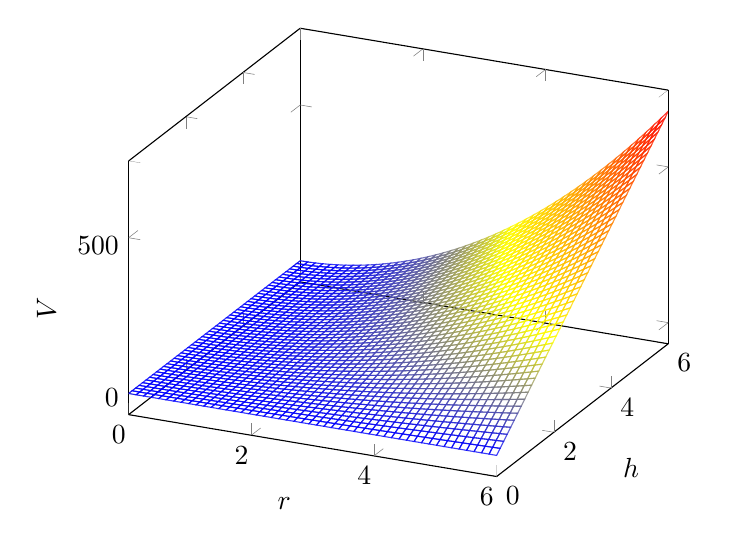
\begin{tikzpicture}
        \begin{axis}
        [xlabel={$r$}, ylabel={$h$}, zlabel={$V$}]
        \addplot3[
        surf,
        opacity=0.8,
        samples=50, samples y=50,
        domain=0:6, domain y=0:6, xlabel near ticks,
        mesh]
        {pi*x^2*y};
        \end{axis}
        \end{tikzpicture}
        %% picture now built in supplemental overleaf project to reduce compile time
    \fi
    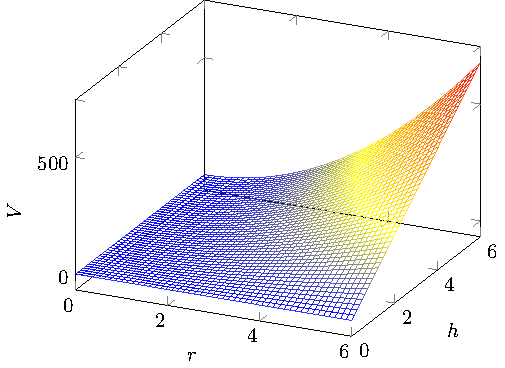
\includegraphics[width=.4\textwidth]{tikz-pictures/section-9.1-pic1-first-3d-graph-v1.pdf}\hfill
    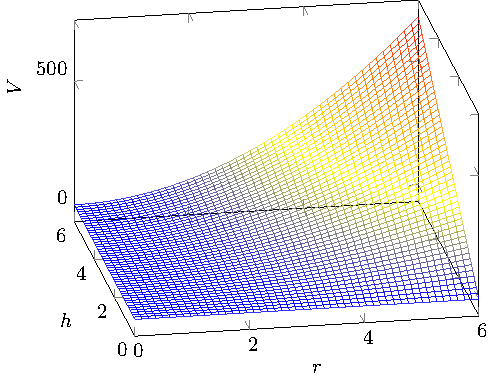
\includegraphics[width=.4\textwidth]{tikz-pictures/section-9.1-pic1-first-3d-graph-v2.pdf}\label{img:multivar-fn-graph}
\end{center}
You can produce a similar image at \url{https://wolframalpha.com} with the command 
\begin{center} 
    \href{https://www.wolframalpha.com/input/?i=plot+V%3Dpi*r%5E2*h+for+0%3C%3Dr%3C%3D6+and+0%3C%3Dh%3C%3D6}
    {\tt{plot V=pi*r\string^2*h for 0<=r<=6 and 0<=h<=6}}
\end{center}


\pagebreak 

Note that the domain of a function may depend on context (like the volume of a cylinder). If we are just given a mathematical function (with no context), then the domain consists of inputs for which the function is defined.

For our purposes, functions are most often undefined due to issues of:
\begin{itemize} 
    \item division by zero, 
    \item square root of a negative number, 
    \item logarithm of 0 or a negative number.
\end{itemize}

\begin{ex}
    Let $f(x,y)=4+5\sqrt{x^2+y}$. Sketch the domain of $f$.
\end{ex}

\vfill

\begin{ex}
    Let $g(x,y)=\dfrac{x+2y}{x^2-y^2}$. Sketch the domain of $g$.
\end{ex}

\vfill 

\pagebreak 

\subsection{Representing functions of two variables}
\begin{defn}[Graph of a function]
    The \emph{graph} of a function $f=f(x,y)$ is the set of points of the form $(x,y,f(x,y))$ where the point $(x,y)$ is in the domain of $f$.
\end{defn}
In other words, the graph of $f$ is the set of points $(x,y,z)$ where $z=f(x,y)$. The graph is called a \emph{surface}.

In any coordinate system, we need to make a choice about the directions of the axes. With three variables, we need three axes. This means 3D space!
\vspace{2in}

In order to represent 3D space visually, we use perspective drawing. We typically only draw the positive ends of each axis. In the drawing above, the $y$- and $z$-axes are essentially in the page, and the $x$-axis is coming out of the page at us.

Note how the axes are oriented with respect to each other! We use the ``right hand system.''%\footnote{Image below from \url{https://commons.wikimedia.org/wiki/File:Right_hand_rule_Cartesian_axes-permuted.svg}.} 

\begin{minipage}{.6\textwidth}
\begin{framed}
With your right hand, point your index finger in the direction of the positive $x$-axis and your middle finger in the direction of the positive $y$-axis. Your thumb will then point in the direction of the positive $z$-axis.
\end{framed}
\end{minipage}
\hfill \begin{minipage}{.3\textwidth}
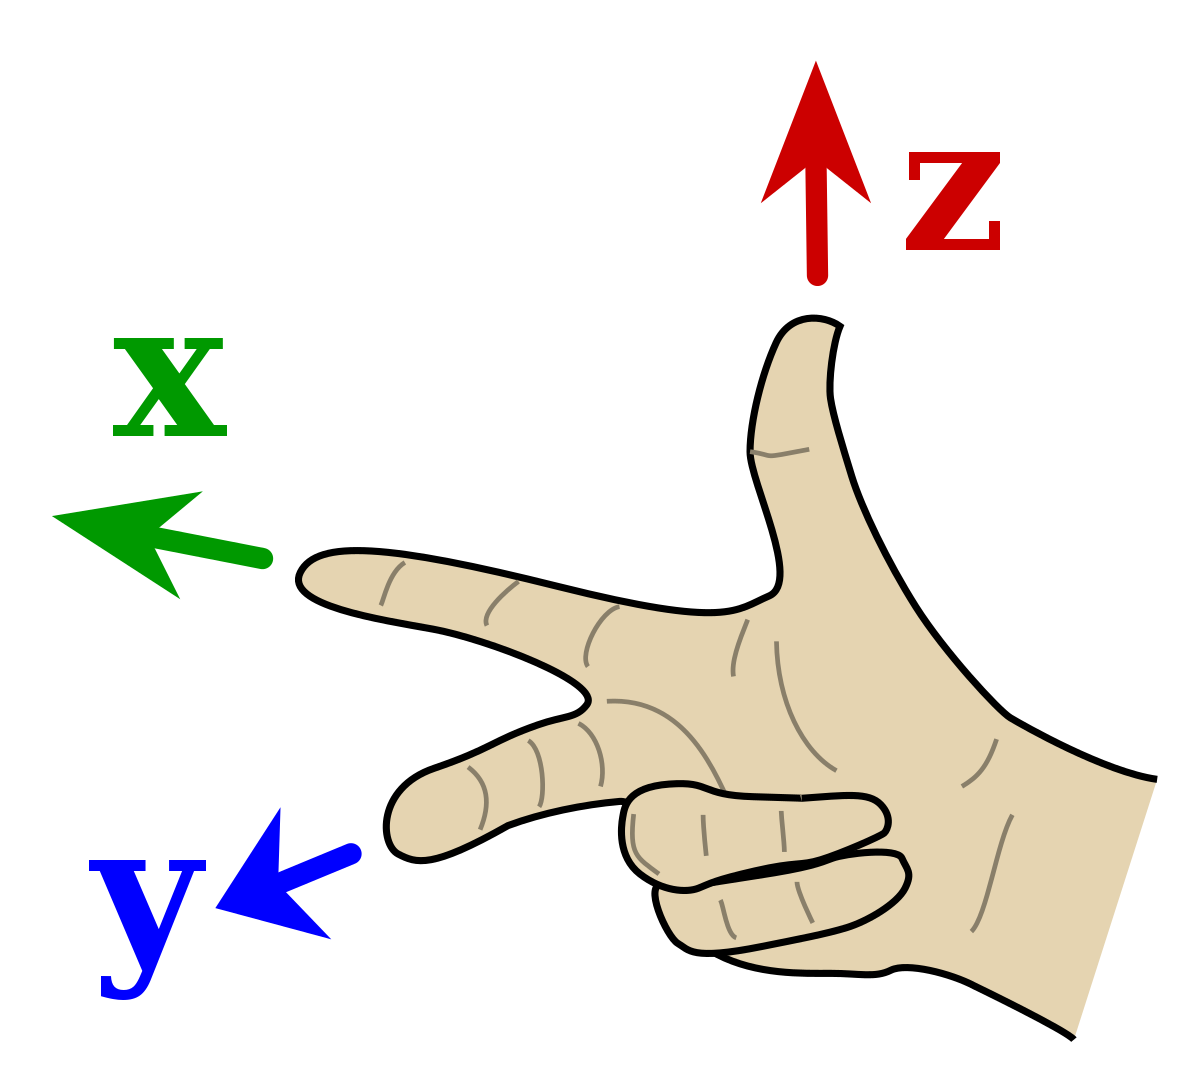
\includegraphics[width=\textwidth]{images/right hand rule axes.png}\label{img:right-hand-axes}
\end{minipage}

Some notation:
\begin{itemize}
    \item $\mathbb{R}$ is the set of real numbers, which we visualize with the real number line.
    \item $\mathbb{R}^2$ is the set of ordered pairs of real numbers $(x,y)$, which we visualize as the plane.
    \item $\mathbb{R}^3$ is the set of ordered triples of real numbers $(x,y,z)$, which we visualize as 3D space.
\end{itemize}

\vfill

In $\mathbb{R}^2$, there are four \emph{quadrants}: I, II, III, IV. In Quadrant I, $x,y\ge0$.
\medskip 

In $\mathbb{R}^3$, there are eight \emph{octants}. The \emph{first octant} is the region where $x,y,z\ge0$.
\bigskip 

Here's another way to think of the right hand system. If you are at the positive end of the $z$-axis and you look at the origin, you'll see the $x$- and $y$-axes oriented just as we normally orient them in 2D space.

\vspace{.5in}

\pagebreak 
Going further, if we have a function $f=f(x,y,z)$ of three variables, then its graph is the set of points $(x,y,z,f(x,y,z))$ where the point $(x,y,z)$ is in the domain of $f$. In other words, this is the set of points $(x,y,z,w)$ where $w=f(x,y,z)$. This graph is in $\mathbb{R}^4$ (i.e., in 4D!), which makes it pretty tricky to visualize. We can use similar ideas to think about $\mathbb{R}^n$ for any $n\ge1$.

\subsection{Some standard equations in three-space}
In $\mathbb{R}^3$, we have three coordinate planes: the $xy$-plane, the $xz$-plane, and the $yz$-plane. Each plane contains the axes in its name.
\begin{ex}
    Draw the three coordinate planes.
\end{ex}

\vspace{2in}

Note that when we graph a function $f(x,y)$, the domain of $f$ is part of (or all of) the $xy$-plane.

\begin{ex}
    Draw the (separate) graphs of the equations $y=0$, $z=2$, and $x=3$ in $\mathbb{R}^3$.
\end{ex}

\vspace{2.5in}

Recall: In $\mathbb{R}^2$, the distance between the points $P=(x_0,y_0)$ and $Q=(x_1,y_1)$ is 
\[
    \phantom{\sqrt{(x_1-x_0)^2+(y_1-y_0)^2}.}
\]

\vspace{1in}

\pagebreak 

In $\mathbb{R}^3$, we have a similar formula. 
\begin{framed}
    The distance between the points $P=(x_0,y_0,z_0)$ and $Q=(x_1,y_1,z_1)$ in $\mathbb{R}^3$ is
    \[
        \phantom{\sqrt{(x_1-x_0)^2+(y_1-y_0)^2+(z_1-z_0)^2}.}
    \]
\end{framed}

This comes from using the Pythagorean Theorem twice. See \href{https://activecalculus.org/vector/S-9-1-Functions.html#A-9-1-4}{Activity 9.1.5} in the textbook for details. (It's straightforward. In $\mathbb{R}^2$, we want the length of a diagonal of a rectangle. In $\mathbb{R}^3$, we want the length of a diagonal of a rectangular box.)

Any sphere can be described as the set of all points that are a fixed distance from a particular point. If we want a sphere of radius $r$ centered at $(x_0,y_0,z_0)$, then we want all points $(x,y,z)$ which are distance $r$ from $(x_0,y_0,z_0)$. In other words, we want
\[
    \phantom{\sqrt{(x-x_0)^2+(y-y_0)^2+(z-z_0)^2}=r.}
\]
We can square both sides to eliminate the square root and get the following:
\begin{framed}
    The equation of a sphere of radius $r$ centered at the point $(x_0,y_0,z_0)$ is
    \[
        \phantom{(x-x_0)^2+(y-y_0)^2+(z-z_0)^2=r^2.}
    \]
\end{framed}
\begin{ex}
    Write down the equation of a sphere of radius 3 centered at the point $(2,-4,0)$.
\end{ex}

\vspace{1in}

For the next problem, we will ``complete the square.'' The key idea is that 
\[
    x^2+ax=\left(x+\dfrac{a}{2}\right)^2-\left(\dfrac{a}{2}\right)^2.\]
    \emph{(For a refresher on completing the square, check out \href{https://tutorial.math.lamar.edu/classes/alg/SolveQuadraticEqnsII.aspx}{Paul's Notes}.)}
\begin{ex}
    The equation $x^2+y^2+z^2+6x-2y+10z=14$ defines a sphere. Where is it centered and what is its radius?
\end{ex}
\vfill


\newlecture

\setcounter{section}{1}
%\def\textbookchapter{Chapter 9: Multivariable and Vector Functions}
\def\coursetopicnumber{I}
\def\textbooksection{9.2} % corresponding textbook section
\def\topic{Vectors} % this is the printed title
\def\shorttopic{Vectors} % short topic
\def\textbookname{Active Calculus} % this is the textbook
\def\textbooksectionurl{https://activecalculus.org/vector/S-9-2-Vectors.html} % URL for textbook section
\def\handoutday{} % this is the printed date

%%%%%%%%% DOCUMENT CONTENT STARTS BELOW

\thispagestyle{plain}
\topstuff
\section{\topic{} \booklink{}}
%\section{\href{\textbooksectionurl}{\topic{}}}
\subsection{Representations of vectors}
\begin{defn}[Vector]
A \emph{vector} (or \emph{displacement vector}) is an arrow that has a tail at one end and a head at the other end.
\end{defn}
\vspace{1in}

Vectors exist in $\mathbb{R}$, $\mathbb{R}^2$, $\mathbb{R}^3$, etc. We'll focus on vectors in $\mathbb{R}^2$ since any drawing surface is essentially $\mathbb{R}^2$. Note that the ideas we'll see apply in any dimension.

Any vector has two important characteristics: 
\begin{itemize}
    \item its \emph{direction} (i.e., \hide{the direction in which it points), and}
    \item its \emph{magnitude} (i.e., \hide{its length).}
\end{itemize}

\begin{framed}
    Two vectors are equal if \hide{they point in the same direction and have the same magnitude.} \\ \mbox{} \\ \mbox{} 
\end{framed}

\vfill

To distinguish vectors from real numbers, we put an arrow over the vector's name (like $\vec{v}$) to indicate that it is a vector.  In most books -- including ours! --  vectors are written in bold (like $\mathbf{v}$).


Any vector $\vec{v}$ can be thought of as an arrow from a point $P$ to a point $Q$. We write $\vec{v}=\vec{PQ}$.

%% The following command gives empty axes.
\newcommand{\AxesForVectors}{
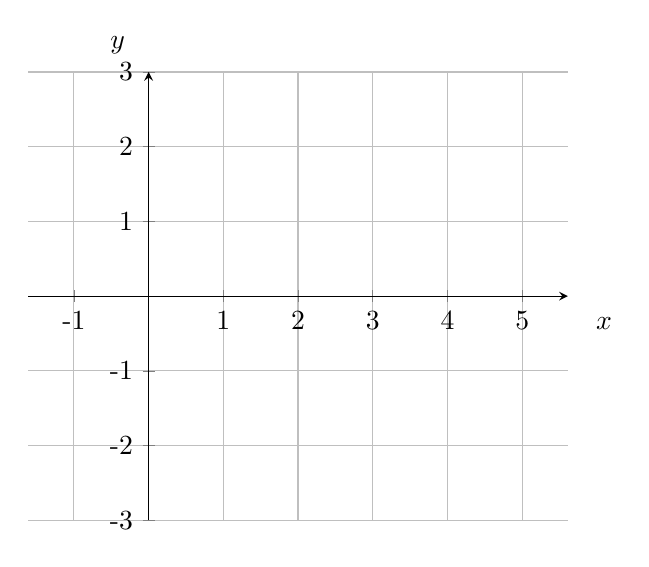
\begin{tikzpicture}
  \begin{axis}[grid=both,ymin=-3,ymax=3,xmax=5,xmin=-1,xtick={-1,0,1,2,3,4,5},ytick={-3,-2,-1,0,1,2,3},xticklabels={-1,0,1,2,3,4,5},yticklabels={-3,-2,-1,0,1,2,3},
               axis lines = middle,axis equal=true,xlabel=$x$,ylabel=$y$,label style =
               {at={(ticklabel cs:1.1)}}]
  \end{axis}
\end{tikzpicture}}

\begin{ex}
    Let $P=(1,2)$ and $Q=(4,0)$. Draw $\vec{v}=\vec{PQ}$. If we shift $\vec{v}$ to start at the point $(0,1)$, where does it end? What if we shifted $\vec{v}$ to start at the origin?
    
    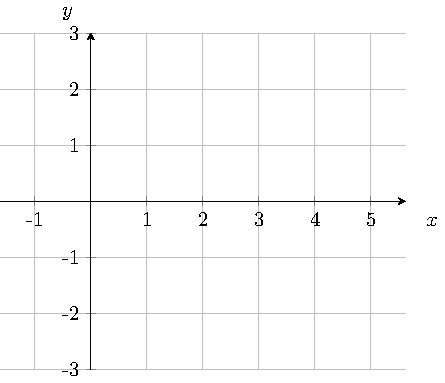
\includegraphics[width=.3\textwidth]{tikz-pictures/section-9.2-pic1-axes-for-vectors.pdf}
\end{ex}

\pagebreak 

Let $O$ denote the origin. Just as in the previous example, any vector can be moved so that it starts at $O$.

\begin{defn}[Standard position, component form, position vector]
\label{defn:position-vector}
    When a vector starts at the origin, we say that it is in \emph{standard position}.
    
    If a vector $\vec{v}$ in standard position ends at a point $P=(a,b)$, we write 
    \[
        \vec{v}=\vec{OP}=\phantom{\langle a,b\rangle,}\hspace{2in}
    \]
    which is the \emph{component form of $\vec{v}$}. This is a \emph{position vector} for the point $P$.
\end{defn}

\vspace{1in}

\begin{ex}
    For $P=(2,-1)$ and $Q=(4,2)$, let $\vec{v}=\vec{PQ}$. Draw $\vec{v}$, then draw $\vec{v}$ as a position vector, and then write $\vec{v}$ in component form.
    
    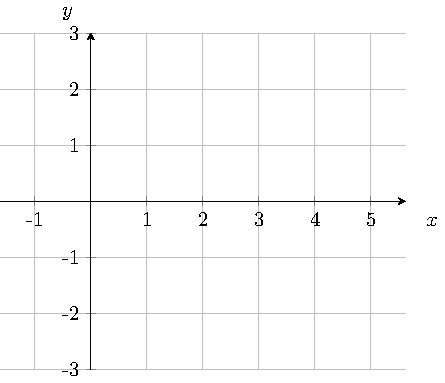
\includegraphics[width=.3\textwidth]{tikz-pictures/section-9.2-pic1-axes-for-vectors.pdf}
\end{ex}

\begin{framed}
    In general, if $\vec{v}=\vec{PQ}$ with $P=(x_1,y_1)$ and $Q=(x_2,y_2)$, then 
    \medskip 

    $\vec{v}=\phantom{\langle x_2-x_1, y_2-y_1\rangle.}$\\ \mbox{}
\end{framed}
\begin{ex}
    For $P=(4,-1)$ and $Q=(-2,3)$, let $\vec{v}=\vec{PQ}$. Write $\vec{v}$ in component form.
\end{ex}

\vfill

\subsection{Equality of vectors}
\begin{framed} 
    Two position vectors $\vec{u}=\langle u_1,u_2\rangle$ and $\vec{v}=\langle v_1,v_2\rangle$ are equal if and only if \hide{$u_1=v_1$ and $u_2=v_2$.}\\
\end{framed}
Note: These boxed statements extend to vectors in $\mathbb{R}^3$ (and beyond).
\pagebreak 

\subsection{Operations on vectors}
\begin{defn}[Vector addition]
    For vectors $\vec{v}=\langle v_1,v_2\rangle$ and $\vec{w}=\langle w_1,w_2\rangle$ in $\mathbb{R}^2$, we add $\vec{v}$ and $\vec{w}$ as follows:
    \[
        \vec{v}+\vec{w}=\langle v_1,v_2\rangle+\langle w_1,w_2\rangle = \phantom{\langle v_1+w_1,v_2+w_2\rangle.}\hspace{2in}
    \]
\end{defn}
We call this \emph{component-wise addition}. Vector addition in $\mathbb{R}^3$ works the same way.

\begin{ex}
    Let $\vec{v}=\langle 2,-3\rangle$ and $\vec{w}=\langle 5,2\rangle$. Compute $\vec{v}+\vec{w}$.
\end{ex}

\vspace{1in}

\begin{defn}[Scalar]
    A \emph{scalar} is a real number.
\end{defn}
\begin{ex}
    Write down a few examples of scalars.
\end{ex}
%Here are a few examples of scalars: $3/5$, $-\pi$, $142.7$, and $0$.

\vspace{1in}

We can multiply any vector by a scalar.
\begin{defn}[Scalar multiple]
    If $c$ is a scalar and $\vec{v}$ is a vector, then $c\vec{v}$ is a vector. We call $c\vec{v}$ a \emph{scalar multiple} of $\vec{v}$.
\end{defn}

In component form, if $\vec{v}=\langle v_1,v_2\rangle$, then $c\vec{v}=c\langle v_1,v_2\rangle=\phantom{\langle c v_1, cv_2\rangle.}$

\begin{ex}\label{ex:parallel-vectors}
    For $\vec{v}=\langle 2,1\rangle$, compute $c\vec{v}$ for $c=3$, $c=-1$, and $c=0$. Then draw $\vec{v}$ and these vectors on the axes below.
\end{ex}
\mbox{} \hfill 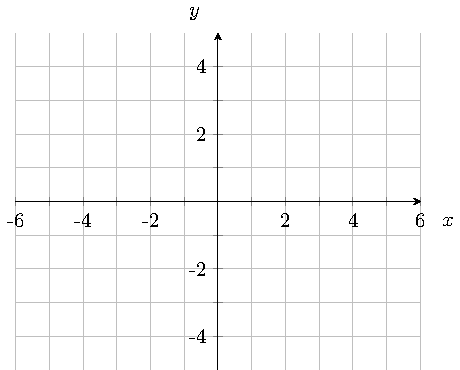
\includegraphics[width=.4\textwidth]{tikz-pictures/section-9.2-pic2-axes-for-more-vectors.pdf}

\vfill

\noindent Notation: For any vector $\vec{v}$, $-\vec{v}$ means $(-1)\vec{v}$.
\begin{defn}[Zero vector]
    The \emph{zero vector}, written $\vec{0}$, is the vector whose components are all 0. In $\mathbb{R}^2$, $\vec{0}=\langle 0,0\rangle$. In $\mathbb{R}^3$, $\vec{0}=\langle 0,0,0\rangle$.
\end{defn}

\pagebreak 

Visually, we see that the vectors in Exercise~\ref{ex:parallel-vectors} are parallel to each other. Here's our definition.

\begin{defn}[Parallel vectors]
    Vectors $\vec{u}$ and $\vec{v}$ are \emph{parallel} if \hide{one of them is a scalar multiple of the other.}
\end{defn}

\vspace{.7in}

\begin{ex}
    Consider the vectors $\vec{v}=\langle 1,2\rangle$, $\vec{w}=\langle 3,-4\rangle$, and $\vec{u}=\langle -5,-10\rangle$. Are any of these vectors parallel to each other?
\end{ex}

\vspace{1.5in}

Now that we can add vectors and multiply vectors by scalars, we can subtract vectors.
\begin{defn}[Vector subtraction]
    For vectors $\vec{v}$ and $\vec{w}$, we subtract $\vec{w}$ from $\vec{v}$ as follows:
    \[
        \vec{v}-\vec{w}=\phantom{\vec{v}+(-1)\vec{w}.}\hspace{2in}
    \]
    In particular, if $\vec{v}=\langle v_1,v_2\rangle$ and $\vec{w}=\langle w_1,w_2\rangle$ are vectors in $\mathbb{R}^2$, then
    \[
        \vec{v}-\vec{w}=\langle v_1,v_2\rangle-\langle w_1,w_2\rangle = \phantom{\langle v_1-w_1,v_2-w_2\rangle.}\hspace{2in}
    \]
\end{defn}
%(In other words, $-\vec{w}$ means $(-1)\vec{w}$.)
\bigskip 

\begin{defn}[Standard unit vectors]
    In $\mathbb{R}^2$, we have two special vectors: 
    \[
        \ii =\langle 1,0\rangle \text{ and } \jj =\langle 0,1\rangle.
    \]
    In $\mathbb{R}^3$, we have three special vectors:
    \[
        \ii =\langle 1,0,0\rangle \text{ and } \jj =\langle 0,1,0\rangle \text{ and } \kk =\langle 0,0,1\rangle.
    \]
    These are all \emph{standard unit vectors}.
\end{defn}

\begin{ex}
    Draw $\ii $ and $\jj $ in $\mathbb{R}^2$. Draw $\ii $, $\jj $, and $\kk $ in $\mathbb{R}^3$.
\end{ex}

\vspace{1.5in}

\begin{ex}
    Let $\vec{v}=3\ii +4\jj +6\kk $. Write $\vec{v}$ in component form.
\end{ex}

\vspace{1in}

\pagebreak 
In terms of the standard unit vectors, 
\begin{multicols}{2}
    \begin{itemize}
        \item $\langle a,b\rangle = \phantom{a\ii +b\jj }$
        \item $\langle a,b,c\rangle = \phantom{a\ii +b\jj +c\kk .}$
    \end{itemize}
\end{multicols}
\bigskip 

We have two equivalent notations for vectors: component form with the angle brackets; and in terms of standard unit vectors. Both notations are useful.

\subsection{Properties of vector operations}
We now know how to add vectors together and how to multiply them by scalars. In general, a set of vectors like this forms a \emph{vector space}. (For a course on vector spaces, take Linear Algebra!)

In a vector space, the following properties which hold for any vectors $\vec{u}, \vec{v}, \vec{w}$ and any scalars $a$ and $c$:
\begin{enumerate}[label=\arabic*.]
    \item $\vec{u}+\vec{v}=\phantom{\vec{v}+\vec{u}}$ \hfill (Commutative property of addition)
    \item $(\vec{u}+\vec{v})+\vec{w}=\phantom{\vec{u}+(\vec{v}+\vec{w})}$ \hfill (Associative property of addition)
    \item $\vec{v}+\vec{0}=\phantom{\vec{v}}$ \hfill (Additive identity)
    \item $\vec{v}+(-\vec{v})=\phantom{\vec{0}}$ \hfill (Additive inverse)
    \item $c(\vec{u}+\vec{v})=\phantom{c\vec{u}+c\vec{v}}$ \hfill (Distributive property 1)
    \item $(a+c)\vec{v}=\phantom{a\vec{v}+c\vec{v}}$ \hfill (Distributive property 2)
    \item $0\vec{v}=\phantom{\vec{0}}$ \hfill (Multiplication by zero scalar)
    \item $c\vec{0}=\phantom{\vec{0}}$ \hfill (Multiplication of zero vector)
    \item $1\vec{v}=\phantom{\vec{v}}$ \hfill (Multiplicative identity)
    \item $a(c\vec{v})=\phantom{(ac)\vec{v}}$ \hfill (Associative property of scalar multiplication)
\end{enumerate}
Each property is relatively straightforward to show if you write each vector in component form.
\bigskip 

\begin{ex}
    Let $\vec{v}=2\ii -3\jj $ and $\vec{w}=5\ii +2\jj $.
    Suppose 
    \[
        2\vec{v}+3\vec{x}=\vec{w}+\jj .
    \]
    Solve for $\vec{x}$.
\end{ex}

\pagebreak 

\subsection{Geometric interpretation of vector operations}
We know how to visualize scalar multiplication. There are nice geometric interpretations for vector addition and subtraction, too.

For vector addition, we use the ``head-to-tail'' method. If we want to compute $\vec{v}+\vec{w}$, we select a starting point $P$, draw $\vec{v}$ as starting at $P$ and ending at some point $Q$, and then draw $\vec{w}$ as starting at $Q$ and ending at some point $R$. 

\vspace{2in}

In other words, if $\vec{v}=\vec{PQ}$ and $\vec{w}=\vec{QR}$, then $\vec{v}+\vec{w}=\vec{PR}$. This means that $\vec{v}$, $\vec{w}$, and $\vec{v}+\vec{w}$ form three sides of a triangle.

For the picture above, we connected the head of $\vec{v}$ to the tail of $\vec{w}$. Since $\vec{v}+\vec{w}=\vec{w}+\vec{v}$, we could draw the vectors in the opposite order. This gives rise to the ``parallelogram rule'' for adding vectors.

\vspace{2in}

For vector subtraction, we have two approaches. First, to compute $\vec{v}-\vec{w}$, we know that
\[
    \vec{v}-\vec{w}=\vec{v}+(-\vec{w}).
\]
So, if we can draw $\vec{v}$ and $-\vec{w}$, then we can add them with the method above.

Alternatively, we can draw the vectors $\vec{v}$ and $\vec{w}$ both starting from the same point. Then, draw the vector from the head of $\vec{w}$ to the head of $\vec{v}$. That vector is $\vec{v}-\vec{w}$.

\vspace{2in}

\pagebreak 

\subsection{The magnitude of a vector}
\begin{defn}[Magnitude]
    The \emph{magnitude} of a vector $\vec{v}$, denoted $|\vec{v}|$, is the length of $\vec{v}$. (Note: Some other books write this as $||\vec{v}||$.)
\end{defn}

\begin{ex}
    Draw the vector $\vec{v}=\langle 3,-4\rangle$. Compute $|\vec{v}|$.
\end{ex}

\vspace{1.5in}

\begin{framed}
    In general, if $\vec{v}=\langle v_1,v_2\rangle$ is a vector in $\mathbb{R}^2$, then $|\vec{v}|$ is the distance from the origin $(0,0)$ to the point $(v_1,v_2)$. Thus,
    \[
        |\vec{v}|=\phantom{\sqrt{v_1^2+v_2^2}.}\hspace{2in}
    \]
\end{framed}

\begin{framed} 
    More generally, if $\vec{v}=\langle v_1,v_2,\dots,v_n\rangle$ is a vector in $\mathbb{R}^n$, then 
    \[
        |\vec{v}|=\phantom{\sqrt{v_1^2+v_2^2+\dots+v_n^2}.}\hspace{2in}
    \]
\end{framed}

Two notes:
\begin{multicols}{2}
\begin{itemize}
    \item For any scalar $c$, $|c\vec{v}|=|c|\,|\vec{v}|$.
    \item In general, $|\vec{v}+\vec{w}|\ne |\vec{v}|+|\vec{w}|$.
\end{itemize}
\end{multicols}
\bigskip 

\begin{defn}[Unit vector]
    A \emph{unit vector} is a vector $\vec{v}$ with $|\vec{v}|=1$.
\end{defn}
Unit vectors have magnitude 1. Some examples are $\ii$, $\jj$, and $\kk$. And there are many more.

\begin{ex}
    Which of the following are unit vectors?
    \begin{enumerate}
        \item $\vec{v}=\left\langle 1/2,\sqrt{3}/2\right\rangle$
        \item $\vec{w}=\left\langle1,-1,1\right\rangle$
        \item $\vec{u}=\left\langle1/2,1/2,1/2,1/2\right\rangle$
    \end{enumerate}
\end{ex}
\pagebreak 

\begin{ex}
If $\vec{v}$ is any vector other than the zero vector, let $c=1/|\vec{v}|$ and compute $|c\vec{v}|$.
\end{ex}

\vspace{.8in}

\begin{framed}
    \noindent When $\vec{v}\ne \vec{0}$, we can easily find a unit vector $\vec{u}$ that points in the same direction of $\vec{v}$: 
    \[
        \hspace{-3in}\vec{u}=\phantom{\frac{1}{|\vec{v}|}\vec{v}.}
    \]
\end{framed}

\noindent Lingo: When we scale a vector $\vec{v}$ to get a unit vector $\vec{u}$, we have \emph{normalized} $\vec{v}$.

\vfill 

\begin{ex}
    Let $\vec{v}=5\ii -12\jj $.
    \begin{enumerate}
        \item Find a unit vector $\vec{u}$ in the direction of $\vec{v}$.
        \vspace{1.3in}
        \item Find a vector $\vec{w}$ of length 4 in the direction opposite from $\vec{v}$. Write $\vec{w}$ in terms of the standard unit vectors.
        \vspace{1.3in}
    \end{enumerate}
\end{ex}

A \emph{unit circle} is a circle of radius 1. When centered at $(0,0)$, its equation is $x^2+y^2=1$. Starting from the point $(1,0)$, if you travel CCW a distance $\theta$, you get to the point $P=(\cos\theta,\sin\theta)$.

Note that $\theta$ is the angle (in radians) measured above the positive $x$-axis.

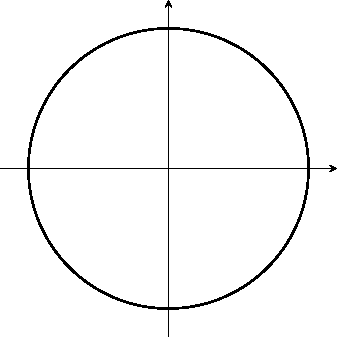
\includegraphics[width=.35\textwidth]{tikz-pictures/section-9.2-pic3-unit-circle.pdf}

\pagebreak 

Here's a useful observation. If $\vec{u}$ is a unit vector in standard position in $\mathbb{R}^2$ (meaning its tail is at the origin), then the head of $\vec{u}$ is on the unit circle. Since every point on the unit circle is of the form $(\cos\theta,\sin\theta)$ for some real number $\theta$, every unit vector $\vec{u}$ in $\mathbb{R}^2$ is of the form
\[
    \vec{u}=\phantom{\langle \cos\theta,\sin\theta\rangle}
\]
for some real number $\theta$.

More generally, if $\vec{v}$ is a vector in $\mathbb{R}^2$ that starts at the origin and has magnitude $r$ for some positive number $r$, then the head of $\vec{v}$ is on the circle of radius $r$ centered at the origin.

\begin{ex}
    Let $r>0$ be a scalar. Let $\vec{v}$ be the vector of length $r$ from the origin at an angle $\theta$ above the positive $x$-axis. Write $\vec{v}$ in terms of the standard unit vectors.
\end{ex}

\vspace{3in}

\begin{ex}
    Find a vector $\vec{v}$ of length 5 that points at an angle of $60^\circ$ above the positive $x$-axis.
\end{ex}

\vfill

\newlecture

\setcounter{section}{2}
%\def\textbookchapter{Chapter 9: Multivariable and Vector Functions}
\def\coursetopicnumber{I}
\def\textbooksection{9.3} % corresponding textbook section
\def\topic{The Dot Product} % this is the printed title
\def\shorttopic{Dot product} % short topic
\def\textbookname{Active Calculus} % this is the textbook
\def\textbooksectionurl{https://activecalculus.org/vector/S-9-3-Dot-Product.html} % URL for textbook section
\def\handoutday{} % this is the printed date

%%%%%%%%% DOCUMENT CONTENT STARTS BELOW

\thispagestyle{plain}
\topstuff
\section{\topic{} \booklink{}}
\label{sec:dot-product}
The dot product gives us a way to ``multiply'' one vector by another vector. We start with a computational definition, and we will see that it gives us some really useful information about the angle between the vectors.

\subsection{Dot product}
\begin{defn}[Dot product in $\mathbb{R}^2$]
    Suppose $\vec{u}=\langle u_1,u_2\rangle$ and $\vec{v}=\langle v_1,v_2\rangle$ are vectors in $\mathbb{R}^2$.
    
    The \emph{dot product} of $\vec{u}$ and $\vec{v}$ is 
    \[
        \vec{u}\dotp \vec{v}=\langle u_1,u_2\rangle \dotp \langle v_1,v_2\rangle = \hspace{2in}
    \]
\end{defn}

\begin{defn}[Dot product in $\mathbb{R}^3$]
    Suppose $\vec{u}=\langle u_1,u_2,u_3\rangle$ and $\vec{v}=\langle v_1,v_2,v_3\rangle$ are vectors in $\mathbb{R}^3$.
    \bigskip
    
    The \emph{dot product} of $\vec{u}$ and $\vec{v}$ is 
    \[
        \vec{u}\dotp \vec{v}=\langle u_1,u_2,u_3\rangle \dotp \langle v_1,v_2,v_3\rangle = \hspace{2in}
    \]

\end{defn}

\noindent Note: Some people call the dot product an \emph{internal product} or a \emph{scalar product}.

\bigskip
We have the same definition of the dot product for vectors in $\mathbb{R}^n$ for any $n$:

\vspace{1in}

\begin{ex}
Compute $\vec{u}\dotp\vec{v}$ for the following pairs of vectors.
	\begin{multicols}{2}
    \begin{enumerate}
        \item $\vec{u}=\langle 2,3,4\rangle$ and $\vec{v}=\langle -1,-5,0\rangle$.
        \item $\vec{u}=6\ii -4\jj $ and $\vec{v}=-5\jj $.
    \end{enumerate}
    \end{multicols}
\end{ex}

\vfill

\pagebreak 

\begin{ex}
    Say $\vec{v}=\langle v_1,v_2,v_3\rangle$.
	\begin{multicols}{3}
    \begin{enumerate}
        \item What is $\vec{v}\dotp\vec{v}$?
        \item What is $\vec{0}\dotp\vec{v}$?
        \item What is $\ii \dotp\jj $?
    \end{enumerate}
    \end{multicols}
\end{ex}

\vspace{1.3in}

Here are some properties that the dot product satisfies.
\begin{thm}\label{thm:dot-product-properties}
    Say $\vec{u}, \vec{v}, \vec{w}$ are vectors in $\mathbb{R}^n$ for any $n$, and say $c$ is any scalar. Then
    \begin{enumerate}
        \item $\vec{u}\dotp\vec{v}=\phantom{\vec{v}\dotp\vec{u}}$ \hfill (Commutative property)
        \item $c\,(\vec{u}\dotp\vec{v})=\phantom{(c\,\vec{u})\dotp\vec{v}=\vec{u}\dotp(c\,\vec{v})}$ \hfill (Associative property)
        \item $\vec{u}\dotp (\vec{v}+\vec{w})=\phantom{(\vec{u}\dotp\vec{v})+(\vec{u}\dotp\vec{w})}$ \hfill (Distributive property)
        \item $\vec{v}\dotp\vec{v}=$ \hfill (Dot product relation to magnitude)
    \end{enumerate}
\end{thm}
\noindent (These are straightforward to prove if you write $\vec{u}$, $\vec{v}$, and $\vec{w}$ in terms of their components.)

\subsection{Angle between two vectors}
The dot product of two vectors gives us some useful information about the angle between the vectors. To see this, we need the Law of Cosines.

\vspace{2in}

\begin{ex}
    For vectors $\vec{u}$ and $\vec{v}$, draw $\vec{u}$ and $\vec{v}$ as coming out of the same point. Connect their heads with the vector $\vec{u}-\vec{v}$. What does the Law of Cosines say about the resulting triangle?
\end{ex}

\pagebreak 

\begin{ex}
    In the previous exercise, we found $|\vec{u}-\vec{v}|^2=|\vec{u}|^2+|\vec{v}|^2-2|\vec{u}||\vec{v}|\cos\theta$. Use properties from Theorem~\ref{thm:dot-product-properties} to solve for $\vec{u}\dotp\vec{v}$.
\end{ex}

\vspace{2.5in}

\begin{framed}
    \begin{thm}\label{thm:dot-prod-thm}
        For vectors $\vec{u}$ and $\vec{v}$ in $\mathbb{R}^n$ with $\theta$ the angle between $\vec{u}$ and $\vec{v}$, 
        \[
            \hspace{-2in}\vec{u}\dotp\vec{v}=\phantom{|\vec{u}|\,|\vec{v}|\cos(\theta),}
        \]
    \end{thm}
\end{framed}
Note that we can always take $\theta$ to be between 0 and $\pi$ (i.e., between 0 and 180 degrees).

\subsection{Dot product and orthogonality}
For any nonzero vectors $\vec{u}$ and $\vec{v}$, since $|\vec{u}|>0$ and $|\vec{v}|>0$, $\vec{u}\dotp\vec{v}$ has the same sign as $\cos(\theta)$.

\noindent Recall: $\cos(\theta)$ is positive when $0\le\theta<\pi/2$, zero when $\theta=\pi/2$, and negative when $\pi/2<\theta\le\pi$.\\
\bigskip

\noindent \begin{minipage}{.6\textwidth}
\begin{itemize}
    \item If $\vec{u}\dotp\vec{v}>0$, then $\cos(\theta)>0$, and the angle between $\vec{u}$ and $\vec{v}$ is \\ \\ \\
    \item If $\vec{u}\dotp\vec{v}<0$, then $\cos(\theta)<0$, and the angle between $\vec{u}$ and $\vec{v}$ is \\ \\ \\
    \item If $\vec{u}\dotp\vec{v}=0$, then $\cos(\theta)=0$, and the angle between $\vec{u}$ and $\vec{v}$ is \\
\end{itemize}
\end{minipage}

\pagebreak
\begin{defn}[Orthogonal]
    If $\vec{u}\dotp\vec{v}=0$, then we say $\vec{u}$ and $\vec{v}$ are \emph{orthogonal}.
\end{defn}
\bigskip

\begin{defn}[Perpendicular]
    If the angle between two nonzero vectors is a right angle, then we say the vectors are \emph{perpendicular} to each other, denoted $\vec{u}\perp\vec{v}$.
\end{defn}
Thus, for nonzero vectors, ``orthogonal'' and ``perpendicular'' mean the same thing. \medskip 


\begin{framed}
    The dot product gives us an easy way to determine whether two nonzero vectors are perpendicular to each other or not -- we just check to see if their dot product is zero or not!
\end{framed}
\bigskip 

\begin{ex}
    Let $\vec{v}=\langle 2,4,-1\rangle$ and $\vec{w}=\langle 3,0,8\rangle$. Are $\vec{v}$ and $\vec{w}$ perpendicular to each other? If not, at what kind of angle do they meet?
\end{ex}
\vfill

\begin{ex}
    Say $\vec{u}$ is a vector of length 3, $\vec{v}$ is a vector of length 4, and the angle between them is $\theta=\pi/3$. Compute $\vec{u}\dotp\vec{v}$.
\end{ex}

\vfill

\pagebreak 

Also, since $\vec{u}\dotp\vec{v}=|\vec{u}| |\vec{v}|\cos(\theta)$, we can solve for $\theta$ to compute the angle between two vectors in $\mathbb{R}^n$ for any $n$. Even if we can't visualize it, there's a way to think about that angle.
\[
    \hspace{-3in}\cos(\theta)=\phantom{\dfrac{\vec{u}\dotp\vec{v}}{|\vec{u}||\vec{v}|}.}
\]
\bigskip

\begin{ex}
    Let $\vec{u}=\langle \sqrt{3},1,0\rangle$, $\vec{v}=\langle 1,\sqrt{3},0 \rangle$, $\vec{w}=\langle 1,\sqrt{3},2\sqrt{3}\rangle$.
	\begin{enumerate}
    	\item Compute $\vec{u}\dotp\vec{v}$.\vspace{.8in}
    	\item What is the angle between $\vec{u}$ and $\vec{v}$?\vfill
        \item What is the angle between $\vec{u}$ and $\vec{w}$?\\ \\ \vfill
	\end{enumerate}
\end{ex}

\pagebreak

\subsection{Work, force, and displacement}
Recall that the work $W$ done by a constant force $F$ in moving an object a distance $d$ is $W=Fd$. This rule works if the force acts in the direction of motion. For units, if $F$ is in newtons ($N$) and distance is in meters ($m$), then work is in joules ($J$), where $1\,J=1\,N\cdot m$. (Or force is in pounds, distance is in feet, and work is in foot-pounds.)

If the force is not in the direction of motion (perhaps at an angle), then we need to first compute the amount of force that is in the direction of motion before we multiply it by $d$ to compute work.

\vspace{3in}

Vectors can greatly simplify our calculations. We can represent the force and distance traveled by vectors $\vec{F}$ and $\vec{d}$. By Theorem \ref{thm:dot-prod-thm}, 
\[
    \vec{F}\dotp\vec{d}=\phantom{|\vec{F}| |\vec{d}| \cos(\theta),}
\] 
so $W=\phantom{\vec{F}\dotp\vec{d}.}$\\

\begin{ex}
    A force $\vec{F}=\langle 3,3,2\rangle$ (in newtons) is applied to move an object along a line segment from $P=(1,1,0)$ to $Q=(6,6,0)$ (in meters). What is the work done in moving the object?
\end{ex}

\pagebreak 

\subsection{Projections}
In many applications, it is useful to decompose a vector into a sum of two vectors that have nice properties.
\begin{defn}[Projection of $\vec{u}$ onto $\vec{v}$]
    Let $\vec{u}$ and $\vec{v}$ be vectors with $\vec{v}\ne\vec{0}$. The \emph{orthogonal projection of $\vec{u}$ onto $\vec{v}$}, denoted $\proj_{\vec{v}}\,(\vec{u})$ is the vector formed by the ``shadow'' cast by $\vec{u}$ onto the line through $\vec{v}$.
\end{defn}

\vspace{2in}

\noindent The key is that the line dropping down from $\vec{u}$ forms a right angle with the line through $\vec{v}$.
\begin{thm}[Calculation of the orthogonal projection of $\vec{u}$ onto $\vec{v}$]
    For vectors $\vec{u}$ and $\vec{v}$ with $\vec{v}\ne\vec{0}$, 
    \[
        \hspace{-3in}\proj_{\vec{v}}\,(\vec{u})=
    \phantom{\left(\frac{\vec{u}\dotp\vec{v}}{\vec{v}\dotp\vec{v}}\right)\vec{v}.}
    \]
\end{thm}
\bigskip 

\begin{defn}[Component of $\vec{u}$ in the direction of $\vec{v}$]
    The \emph{component of $\vec{u}$ in the direction of $\vec{v}$}, denoted $\comp_{\vec{v}}(\vec{u})$, is the magnitude of $\proj_{\vec{v}}(\vec{u})$.
\end{defn}
Since 
$\proj_{\vec{v}}({\vec{u}})
=\dfrac{\vec{u}\dotp\vec{v}}{\vec{v}\dotp\vec{v}}\vec{v}
=\dfrac{\vec{u}\dotp\vec{v}}{|\vec{v}|^2}\vec{v}
=\left(\dfrac{\vec{u}\dotp\vec{v}}{|\vec{v}|}\right)\left(\dfrac{1}{|\vec{v}|}\vec{v}\right)$, and since $\dfrac{1}{|\vec{v}|}\vec{v}$ is a unit vector,
\[
    \comp_{\vec{v}}(\vec{u}) = \phantom{\dfrac{\vec{u}\dotp\vec{v}}{|\vec{v}|}}\hspace{2in}
\]

\begin{ex}
    For $\vec{u}=\langle 4,1\rangle$ and $\vec{v}=\langle 3,4\rangle$, draw $\vec{u}$, $\vec{v}$, and the projection of $\vec{u}$ onto $\vec{v}$. 
    
    Then compute the projection of $\vec{u}$ onto $\vec{v}$ and the component of $\vec{u}$ in the direction of $\vec{v}$.
\end{ex}

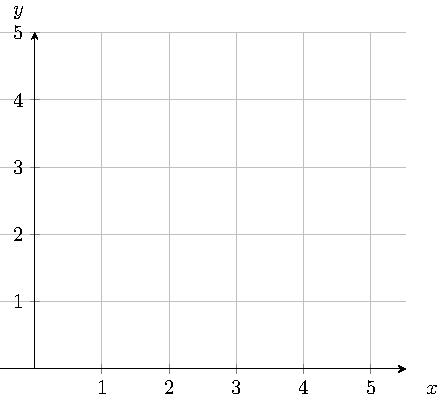
\includegraphics[scale=.8]{tikz-pictures/section-9.2-pic4-axes-for-projection-example.pdf}

\pagebreak 
\begin{ex}
    Still with $\vec{u}=\langle 4,1\rangle$ and $\vec{v}=\langle 3,4\rangle$, write $\vec{u}$ as a sum of vectors: one which is parallel to $\vec{v}$ and one which is perpendicular to $\vec{v}$.
\end{ex}
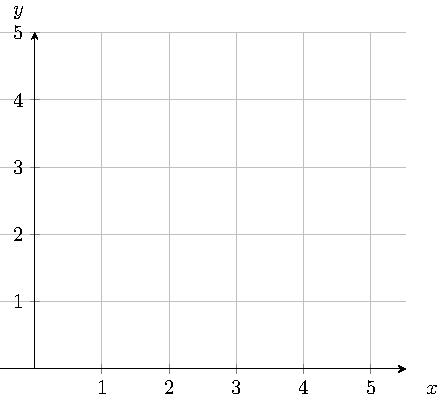
\includegraphics[scale=.8]{tikz-pictures/section-9.2-pic4-axes-for-projection-example.pdf}

The idea that we used in the above exercise works in general.\\
\begin{thm}[Orthogonal decomposition]
    For vectors $\vec{u}$ and $\vec{v}$ with $\vec{v}\ne\vec{0}$, we can write $\vec{u}$ as a sum of two vectors
    \[\vec{u}=\proj_{\vec{v}}(\vec{u})+\proj_{\perp\vec{v}}(\vec{u})\] where
    \begin{multicols}{2}
    \begin{itemize}
        \item $\displaystyle\proj_{\vec{v}}(\vec{u})$ is parallel to $\vec{v}$; and 
        \item $\displaystyle\proj_{\perp\vec{v}}(\vec{u})$ is orthogonal to $\vec{v}$.
    \end{itemize}\end{multicols}
    We call this an \emph{orthogonal decomposition} of $\vec{u}$ with respect to $\vec{v}$. In particular, we have
    \begin{multicols}{3}
    \begin{itemize}
        \item $\proj_{\vec{v}}(\vec{u}) = \phantom{ \dfrac{\vec{u}\dotp\vec{v}}{\vec{v}\dotp\vec{v}}\vec{v}}$
        \item $\proj_{\perp\vec{v}}(\vec{u}) = \phantom{\vec{u}-\proj_{\vec{v}}(\vec{u})}$
    \end{itemize}
    \end{multicols}
\end{thm}

\begin{defn}[Projection of $\vec{u}$ orthogonal to $\vec{v}$]
    The vector $\proj_{\perp\vec{v}}(\vec{u})$ is called the \emph{projection of $\vec{u}$ orthogonal to $\vec{v}$}.
\end{defn}

\noindent Application: We can use the orthogonal projection to compute the distance from a point to a line!

\begin{thm}[Distance from a point to a line]
    The distance from a point $P$ to a line which contains the points $Q$ and $R$ is\\
    \[
        \phantom{|\proj_{\perp\vec{v}}(\vec{u})|}
    \]
    \\
    where $\vec{u}=\vec{QP}$ and $\vec{v}=\vec{QR}$.
\end{thm}

\pagebreak 

\subsection{Physical interpretations of vectors}
Recall that the velocity of an object involves a direction and a speed. And the force applied by an object involves a direction and an amount of force. Thus, velocity and force can very naturally be represented by vectors.

The velocity vector of an object is the vector with direction and magnitude equal to, respectively, the object's direction of motion and the object's speed.

\begin{ex}
    A very wide river runs north, with water moving at a rate of 4 feet per second.
    
    A barracuda swims due north at a rate of 6 feet per second relative to the moving water. How fast, relative to the shore, is the barracuda moving?
\end{ex}

\vfill

\begin{ex}
    In the same river, a dolphin swims due east at a rate of 6 feet per second relative to the moving water. How fast, relative to the shore, is the dolphin moving? In what direction is the dolphin actually traveling?
\end{ex}
\vfill\vfill


\newlecture

\setcounter{section}{3}
%\def\textbookchapter{Chapter 9: Multivariable and Vector Functions}
\def\coursetopicnumber{I}
\def\textbooksection{9.4} % corresponding textbook section
\def\topic{The Cross Product} % this is the printed title
\def\shorttopic{Cross product} % short topic
\def\textbookname{Active Calculus} % this is the textbook
\def\textbooksectionurl{https://activecalculus.org/vector/S-9-4-Cross-Product.html} % URL for textbook section
\def\handoutday{} % this is the printed date

%%%%%%%%% DOCUMENT CONTENT STARTS BELOW

\thispagestyle{plain}
\topstuff
\section{\topic{} \booklink{}}
\label{sec:cross-product}
The cross product gives us another way to ``multiply'' one vector by another vector.

\subsection{Cross product: General definition}
\begin{framed}
    \begin{defn}
        For vectors $\vec{u}$, $\vec{v}$ in $\mathbb{R}^3$, the \emph{cross product of $\vec{u}$ and $\vec{v}$}, \\ written $\vec{u}\times\vec{v}$, is the unique vector in $\mathbb{R}^3$ that
        \begin{itemize}
            \item is orthogonal to both $\vec{u}$ and $\vec{v}$;
            \item has magnitude equal to the area of the parallelogram with sides $\vec{u}$ and $\vec{v}$; and
            \item the vectors $\vec{u}$, $\vec{v}$, $\vec{u}\times\vec{v}$ satisfy the right-hand rule.%\footnote{Image below from \url{https://commons.wikimedia.org/wiki/File:Right_hand_rule_cross_product_large_print.svg}.}.
        \end{itemize}
        In other words, for $\vec{w}=\vec{u}\times\vec{v}$, we have \\ \begin{minipage}{.6\textwidth}
            \begin{itemize}
                \item \hide{$\vec{u}\dotp\vec{w}=0$ and $\vec{v}\dotp\vec{w}=0$;}\\
                \item \hide{$|\vec{w}|$ is the area of the parallelogram formed by $\vec{u}$ and $\vec{v}$; and}\\
                \item \hide{$\vec{u}$, $\vec{v}$, $\vec{w}$ satisfies the right-hand rule (point, curl, thumb).}\\ 
            \end{itemize}
        \end{minipage}
        \hfill
        \begin{minipage}{.3\textwidth} 
            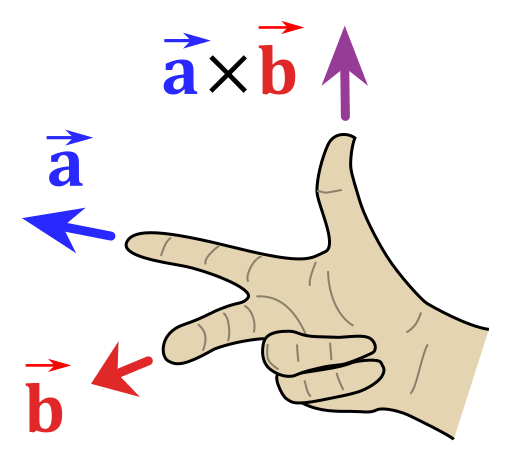
\includegraphics[width=\textwidth]{images/right hand rule cross product.png}\label{img:wikimedia-rhr-cross-product}
      \end{minipage}
    \end{defn}
\end{framed}
\noindent Note: The cross product is only defined in $\mathbb{R}^3$! It does not generalize to other dimensions. Also, some people call the cross product an \emph{external product}.

\begin{ex}
Compute the following:
	\begin{multicols}{3}
    \begin{enumerate}
    	\item $\ii \times\jj $
        \item $\jj \times\ii $
        \item $(2\kk )\times(-\jj )$
    \end{enumerate}
    \end{multicols}
\end{ex}

\vfill

\pagebreak 

\begin{ex}\label{ex:standard-unit-vec-cross-products}
    Cross products of standard unit vectors?
\end{ex}

\vspace{2in}

\begin{ex}
    How are $\vec{u}\times\vec{v}$ and $\vec{v}\times\vec{u}$ related?
\end{ex}

\vspace{2in}

\begin{ex}
    If $\vec{u}$ and $\vec{v}$ are parallel, then\bigskip
    \[\hspace{-5in}\vec{u}\times\vec{v}=\]
\end{ex}

\vspace{.5in}

\begin{ex}
    For any vector $\vec{v}$, we have $\vec{v}\times\vec{v}=$
    \bigskip
\end{ex}
\vspace{.5in}

\begin{thm}[Cross product properties]\label{thm:cross-prod-props}
    Let $\vec{u}, \vec{v}, \vec{w}$ be vectors in $\mathbb{R}^3$ and $c$ any scalar. Then
	\begin{enumerate}
    	\item $\vec{u}\times\vec{v}=\phantom{-(\vec{v}\times\vec{u})}$ \hfill{(Antisymmetry)}
    	\item $c(\vec{u}\times\vec{v})=\phantom{ 	
        (c\vec{u})\times\vec{v}=\vec{u}\times(c\vec{v})}$ \hfill{(Associativity with scalars)}
    	\item $(\vec{u}+\vec{v})\times\vec{w}=$ 
    	%\vec{u}\times\vec{w}+\vec{v}\times\vec{w}$
    	\hfill{(Distributive property)}
    	\item $\vec{u}\times(\vec{v}+\vec{w})=$ 
    	%\vec{u}\times\vec{v}+\vec{u}\times\vec{w}$
    	\hfill{(Distributive property)}
	\end{enumerate}
\end{thm}

\pagebreak 
\begin{ex}
    For $\vec{u}=3\ii +2\kk $ and $\vec{v}=-4\ii +5\jj $, use Theorem~\ref{thm:cross-prod-props} and Exercise~\ref{ex:standard-unit-vec-cross-products} to compute $\vec{u}\times\vec{v}$.
\end{ex}

\vspace{1.8in}

\begin{ex}
    Compute $(\ii +\jj )\times(\jj \times\kk )$.
\end{ex}

\vspace{.7in}

\subsection{Cross product: Geometric interpretation}
\begin{thm}
    Given two nonzero vectors $\vec{u}$ and $\vec{v}$ in $\mathbb{R}^3$, if $\theta$ is the angle between $\vec{u}$ and $\vec{v}$, then \medskip
    \[
        \hspace{-3in}|\vec{u}\times\vec{v}|=\phantom{|\vec{u}|\, |\vec{v}|\,\sin\theta,}
    \]
    \mbox{}\bigskip
    
    \noindent 
    (We'll have $0\le\theta\le\pi$.)
\end{thm}
\begin{ex}
    Suppose $\vec{u}$ and $\vec{v}$ are vectors in $\mathbb{R}^3$ that lie in the $xy$-plane. Suppose $\vec{u}$ has magnitude 3 and $\vec{v}$ has magnitude 4. For $\vec{u}$ and $\vec{v}$ originating at the origin,  if we look down at the $xy$-plane from the positive $z$-axis, we see that $\vec{u}$ points in a direction $\pi/4$ radians counterclockwise from $\vec{v}$. Compute $\vec{u}\times\vec{v}$.
\end{ex}

\pagebreak

\subsection{Interlude: Matrices and determinants}
Now we'll see a way to more efficiently compute cross products. To do so, we'll use matrices.
\begin{defn}[Matrix]
    For positive integers $m$, $n$, a \emph{matrix} is a rectangular array of numbers:
    \bigskip 

    $\displaystyle A = 
    \begin{pmatrix}
        a_{1,1} & a_{1,2} & \dots & a_{1,n} \\ 
        a_{2,1} & a_{2,2} & \dots & a_{2,n} \\ 
        \vdots & \vdots & \ddots & \vdots \\
        a_{m,1} & a_{m,2} & \dots & a_{m,n}
    \end{pmatrix}$
    \bigskip 
    
    A matrix has \emph{rows} (which are horizontal) and \emph{columns} (which are vertical). We refer to a matrix with $m$ rows and $n$ columns as an $m\times n$ (said ``$m$ by $n$'') matrix.
\end{defn}
For our work, we'll deal with determinants of $2\times2$ and $3\times3$ matrices.
\begin{defn}[Determinant]
    Suppose $A$ is a $2\times2$ matrix, so $A=\begin{pmatrix}a&b\\c&d\end{pmatrix}.$ The \emph{determinant} of $A$ is $\det(A)=\phantom{ad-bc.}\hspace{.5in}$ We can also represent this with vertical bars on the matrix:
    \begin{framed}
        \[
            \hspace{-4in}\det(A)=\phantom{|A|=\begin{vmatrix}a&b\\c&d\end{vmatrix}=ad-bc.}
        \]
    \end{framed}
\end{defn}
\begin{ex}
    If $A=\begin{pmatrix}1&4\\-3&-5 \end{pmatrix}$, compute $|A|$.
\end{ex}

\vspace{.5in}

\begin{defn}[Cofactor expansion for determinant]
    Suppose $A$ is a $3\times3$ matrix. %, so $A=\begin{pmatrix}a&b&c\\d&e&f\\g&h&i\end{pmatrix}.$ 
    The \emph{determinant} of $A$ is computed via the following \emph{cofactor expansion}:  
    
    \bigskip
    
    \noindent $\displaystyle
    \det(A) = 
    \begin{vmatrix}a&b&c\\d&e&f\\g&h&i\end{vmatrix}
    =
    \phantom{
        a\begin{vmatrix}e&f\\h&i\end{vmatrix}
        -b\begin{vmatrix}d&f\\g&i\end{vmatrix}
        +c\begin{vmatrix}d&e\\g&h\end{vmatrix}.
    }
    $
\end{defn}
\begin{ex}
    Let $A=\begin{pmatrix}
        2&3&4\\ 
        0&-5&1\\
        -3&2&10
    \end{pmatrix}$.
    Compute $|A|$.
\end{ex}
\pagebreak

\subsection{Cross product: Computational shortcut}
\begin{thm}
    Suppose $\vec{u}=\langle u_1,u_2,u_3\rangle$ and $\vec{v}=\langle v_1,v_2,v_3\rangle$. The  \emph{cross product} of $\vec{u}$ and $\vec{v}$ is 
    \begin{framed}
        \[
            \hspace{-3in}\vec{u}\times \vec{v}=\langle u_1,u_2,u_3\rangle \times \langle v_1,v_2,v_3\rangle = \phantom{\begin{vmatrix}\ii &\jj &\kk \\u_1&u_2&u_3\\v_1&v_2&v_3\end{vmatrix}.}
        \]
    \end{framed}
\end{thm}
\begin{ex}
    Expand $\vec{u}\times\vec{v}$ in terms of $2\times2$ determinants, then multiply it out.
\end{ex}

\vspace{1.3in}

\begin{ex}
Let $\vec{u}=\langle 3,0,2\rangle$ and $\vec{v}=\langle -4,5,0\rangle$.
	\begin{enumerate}
        \item Compute $\vec{u}\times\vec{v}$ using the rule above.
    	\item What is the area of the parallelogram formed by $\vec{u}$ and $\vec{v}$?
        \item What is the area of the triangle formed by $\vec{u}$ and $\vec{v}$?
    	\item Find two unit vectors that are orthogonal to both $\vec{u}$ and $\vec{v}$.
	\end{enumerate}
\end{ex}

\pagebreak 

\subsection{Applications: Area and volume}
A \emph{parallelogram} is a quadrilateral in the plane for which opposite sides are parallel. We can think of a parallelogram is being constructed by two vectors that start at the same point.

\vspace{1in}

The area of such a parallelogram is 
\bigskip

If all of the angles within the parallelogram are right angles, we call it a rectangle. The 3D analogue of a rectangle is a rectangular box. And the 3D analogue of a parallelogram is a parallelopiped!

A \emph{parallelopiped} is a 3D figure made up of 6 faces, each of which is a parallelogram. Opposite faces are parallel. We can think of a parallelopiped as being constructed by three vectors that start at the same point.

\vspace{1.7in}

\begin{thm}
    The volume of a parallelopiped constructed from vectors $\vec{u}$, $\vec{v}$, $\vec{w}$ is
    \[
        |(\vec{u}\times\vec{v})\dotp\vec{w}|.
    \]
\end{thm}
Note: The quantity $(\vec{u}\times\vec{v})\dotp\vec{w}$ is called a \emph{triple scalar product} of $\vec{u}$, $\vec{v}$, and $\vec{w}$.

\begin{ex}
    Find the volume of the parallelopiped formed by the vectors $\vec{u}=\langle 3, 5, -1\rangle$, $\vec{v}=\langle 2, -2, 1\rangle$, and $\vec{w}=\langle 3, 3, 1\rangle$.
\end{ex}

\newlecture

\setcounter{section}{4}
%\def\textbookchapter{Chapter 9: Multivariable and Vector Functions}
\def\coursetopicnumber{I}
\def\textbooksection{9.5} % corresponding textbook section
\def\topic{Lines and Planes in Space} % this is the printed title
\def\shorttopic{Lines and planes} % short topic
\def\textbookname{Active Calculus} % this is the corresponding textbook
\def\textbooksectionurl{https://activecalculus.org/vector/S-9-5-Lines-Planes.html} % URL for textbook section
\def\handoutday{} % this is the printed date

%%%%%%%%% DOCUMENT CONTENT STARTS BELOW

\thispagestyle{plain}
\topstuff
\section{\topic{} \booklink{}}
\label{sec:lines-and-planes}

\subsection{Vector-valued functions}
In Definition~\ref{defn:position-vector}, we defined a \emph{position vector} as a vector that has its tail at the origin (denoted $O$). We'll often use the variable $\vec{r}$ to represent a position vector. If $P_0=(x_0,y_0,z_0)$ is a point in space, then the position vector that represents the point $P_0$ is $\vec{r}_0=\vec{OP_0}=\phantom{\vec{OP_0}=\langle x_0,y_0,z_0\rangle}$

\vspace{1.5in}

Since we are interested in position, we will typically work in $\mathbb{R}^2$ and $\mathbb{R}^3$. However, note that everything here applies in $\mathbb{R}^n$ for any $n\ge1$.

A vector in 3-space has the form $\vec{r}=\langle x,y,z\rangle$. If we want to introduce motion, we can take $x$, $y$, and $z$ to change over time. In other words, we make them functions of a new variable (often $t$).
\begin{defn}[Vector-valued function, parameter]
    A \emph{vector-valued function} is a function that takes one variable as input and outputs a vector (viewed as a position vector). In $\mathbb{R}^2$ and $\mathbb{R}^3$ a vector-valued function takes the form \medskip 
    \[
    \vec{r}(t)=\phantom{\langle x(t), y(t)\rangle} \hspace{1.6in} \text{ or } \quad \vec{r}(t)=\phantom{\langle x(t),y(t), z(t)\rangle,}\hspace{1.5in}\mbox{}
    \]
    \medskip 
    \\
    for $x(t)$, $y(t)$, $z(t)$ functions of $t$, with $t$ taking values from some interval. We call $t$ a \emph{parameter}. 
\end{defn}
The idea is that as the parameter $t$ changes, we get different position vectors that trace out a \emph{curve} (or path). For this reason, we call a vector-valued function a \emph{parametrization}.

We also say the functions $x(t)$, $y(t)$, $z(t)$ \emph{parametrize} the curve and we have \emph{parametric equations} written as 
\[
    \phantom{x=x(t),\quad y=y(t),\quad z=z(t).}
\]

\pagebreak 

\subsection{Lines in space}
We'll focus on lines here. (More general parametrizations are in Section \ref{sec:vector-valued-functions}.) When we sketch a vector-valued function, instead of drawing vectors, we just draw vector endpoints.

\begin{ex}
    Sketch $\vec{r}(t)=\langle 2,t\rangle$ for $t$ in $[0,3]$.
\end{ex}

\vfill 

\begin{ex}
    Sketch $\vec{r}(t)=\langle t,2\rangle$ for $t$ in $(-\infty,\infty)$.
\end{ex}

\vfill

\noindent Notice that any line can be described with a starting point and a direction!
\medskip

\begin{ex}
    Draw the line which goes through the point $P=(1,-1)$ with direction vector $\vec{v}=\langle 3,2\rangle$. Then draw the line which goes through the point $Q=(3,0)$ with direction vector $\vec{w}=\langle -2,1\rangle$.
\end{ex}
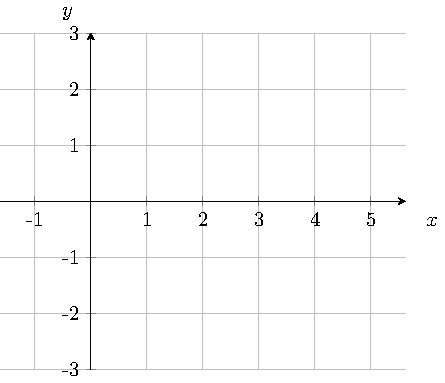
\includegraphics[scale=.8]{tikz-pictures/section-9.2-pic1-axes-for-vectors.pdf} 
\hfill 
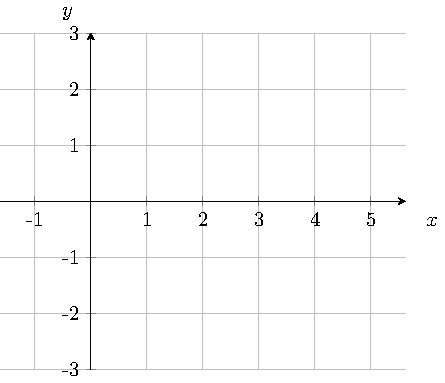
\includegraphics[scale=.8]{tikz-pictures/section-9.2-pic1-axes-for-vectors.pdf}

\begin{framed}
    \begin{thm}[Parametrization of a line]\label{thm:line-param}
        The line through the point $P_0$ (which has corresponding position vector $\vec{r}_0$) in the direction of the vector $\vec{v}$ is parametrized by the vector-valued function
        \[
            \vec{r}(t)=\hspace{.5in}\phantom{\vec{r}_0 + t\vec{v}\quad\quad,} \quad\quad\quad \quad \text{ for $t$ in \phantom{$(-\infty,\infty)$.}}
        \]
        If $\vec{r}_0=\langle x_0,y_0,z_0\rangle$ and $\vec{v}=\langle a,b,c\rangle$, then the parametric equations for this line are 
        \[
            x=\phantom{x_0+at,}\hspace{.3in} \ \quad \quad
            y=\phantom{y_0+bt,}\hspace{.3in} \quad \quad
            z=\phantom{z_0+ct,}\hspace{.3in} \quad \quad \text{ for $t$ in }\phantom{(-\infty,\infty).}
        \]
    \end{thm}
\end{framed}
\pagebreak

Note: To parametrize a line, we need a position vector (for a point on the line) and a direction vector. Since any line contains infinitely many points, and since we can scale the direction vector by any nonzero amount, any line has many different parametrizations!
\begin{ex}
    Find a vector-valued function that describes the line which goes through the points $P=(-1,4)$ and $Q=(3,-7)$. What are the corresponding parametric equations?
\end{ex}

\vfill

\begin{ex}
    Parametrize the line through the point $P=(2,3)$ with slope $-4$.
\end{ex}

\vfill

\begin{ex}
    Parametrize the line in $\mathbb{R}^3$ that goes through the $y$-axis at $y=3$ and through the $z$-axis at $z=-1$.
\end{ex}

\vfill

\pagebreak 

\subsection{Line segments}
In general, the vector-valued function $\vec{r}(t)=\vec{r}_0+t\vec{v}=\langle x_0+at, y_0+bt, z_0+ct\rangle$ with $t$ in the interval $(-\infty,\infty)$ describes a line which extends forever in both directions. If we want to describe just a segment of it, we can restrict the interval of $t$ values.
\begin{ex}
    Consider the vector-valued function $\vec{r}(t)=\langle 3+2t,-t,4\rangle$ with $t$ in the interval $[0,1]$. Describe this line segment. Where does it start and end?
\end{ex}

\vfill

\begin{ex}
    For $P=(1,2,3)$ and $Q=(-2,1,4)$, parametrize the line segment from $P$ to $Q$.
\end{ex}

\vfill\vspace{1.5in}

\begin{thm}[Line segment parametrization]
    In general, the line segment which starts at $P$ and ends at $Q$ is parametrized by
\end{thm}

\vspace{.7in}

\pagebreak

\subsection{Planes in \texorpdfstring{$\mathbb{R}^3$}{3-space}}
Our descriptions of lines can occur in $\mathbb{R}^n$ for any $n$. Now we focus on planes in $\mathbb{R}^3$.
%Just as we described lines in $\mathbb{R}^2$, we can describe planes in $\mathbb{R}^3$.
\begin{ex}
    Consider the plane that contains the point $P=(4,5,6)$ and that is orthogonal to the vector $\vec{n}=\langle 1,2,3\rangle$. If $Q=(x,y,z)$ is in the plane, find an equation that $Q$ satisfies.
\end{ex}

\vfill \vspace{.8in}

In general, if we have a point $P=(x_0,y_0,z_0)$ and a vector $\vec{n}=\langle a,b,c\rangle$, we can draw a plane through $P$ orthogonal to $\vec{n}$. A point $Q=(x,y,z)$ is in the plane precisely when $\vec{n}\dotp\vec{PQ}=0$.

Since $\vec{PQ}=\langle x-x_0,y-y_0,z-z_0\rangle$, we can rewrite this equation as \[\vec{n}\dotp\vec{PQ}=\hspace{5in}\]

\vfill

\begin{framed}
    \begin{thm}[Equation of a plane]
        Given any point $P=(x_0,y_0,z_0)$ and any nonzero vector $\vec{n}=\langle a,b,c\rangle$, the plane in $\mathbb{R}^3$ through $P$ orthogonal to $\vec{n}$ (called a \emph{normal vector}) is described by the equation
        \[
            \phantom{a(x-x_0)+b(y-y_0)+c(z-z_0)=0.}
        \] 
        Alternatively, we can write this as 
        \[
            \phantom{ax+by+cz=d, \text{\quad  where $d=ax_0+by_0+cz_0$}.}
        \]
    \end{thm}
\end{framed}
\begin{ex}
    For the plane given by the equation $2x+3y-4z=5$, determine whether or not the point $P=(1,0,3)$ is in the plane.
\end{ex}
\bigskip \bigskip 

\pagebreak

\begin{ex}
    Find an equation for the plane through the point $P=(-1,2,0)$ that is orthogonal to the vector $\vec{n}=\langle 4,-5,6\rangle$.
\end{ex}

\vspace{.6in}

\subsection{Application: Three (non-colinear) points determine a plane}
\begin{defn}[Colinear, non-colinear]
    Let $P$, $Q$, $R$ be three points. We say $P$, $Q$, and $R$ are \emph{colinear} if they all line on the same line $l$. If there is no such line, we say they are \emph{non-colinear}.
\end{defn}

\vspace{.8in} 

If $P,Q,R$ are non-colinear points in $\mathbb{R}^3$, then they form a triangle $\triangle PQR$. This triangle lies in a plane. Our goal is to find an equation for this plane.

Let $\vec{u}=\vec{PQ}$ and $\vec{v}=\vec{PR}$. Then let $\vec{n}=\vec{u}\times\vec{v}$. Note that $\vec{n}$ is a nonzero vector which is orthogonal to both $\vec{u}$ and $\vec{v}$. Furthermore, $\vec{n}$ is orthogonal to \emph{all} vectors in the plane that contains $\vec{u}$ and $\vec{v}$! Therefore, we have a point ($P$) and normal vector ($\vec{n}$), so we can write down the equation of the plane that contains the triangle $\triangle PQR$.

\begin{ex}
    Find an equation for the plane that contains the points \[P=(1,2,3),\, Q=(1,4,5),\, R=(2,2,4).\]
\end{ex}

\vfill

\pagebreak 

\subsection{Application: Angle between two planes}
Any plane can be described by a point $P=(x_0,y_0,z_0)$ and a nonzero normal vector $\vec{n}=\langle a,b,c\rangle$.

\begin{framed}
    Two planes are \emph{parallel} if their normal vectors are parallel to each other, which is to say that their normal vectors are scalar multiples of each other.
\end{framed}

Note that any plane is parallel to itself.

\begin{framed}
    If two planes are not parallel, then they must intersect. It turns out that they will intersect in a line.
    \bigskip

    The angle between the planes is equal to the angle between their normal vectors.
    \bigskip

    In particular, two planes are \emph{orthogonal} if their normal vectors are orthogonal to each other.
\end{framed}

\vspace{1.3in}

\begin{ex}
    Here are equations for four planes. Determine their normal vectors. Decide which are parallel to each other. Which are orthogonal to each other? %Which go through the origin?
	\begin{multicols}{2}
    \begin{itemize}
    	\item $S_1:$ $3x+y-4z=12$ 
    	\item $S_2: 6x+2y+z=5$ 
    	\item $S_3: x+3y-12z=0$
    	\item $S_4: 60(x-1)+20y-80(z+3)=0$
    \end{itemize}
    \end{multicols}
\end{ex}

\vfill

\begin{ex}
    For the plane $S_1$ in the previous exercise, where does the plane intersect the $x$-axis? Where does it intersect the $y$-axis? The $z$-axis?
\end{ex}

\vfill

\pagebreak

\subsection{Application: Intersection of two planes}
Just like lines, if two planes are not parallel, then they will intersect. Instead of intersecting in a point (like lines do), planes intersect in a line. Here's a trick for finding the line of intersection.

Call the planes $S_1$ and $S_2$. They have normal vectors $\vec{n}_1$ and $\vec{n}_2$. Let $\vec{n}_3=\vec{n}_1\times\vec{n}_2$.
\begin{itemize}
    \item The vector $\vec{n}_3$ is orthogonal to $\vec{n}_1$, so it is in $S_1$. 
    \item The vector $\vec{n}_3$ is orthogonal to $\vec{n}_2$, so it is in $S_2$.
\end{itemize}
Therefore $\vec{n}_3$ is a direction vector for the line of intersection. To parametrize the line of intersection, all we now need is a point $P$ in the intersection of $S_1$ and $S_2$. We can find any such point $P$ by solving the equations for $S_1$ and $S_2$ simultaneously.

\begin{ex}
    Here are two planes: $S_1: x+2y+z=5 \quad \text{ and } \quad S_2: 2x+y-z=7.$ 
    \noindent Are they parallel? If not, find the angle between them and parametrize their line of intersection.
\end{ex}

\vfill

\noindent 
(Here's a shortcut to parametrize the line of intersection of two planes without using normal vectors or cross products. If you can find two points that are each in both planes $S_1$ and $S_2$, then the line of intersection of the planes is simply the line through those points, which you can parametrize via the method of Theorem~\ref{thm:line-param}.)

\pagebreak 

\subsection{Application: Intersection of a line and a plane}
We'll conclude this section by finding the distance from a point to a plane. To do that, we need to first determine the intersection of a line and a plane. Suppose the line has direction vector $\vec{v}$ and the plane has normal vector $\vec{n}$. We have three scenarios to consider:
\begin{enumerate}
    \item The line is in the plane, so the intersection consists of all points on the line.
    \item The line is not in the plane, but is parallel to the plane, so there are no points of intersection.
    \item The line is not in the plane and is not parallel to the plane, so there is one intersection point.
\end{enumerate}
\vspace{1in}

The first two situations arise when the direction vector $\vec{v}$ lies in the plane. This means $\vec{n}$ is orthogonal to $\vec{v}$, so $\vec{n}\dotp\vec{v}=0$. We can further distinguish between these cases by taking any point $P$ on the line. If $P$ is in the plane, then the entire line is in the plane. If $P$ is not in the plane, then no part of the line is in the plane.

The third situation arises when $\vec{v}$ does not lie in the plane, which occurs exactly when $\vec{n}\dotp\vec{v}\ne0$. In this case, we can find the point of intersection of the line and plane. Since $\vec{r}(t)=\langle x(t),y(t),z(t)\rangle$, we plug $x=x(t)$, $y=y(t)$, $z=z(t)$ into the equation of the plane, solve for $t$, and then see where we are on the line at that $t$-value.

\begin{ex}
    Find the point of intersection of the line parametrized by $\vec{r}(t)=\langle 1,2+3t,4-5t\rangle$, for $t$ in $(-\infty,\infty)$, and the plane given by the equation $3x-2y-z=5$.
\end{ex}

\vfill

\subsection{Application: Distance from a point to a plane}
We can use the intersection point from above to compute the distance from a point to a plane.

\begin{thm}[Distance from a point to a plane]
    Given a point $P$ and a plane with a nonzero normal vector $\vec{n}$, parametrize the line through $P$ with direction vector $\vec{v}=\vec{n}$. Since $\vec{n}\dotp\vec{v}=\vec{n}\dotp\vec{n}\ne0$, this line intersects the plane at a point. Call that point $Q$. The distance from $P$ to the plane is the distance from $P$ to $Q$, which is $|\vec{PQ}|$.
\end{thm}

\vspace{1in}

\newlecture

\setcounter{section}{5}
%\def\textbookchapter{Chapter 9: Multivariable and Vector Functions}
\def\coursetopicnumber{I}
\def\topic{Vector-Valued Functions} % this is the printed title
\def\shorttopic{Vector-valued functions} % short topic
\def\textbookname{Active Calculus} % this is the corresponding textbook
\def\shorttextbookname{AC} % this is the short name for the book
\def\textbooksection{9.6} % corresponding textbook section
\def\textbooksectionurl{https://activecalculus.org/vector/S-9-6-Vector-Valued-Functions.html} % URL for textbook section
\def\handoutday{} % this is the printed date


%%%%%%%%% DOCUMENT CONTENT STARTS BELOW

\thispagestyle{plain}
\topstuff

\section{\topic{} \booklink{}}
\label{sec:vector-valued-functions}
\subsection{Domain of a vector-valued functions}
In Section \ref{sec:lines-and-planes}, we saw the definition of a \emph{vector-valued function}, which is a function of the form 
\[
    \vec{r}(t)=\langle x(t),y(t),z(t)\rangle
\] 
where $x(t)$, $y(t)$, $z(t)$ are real-valued functions of $t$.

\begin{defn}[Domain of a vector-valued function]
    The vector-valued function $\vec{r}(t)$ is defined at the values of $t$ for which $x(t)$, $y(t)$, and $z(t)$ are all defined. Thus, the \emph{domain} of $\vec{r}(t)$ is the intersection of the domains of $x(t)$, $y(t)$, and $z(t)$.
\end{defn}

\begin{ex}
    Let $\vec{r}(t)=\left\langle \sqrt{t+3},\dfrac{1}{t}\right\rangle$. Determine the domain of $\vec{r}(t)$.
\end{ex}

\vfill

\subsection{Graph of a vector-valued function}
\begin{defn}[Graph of a vector-valued function]
    The \emph{graph} of a vector-valued function $\vec{r}(t)$ is the set of all endpoints of output vectors of $\vec{r}(t)$ viewed as position vectors.
\end{defn}
When graphing, we put arrows on the graphed path to indicate direction of motion. In Section 9.5, we worked with vector-valued functions whose graphs are lines. In this section, we'll focus on other types of graphs.

\begin{ex}
    Let $\vec{r}(t)=\langle \cos(t),\sin(t)\rangle$. Sketch the graph of $\vec{r}(t)$ for $t$ in each of the following intervals.
    \begin{multicols}{2}
    \begin{enumerate}
        \item $[0,2\pi]$.
        \item $[\pi/2,3\pi/2]$.
    \end{enumerate}
    \end{multicols}
\end{ex}

\vfill

\pagebreak 

\begin{ex}
    Sketch the graph of $\vec{r}(t)=\langle 3+\cos(t),4+\sin(t)\rangle$ for $t$ in $[0,2\pi]$.
\end{ex}

\vfill

\begin{ex}
    Sketch the graph of $\vec{r}(t)=\langle 3\cos(t),4\sin(t)\rangle$ for $t$ in $[0,2\pi]$. Name this curve.
\end{ex}

\vfill

\begin{ex}
    Sketch the curve $\vec{r}(t)=\langle \cos(t),\sin(t),t\rangle$ for $0\le t\le 4\pi$. Name this curve.
\end{ex}

\vfill

\pagebreak 

\begin{ex}
    Sketch the curve $\vec{r}(t)=\langle 2\sin(t),3,2\cos(t)\rangle$ for $t$ in $[0,\pi]$.
\end{ex}

\vfill

\begin{ex}
    Write down a vector-valued function whose graph is the top half of a circle of radius 3 centered at $(4,5)$ traveling counterclockwise.
\end{ex}

\vfill 

\subsection{Shifting direction and time}
\begin{prop}[Changing the direction of motion]
    If the parametrization $\vec{r}(t)$, for $t$ in $[a,b]$, traces out a curve, then the same curve is traced out in the opposite direction by the vector-valued function $\vec{r}(-t)$, for $t$ in $[-b,-a]$.
\end{prop}

\begin{ex}
    Write down a vector-valued function whose graph is the top half of a circle of radius 3 centered at $(4,5)$ traveling clockwise.
\end{ex}

\vfill

\begin{ex}
    Parametrize one revolution along the unit circle starting at $(1,0)$, moving clockwise.
\end{ex}

\vfill

\pagebreak

\begin{ex}
    Parametrize one revolution along the unit circle counter-clockwise, but make it so that it is at the point $(0,1)$ when $t=0$.
\end{ex}

\vfill

We have mostly focused on circular motion here. We can parametrize other types of motion.

\begin{ex}
    Say you have a function $f(x)$. Describe the function $\vec{r}(t)=\langle t, f(t)\rangle$ for $t$ in $[a,b]$.
\end{ex}

\vfill

\begin{ex}
    Write down a parametrization for the path that travels along the parabola $y=x^2$ from the point $(-1,1)$ to the point $(4,16)$.
\end{ex}

\vfill 



\newlecture

\setcounter{section}{6}
%\def\textbookchapter{Chapter 9: Multivariable and Vector Functions}
\def\coursetopicnumber{I}
\def\topic{Derivatives and Integrals of Vector-Valued Functions} % this is the printed title
\def\shorttopic{Calculus of vector-valued functions} % short topic
\def\textbookname{Active Calculus} % this is the corresponding textbook
\def\shorttextbookname{AC} % this is the short name for the book
\def\textbooksection{9.7} % corresponding textbook section
\def\textbooksectionurl{https://activecalculus.org/vector/S-9-7-Vector-Valued-Functions-Derivatives.html} % URL for textbook section
\def\handoutday{} % this is the printed date


%%%%%%%%% DOCUMENT CONTENT STARTS BELOW

\thispagestyle{plain}
\topstuff

\section{\topic{} \booklink{}}
\label{sec:vector-valued-fns-calculus}
Now that we have vector-valued functions, we need to figure out how to do calculus with them. This means understanding limits, derivatives, and integrals. We'll lean heavily on material from Calculus I/II (Math 133/134). %Then we'll think about derivatives geometrically. As an application, we'll learn about projectile motion.

\subsection{Limits of vector-valued functions}
We start with a vector-valued function  
\[
    \vec{r}(t)=x(t)\ii +y(t)\jj +z(t)\kk.
\] 
Note that $\ii$, $\jj$, $\kk$ don't change, so we treat them like constants (which is what they are!).
%\subsection{Limits}
If $\lim\limits_{t\to a}x(t)=l$,\, $\lim\limits_{t\to a}y(t)=m$,\, $\lim\limits_{t\to a}z(t)=n$,\, then 
\begin{align*}
    \lim\limits_{t\to a}\vec{r}(t)
    &=\lim\limits_{t\to a}\left(x(t)\ii +y(t)\jj +z(t)\kk \right)\\
    &=\ii \lim\limits_{t\to a}(x(t))+\jj \lim\limits_{t\to a}(y(t))+\kk \lim\limits_{t\to a}(z(t))\\ \\
    &= % l\ii +m\jj +n\kk 
\end{align*}
%\vspace{.5in}

If any of $\lim\limits_{t\to a}x(t)$, $\lim\limits_{t\to a}y(t)$, $\lim\limits_{t\to a}z(t)$ do not exist, then \phantom{ $\lim\limits_{t\to a}\vec{r}(t)$ does not exist.}
\vspace{.5in}

Important: If $f(t)$ is continuous at $t=a$, then $\lim\limits_{t\to a}f(t) = \phantom{f(a).}$
\medskip 

All of our elementary functions from Calculus I, along with algebraic combinations of them, are continuous wherever they are defined. 

\begin{ex}
    Let $\vec{r}(t)=\left\langle 12\sqrt[3]{t}, 1/t, 2+\ee^t\right\rangle$. Compute $\lim\limits_{t\to 1}\vec{r}(t) $ and $\lim\limits_{t\to 0}\vec{r}(t)$.
\end{ex}

\vspace{2in}

\subsection{Derivatives of vector-valued functions}
The derivative of $\vec{r}(t)$ is 
\[
    \vec{r}\,'(t)=\dd{t}(\vec{r}(t))=\dd{t}\left(x(t)\ii +y(t)\jj +z(t)\kk \right)=\phantom{x'(t)\ii +y'(t)\jj +z'(t)\kk  = \langle x'(t),\, y'(t),\, z'(t)\rangle.}
\]
\bigskip 

\noindent Higher-order derivatives (i.e., second derivative, third derivative, etc.) work exactly as expected!

\begin{ex}
    Let $\vec{r}(t)=\left\langle 12\sqrt[3]{t}, 1/t, 2+\ee^t\right\rangle$. Compute $\vec{r}\,'(t)$ and $\vec{r}\,'(1)$.
\end{ex}

\vspace{1in}

\subsection{Integrals of vector-valued functions}
The indefinite integral of $\vec{r}(t)$ is
\begin{align*}
    \int \vec{r}(t)\dt &= \int\left(x(t)\ii +y(t)\jj +z(t)\kk \right)\dt \hspace{3in} \mbox{}\\ \\
    &= 
\end{align*}
\bigskip

\noindent The definite integral of $\vec{r}(t)$ from $t=a$ to $t=b$ is
\begin{align*}
    \int\limits_a^b \vec{r}(t)\dt &= \int\limits_a^b\left(x(t)\ii +y(t)\jj +z(t)\kk \right)\dt \hspace{3in}\\ \\
    &= \\
\end{align*}

\begin{ex}
    Let $\vec{r}(t)=\left\langle 12\sqrt[3]{t}, 1/t, 2+\ee^t\right\rangle$. Compute $\displaystyle\int\vec{r}(t)\dt$. %and $\displaystyle\int\limits_{1}^{8}\vec{r}(t)\dt$.
\end{ex}

\vfill

\pagebreak 

\subsection{Derivatives visualized: Tangent vectors}
Given a vector-valued function $\vec{r}(t)$, its derivative $\vec{r}\,'(t)$ is called a \emph{tangent vector}. Visually, $\vec{r}(t)$ traces out a curve in space. At any particular time $t=t_0$, the vector $\vec{r}\,'(t_0)$ lies on the tangent line to the point on the curve at $t=t_0$, pointing in the direction of motion at that time.

\begin{ex}
    Let $\vec{r}(t)=\langle \cos(t),\sin(t)\rangle$. Sketch $\vec{r}(t)$ on $[0,2\pi]$ and mark the point on the graph where $t=\pi/6$. Compute $\vec{r}\,'(\pi/6)$, the tangent vector at $t=\pi/6$, and draw it on the graph. Find a parametrization $\vec{L}(t)$ for the corresponding tangent line.
\end{ex}

\vfill 

\begin{ex}
    In the above exercise, our tangent line parametrization meets the circle at $t=0$. How would we modify it so that it meets the circle at $t=\pi/6$?
\end{ex}

\vspace{.6in}

We will be interested in vector-valued functions that describe smooth motion. We want to avoid instantaneous changes of direction, and we want graphs without any sharp points. 
\vspace{.8in}

\begin{defn}[Differentiable]
    We say a function $\vec{r}(t)$ is \emph{differentiable} on an interval of $t$ values if \phantom{$\vec{r}\,'(t)$ is defined everywhere in the interval.}
\end{defn}

\vspace{.5in}

\begin{defn}[Smooth]
    We say a function $\vec{r}(t)$ is \emph{smooth} on an interval of $t$ values if \phantom{$\vec{r}(t)$ is differentiable and $\vec{r}\,'(t)\ne\vec{0}$ on the interval.}
\end{defn}

\vspace{.5in}

\subsection{Position, velocity, acceleration, speed}
If $\vec{r}(t)$ gives the position of an object at time $t$, then $\vec{v}(t)=\vec{r}\,'(t)$ is a \emph{velocity} vector! It points in the direction of motion, and its magnitude is the object's \emph{speed}. In other words, the object's speed at time $t$ is $|\vec{r}\,'(t)|$.

Units? From Calculus I, we know that in general, for a function $f(x)$,
\begin{center}the units of $f'(x)$ are \hspace{3in}\mbox{}\end{center}
\bigskip

Thus, the units of $\vec{r}\,'(t)$ and $|\vec{r}\,'(t)|$ are units of $\vec{r}(t)$ per unit of $t$. (E.g., ft/s.)

Once we have the velocity vector, we can take another derivative to get $\vec{a}(t)=\vec{r}\,''(t)$, the object's \emph{acceleration} vector. Its units are units of $\vec{r}(t)$ per units of $t$ squared. (E.g., ft/s$^2$.)


\begin{ex}
    Let $\vec{r}(t)=\langle 3\cos(t),3\sin(t)\rangle$ represent the position (measured in feet) of an object at time $t$ (measured in seconds).
    \begin{enumerate}
        \item Compute the object's velocity and acceleration vectors at time $t$.
        \item How fast is the object moving at time $t$? Units?
        \item Sketch $\vec{r}(t)$. For $t_0=3\pi/2$, mark the point on $\vec{r}(t)$ with $t=t_0$. Sketch $\vec{v}(t_0)$ and $\vec{a}(t_0)$ at that point.
        \item Is the direction of the acceleration vector realistic?
        \end{enumerate}
\end{ex}
\vfill

\begin{ex}
    Say an object's position is given by the vector-valued function $\vec{r}(t)=\langle 2t,t^2,t-3\rangle$. At what time(s), if any, is the object at the point $(-4,4,-5)$? Parametrize the tangent line at that point.
\end{ex}
\vspace{1in}

\pagebreak 

\subsection{Projectile motion}
Just as we did in Calculus I/II, we can use derivatives and integrals to move back and forth between position, velocity, and acceleration.

\begin{ex}
    Suppose that on Planet X, we have a downward force due to gravity given by 12 feet per second per second. Suppose you stand on a 30-foot tall ladder and launch a rock at an angle of $30^\circ$ above horizontal with an initial velocity of 48 feet per second. Find the object's velocity and position vectors.
\end{ex}

\vfill

\begin{ex}
    Still on Planet X, how high did the rock get? How far did the rock travel horizontally before it hit the ground? How fast was the rock moving when it hit the ground?
\end{ex}
\vfill



\pagebreak 
\subsection{Vector-valued function derivative rules}
Let $\vec{u}(t)$ and $\vec{v}(t)$ be differentiable vector-valued functions, and let $f(t)$ be a differentiable scalar-valued function. Let $\vec{c}$ be a constant vector. Our usual derivative rules work as you'd expect!
\bigskip

\newcommand{\listspace}{\vspace{.2in}}
%\hspace{-.6in}
%\begin{minipage}{.8\textwidth}
%\begin{multicols}{2}
\begin{enumerate}[label=\arabic*.]
    \item $\displaystyle\dd{t}(\vec{c})=$\listspace
    \item $\displaystyle\dd{t}\Big(\vec{u}(t)+\vec{v}(t)\Big)=$\listspace
    \item $\displaystyle\dd{t}\Big(f(t)\,\vec{u}(t)\Big)=$\listspace
    \item $\displaystyle\dd{t}\Big(\vec{u}\big(f(t)\big) \Big)=$\listspace
    \item $\displaystyle\dd{t}\Big(\vec{u}(t)\dotp \vec{v}(t) \Big)=$\listspace
    \item $\displaystyle\dd{t}\Big(\vec{u}(t)\times\vec{v}(t) \Big)=$\listspace
\end{enumerate}
%\end{multicols}
%\end{minipage}
%
\begin{ex}
    For $\vec{r}(t)=\left\langle \ee^t\cos(t),\ee^t\sin(t),3\ee^t\right\rangle$, suppose $\vec{r}(t)$ gives the position of an object at time $t$. Find a formula for the speed of the object at time $t$.
\end{ex}
\vfill
%\vspace{.3in}


\newlecture

\setcounter{section}{7}
%\def\textbookchapter{Chapter 9: Multivariable and Vector Functions}
\def\coursetopicnumber{I}
\def\topic{Arc Length} % this is the printed title
\def\shorttopic{Arc length} % short topic
\def\textbookname{Active Calculus} % this is the corresponding textbook
\def\shorttextbookname{AC} % this is the short name for the book
\def\textbooksection{9.8} % corresponding textbook section
\def\textbooksectionurl{https://activecalculus.org/vector/S-9-8-Arc-Length-Curvature.html} % URL for textbook section
\def\handoutday{} % this is the printed date

%%%%%%%%% DOCUMENT CONTENT STARTS BELOW

\thispagestyle{plain}
\topstuff

\section{\topic{} \booklink{}}
\label{sec:arc-length}
\subsection{Arc length}
Let $\vec{r}(t)$ be a vector-valued function. If we plot $\vec{r}(t)$ from some time $t=a$ to some other time $t=b$, we get a curve. How long is this curve? The answer is the \emph{arc length} of $\vec{r}(t)$ from $t=a$ to $t=b$.

Recall that if $\vec{r}(t)$ represents the position of an object, then $|\vec{r}\,'(t)|$ represents its speed. From Calculus I/II, we know the following:
\begin{itemize}
    \item the definite integral of a velocity function gives net displacement (end position minus start position); and
    \item the definite integral of a speed function gives total distance traveled (think car odometer).
\end{itemize}

Thus, we can compute the arc length of a vector-valued function $\vec{r}(t)$ from $t=a$ to $t=b$ by imagining that we are traveling along the path and then computing the total distance traveled.

\begin{framed}
    \begin{thm}[Arc length]\label{thm:arc-length}
        For the vector-valued function $\vec{r}(t)$ with $a\le t\le b$, the arc length of the graph of $\vec{r}(t)$ is
        \[\phantom{\int\limits_a^b|\vec{r}\,'(t)\dt.}\]
    \end{thm}
\end{framed}
If $\vec{r}(t)=\langle x(t),y(t),z(t)\rangle$ for $a\le t\le b$, then we can write its arc length as
\[
    \phantom{\int\limits_a^b\sqrt{x'(t)^2+y'(t)^2+z'(t)^2}\dt.}
\]

\begin{ex}
    For $\vec{r}(t)=\langle 2\cos(t),2\sin(t),t\rangle$, compute the arc length of the curve for $0\le t\le 2\pi$. What curve is this?
\end{ex}

\vfill

\pagebreak 

For most functions $\vec{r}(t)$, $|\vec{r}\,'(t)|$ is a difficult function to integrate because of the square root. Typically, people use some sort of numerical integration method to compute the arc length with very little error. (You saw some methods in Calculus II, such as right-endpoint sums, midpoint sums, Simpson's Rule, etc.)
\begin{ex}
    Set up an integral to compute the arc length of the graph of $\vec{r}(t)=\left\langle 2t,\ee^t, \sqrt{t}\right\rangle$ for $1\le t\le 2$.
\end{ex}

\vfill

We can approximate the above arc length with something like the following command at \href{https://www.wolframalpha.com}{Wolfram Alpha}:
\begin{center}
    %\href{https://www.wolframalpha.com/input/?i=integral+from+t%3D1+to+t%3D2+of+sqrt%5B4%2Be%5E%282t%29%2B1%2F%284t%29%5D+dt}
    \href{https://www.wolframalpha.com/input/?i=integral+from+t%3D1+to+t%3D2+of+sqrt%5B4+%2B+e%5E%282t%29+%2B+1%2F%284t%29%5D+dt}
    {\tt{integral from t=1 to t=2 of sqrt[4+e\string^(2t)+1/(4t)] dt}}
\end{center}
which returns a value of $\approx 5.1274$.

Sometimes, however, $|\vec{r}\,'(t)|$ cleans up nicely as a function that we can integrate, either with a perfect square under the square root or as an expression easily handled with $u$-substitution. Here's an example.

\begin{ex}
    Find the arc length of $\vec{r}(t)=\left\langle 3t,\dfrac{t^3}{3},\dfrac{\sqrt{6}t^2}{2}\right\rangle$ for $0\le t\le 3$.
\end{ex}

\vfill

\pagebreak 

\subsection{A connection to Calculus II}
In Calculus II (Math 134), you saw a formula for the arc length of the graph of $y=f(x)$ for $a\le x\le b$:
\[
    \phantom{\text{arc length } = \int\limits_a^b\sqrt{1+(f'(x))^2}\dx.}
\]

\vspace{1in}

\begin{ex}
    Use Theorem~\ref{thm:arc-length} to show that the above formula works.
\end{ex}

\vfill


\newlecture
\setcounter{chapter}{9}
\setcounter{section}{0}

\def\coursetopicnumber{II}
\def\textbookchapter{Course Topic II: Multivariable Differentiation}
\def\topic{Functions of Several Variables and Three Dimensional Space} % this is the printed title
\def\shorttopic{Multivariable functions, 3D space} % short topic
\def\textbookname{Active Calculus} % this is the corresponding textbook
\def\shorttextbookname{AC} % this is the short name for the book
\def\textbooksection{9.1B} % corresponding textbook section
\def\textbooksectionurl{https://activecalculus.org/vector/S-9-1-Functions.html} % URL for textbook section
\def\handoutday{} % this is the printed date

\addtocontents{toc}{\bigskip \large \textbookchapter \normalsize \medskip \par} %% for table of contents
%%%%%%%%% DOCUMENT CONTENT STARTS BELOW


\thispagestyle{plain}
\topstuff
\section{(9.1B) \topic{} \booklink{}}
At the start of the course, we covered Section 9.1A (textbook subsections 9.1.1 -- 9.1.3). We'll now cover Section 9.1B (textbook subsections 9.1.4 -- 9.1.6) before getting into Chapter 10. We shift our attention from vector-valued functions to multivariable functions.

\setcounter{subsection}{3}
\subsection{Traces}
Let $f(x,y)$ be a function of two variables defined on some domain in the $xy$-plane. For each point $(x,y)$ in the domain, we have a point $(x,y,f(x,y))$ in $\mathbb{R}^3$. The \emph{graph} of $f$ is the set of all such points $(x,y,f(x,y))$. We often write this as $z=f(x,y)$.

Typically, the graph of a function $f(x,y)$ is a surface in $\mathbb{R}^3$. We'll look at an example from the textbook.

\begin{example}
    Let $f(x,y)=\dfrac{x^2\sin(2y)}{32}$. A sketch of the graph of $f$, for $0\le x\le 220$ and $0\le y\le 1.5$ is given below.

    {\centering 
    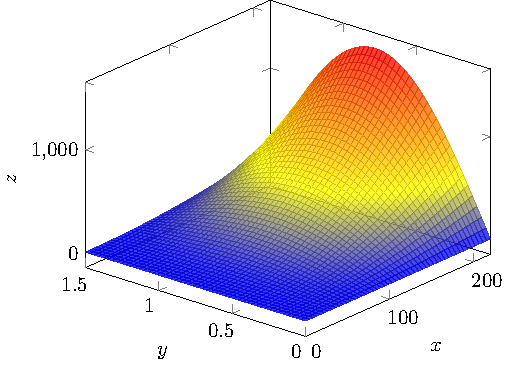
\includegraphics[scale=1]{tikz-pictures/section-9.1-again-pic1-3d-graph-with-traces-1.pdf}\label{img:next-3d-graph}
    \par} 

    \noindent If we intersect this surface with the plane $y=0.6$, we have 
    \[f(x,0.6)=\phantom{\dfrac{x^2\sin(1.2)}{32}}\]
    
    \noindent If we intersect this surface with the plane $x=150$, we have 
    \[f(150,y)=\phantom{\dfrac{150^2\sin(2y)}{32}}\]
    
    The graphs of $z=f(x,0.6)$ and $z=f(150,y)$ are given below.
    
    \pagebreak 
    \mbox{}
    \bigskip 
    
    \begin{center}
        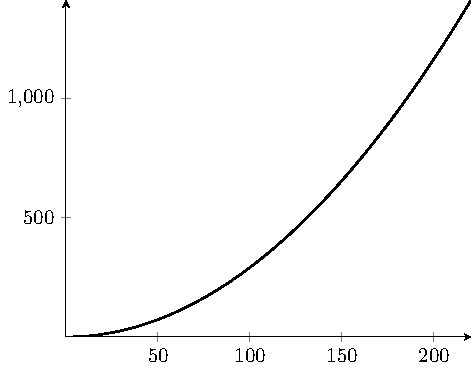
\includegraphics[scale=1]{tikz-pictures/section-9.1-again-pic2-2d-graphs-1.pdf}
        \hfill 
        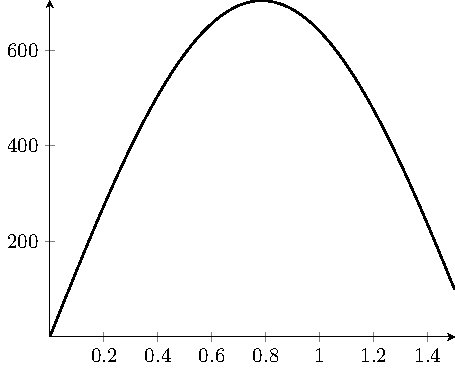
\includegraphics[scale=1]{tikz-pictures/section-9.1-again-pic2-2d-graphs-2.pdf}
    \end{center}
    
    \bigskip 
    
    We can see these graphs on the surface.
    \bigskip 
    
    \begin{center}
        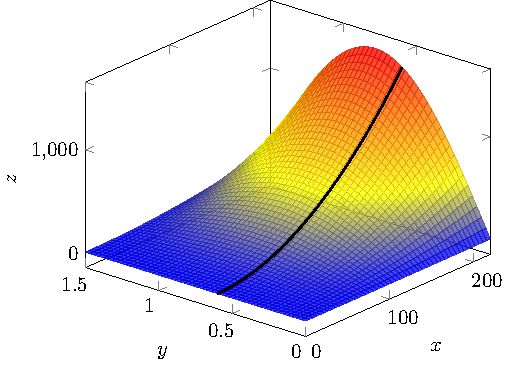
\includegraphics[scale=1]{tikz-pictures/section-9.1-again-pic1-3d-graph-with-traces-2.pdf}
        \hfill
        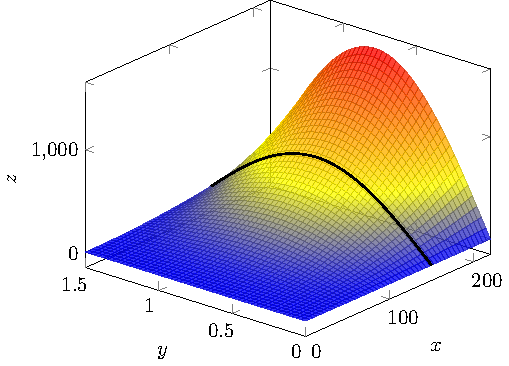
\includegraphics[scale=1]{tikz-pictures/section-9.1-again-pic1-3d-graph-with-traces-3.pdf}\label{img:3d-graph-traces}
    \end{center}
\end{example}

\begin{defn}[Trace]
    An \emph{$x$-trace} of a function $f(x,y)$ is the intersection of the graph of $z=f(x,y)$ with a plane of the form $x=c$, for $c$ constant. In other words, it is the graph of $z=f(c,y)$ in the $yz$-plane.
    
    A \emph{$y$-trace} of a function $f(x,y)$ is the intersection of the graph of $z=f(x,y)$ with a plane of the form $y=c$, for $c$ constant. In other words, it is the graph of $z=f(x,c)$ in the $xz$-plane.
\end{defn}

\pagebreak 

\subsection{Contour maps and level curves}
Here is a side view and an overhead view of some land. The overhead view is called a \emph{topographic map} or \emph{contour map}. Curves on the 3d map are called \emph{contour lines}, and they connect points at the same elevation. On the 2d map, we call them \emph{level curves}
\begin{center}
    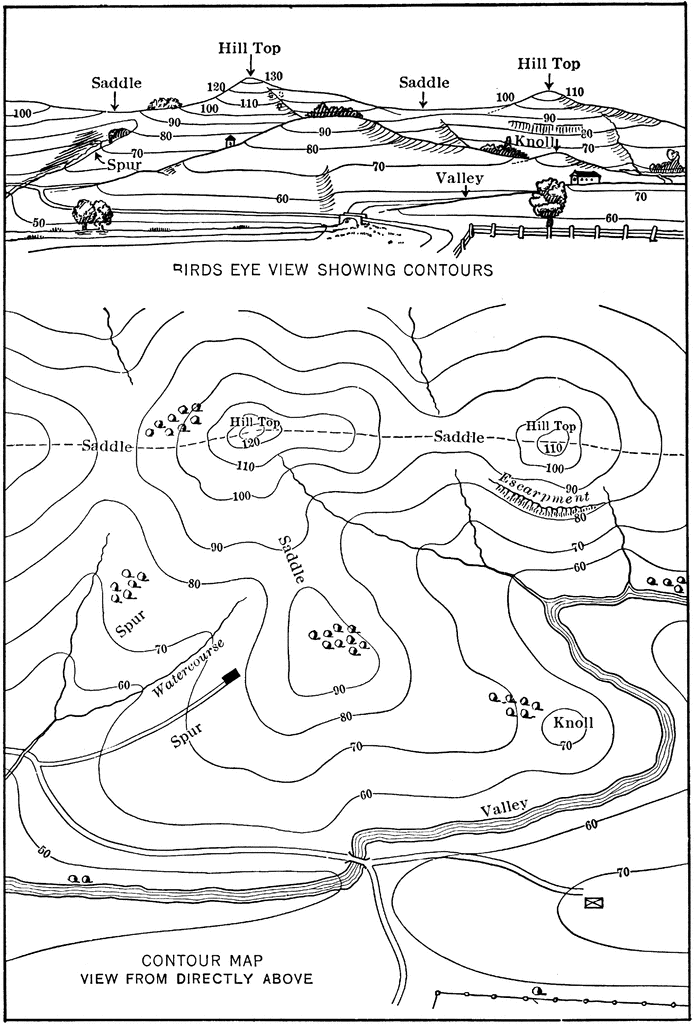
\includegraphics[width=.7\textwidth]{images/contour-map}\label{img:fcit-page-1}
\end{center}

In the context of functions, we can view this map as a portion of $\mathbb{R}^2$. The function $f(x,y)$ that this map represents is the elevation at the point $(x,y)$. In this way, we can visualize a 3D space in a 2D medium.
\vfill\mbox{} 
%\let\thefootnote\relax\footnote{Clipart courtesy FCIT, \href{https://etc.usf.edu/clipart/}{\tt https://etc.usf.edu/clipart/}.}
%\addtocounter{footnote}{-1}\let\thefootnote\svthefootnote
\pagebreak 

Here's another example.
\begin{center}
    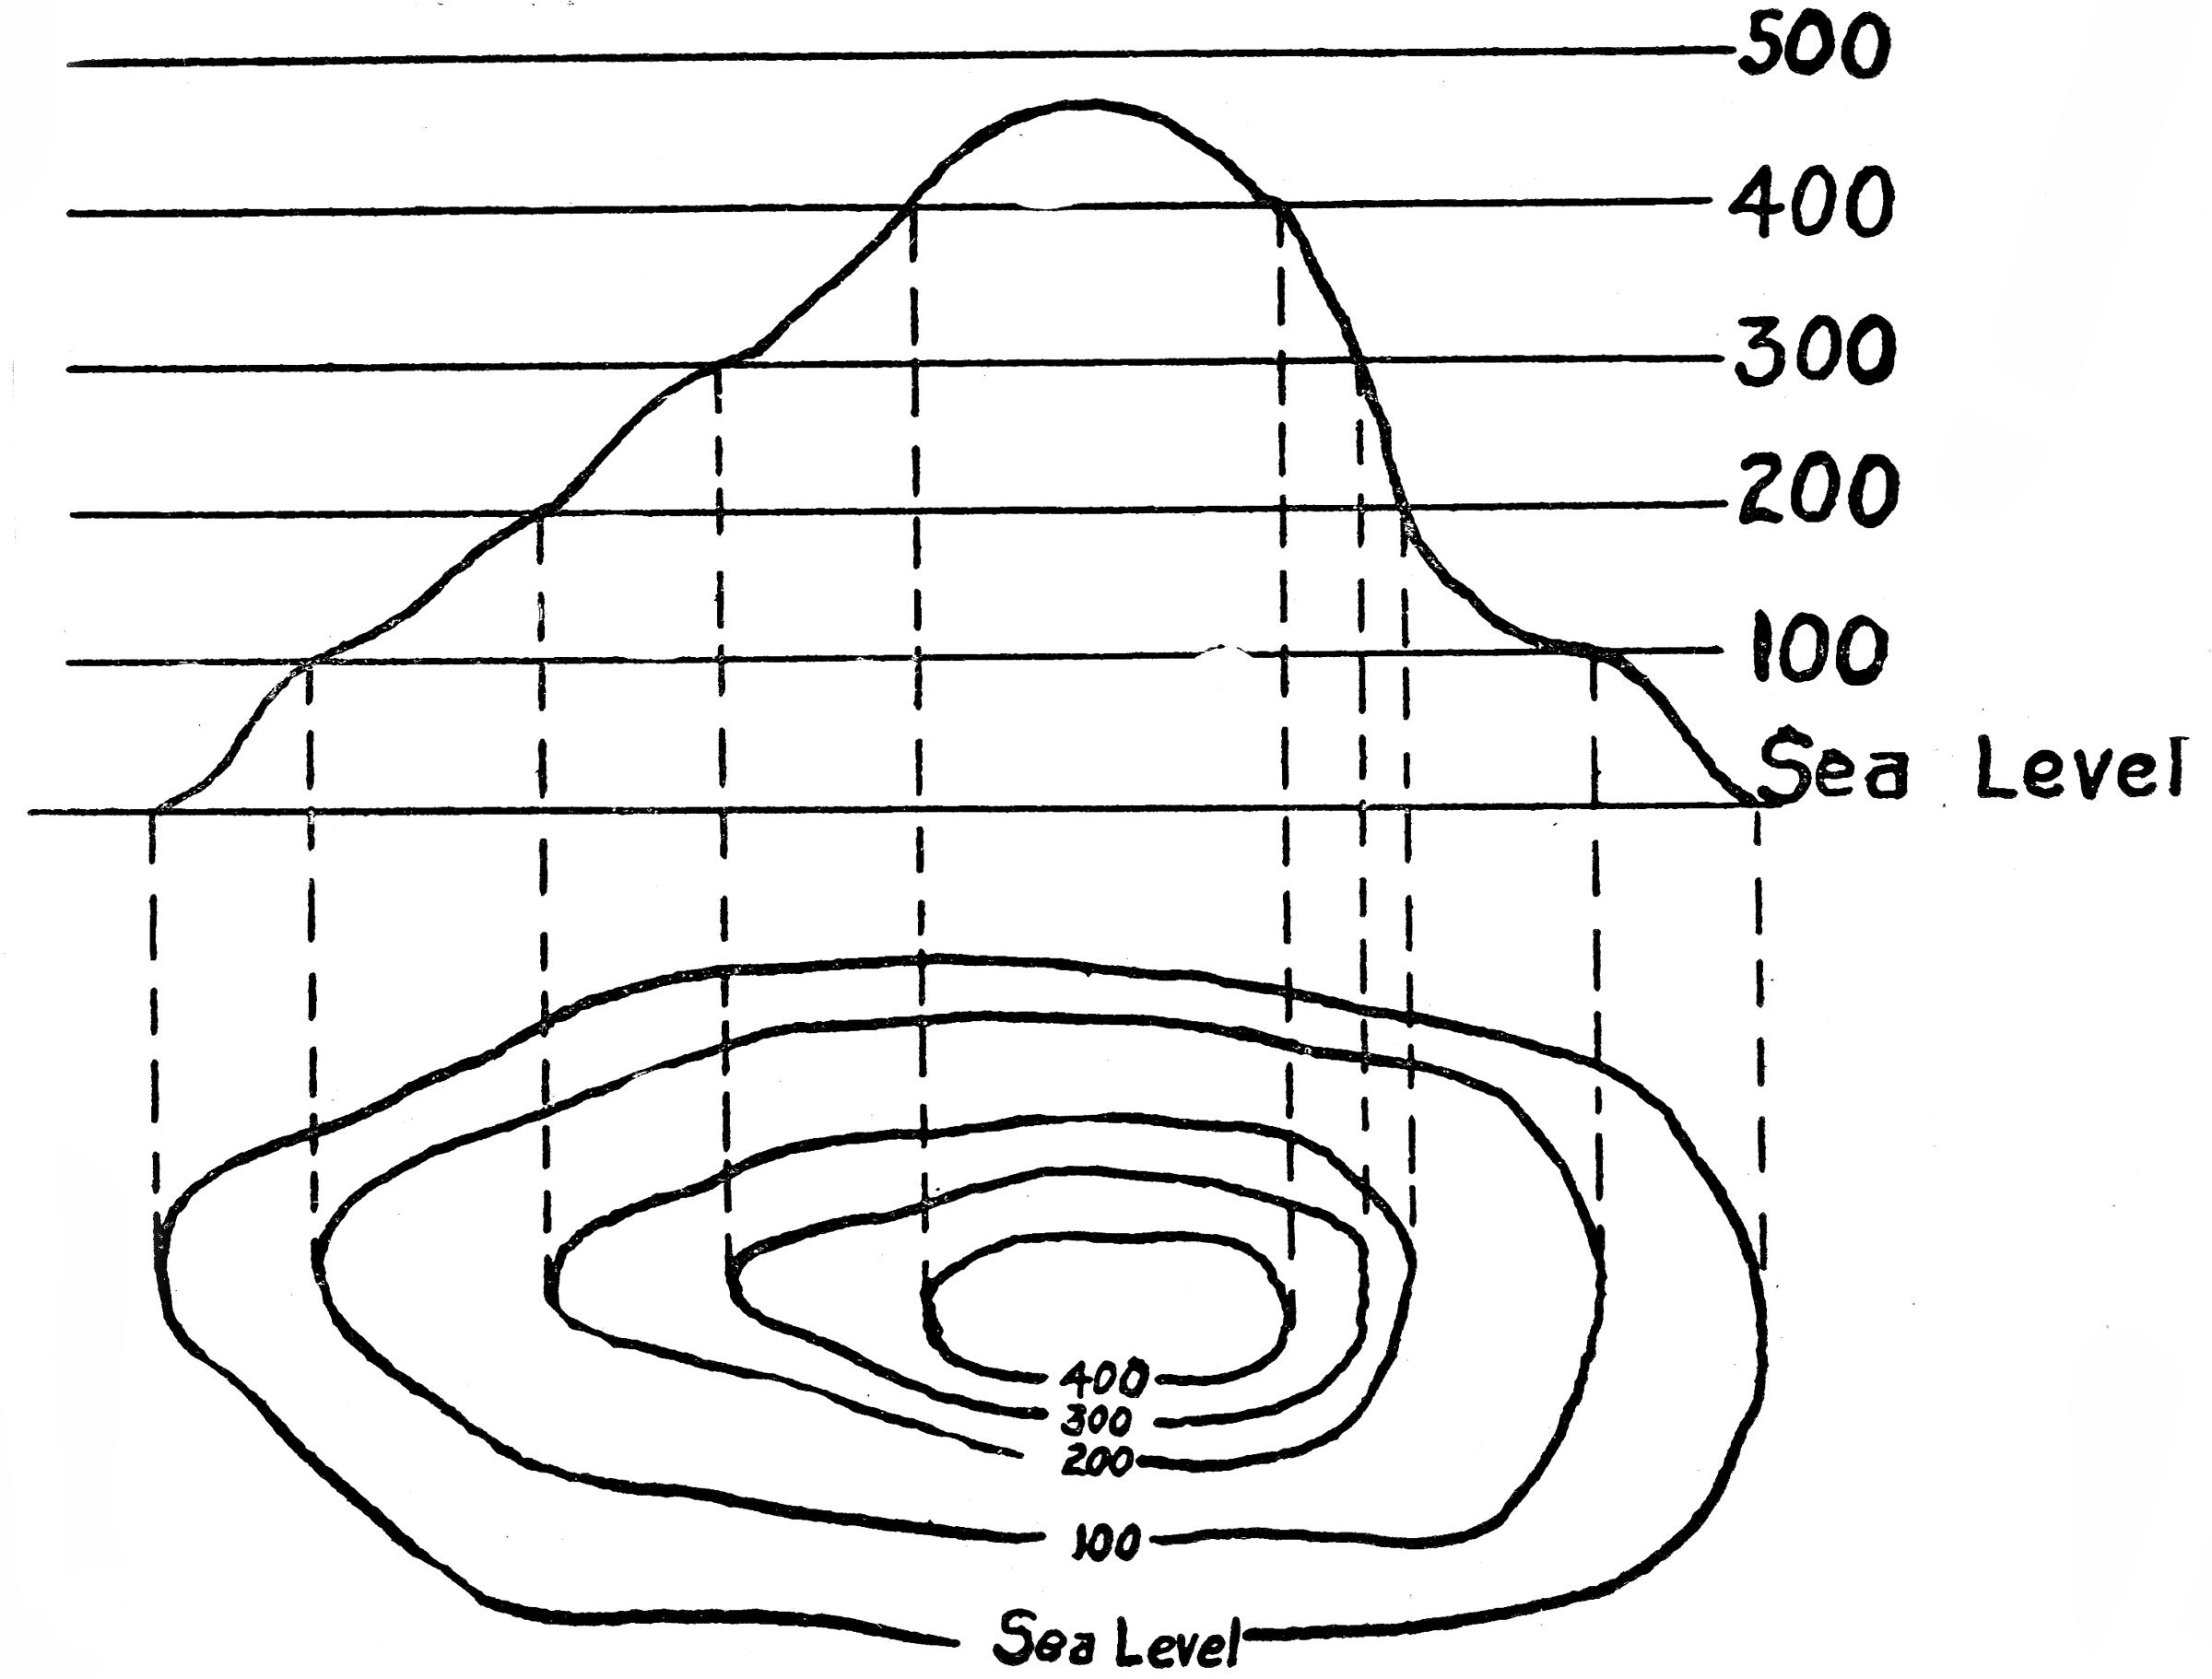
\includegraphics[width=.6\textwidth]{images/topo-map.png}\label{img:fcit-page-2}
\end{center}
\begin{ex}
    Identify major features in the topographic map below.
\end{ex}

\vfill

\begin{center}
    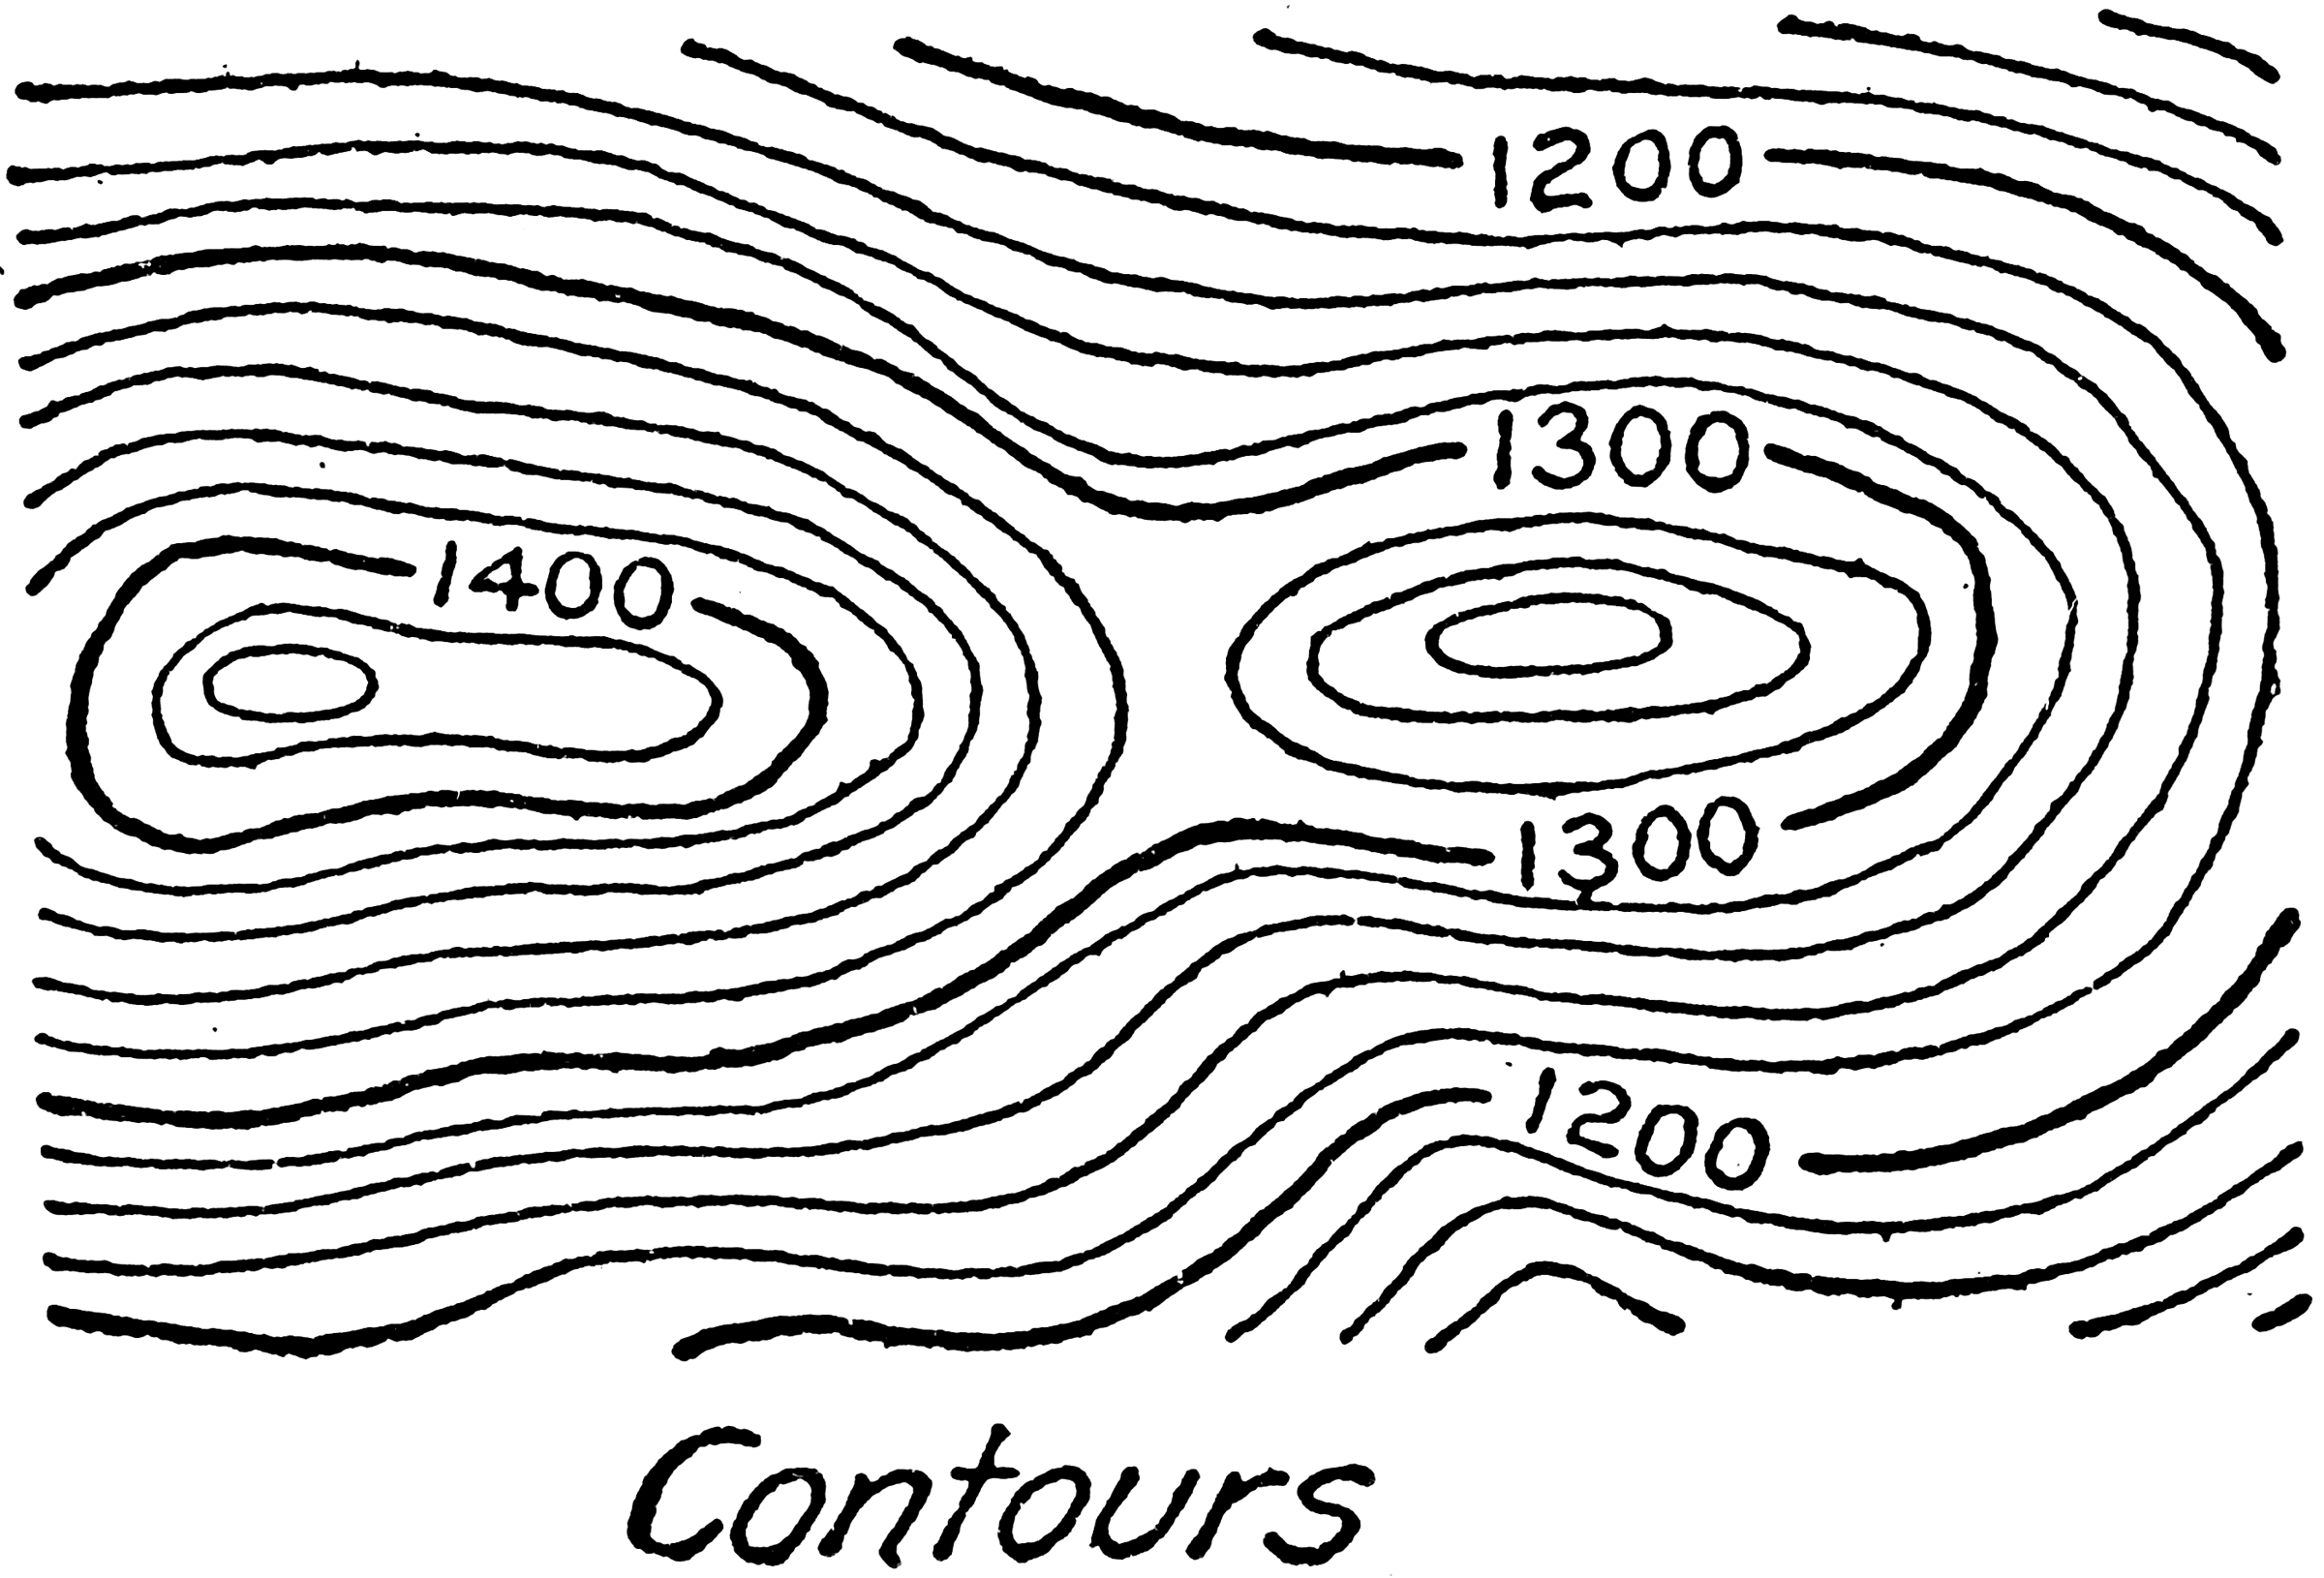
\includegraphics[width=.8\textwidth]{images/topo-map2.png}
\end{center}
\vfill\mbox{} 
%\let\thefootnote\relax\footnote{Clipart courtesy FCIT, \href{https://etc.usf.edu/clipart/}{\tt https://etc.usf.edu/clipart/}.}
%\addtocounter{footnote}{-1}\let\thefootnote\svthefootnote

\pagebreak 

\begin{defn}
    A \emph{level curve} of function $f(x,y)$ is the graph of $f(x,y)=c$ for a constant $c$.
\end{defn}
\begin{ex}\label{ex:elliptic-paraboloid}
    For $f(x,y)=x^2+y^2$, write down the equations of the level curves for $c=0,1,2,\dots,9$. What are these graphs?
\end{ex}
\vfill 

{\centering 
    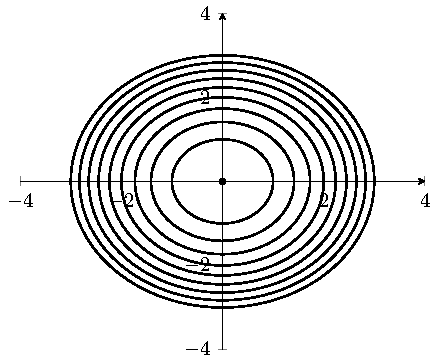
\includegraphics[scale=1]{tikz-pictures/section-9.1-again-pic3-level-curves-elliptic-paraboloid-1.pdf}
\par} 

\begin{center}
    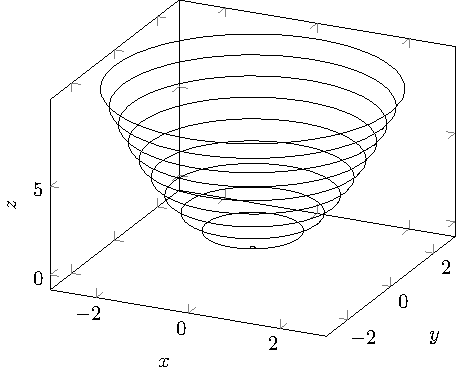
\includegraphics[scale=1]{tikz-pictures/section-9.1-again-pic3-level-curves-elliptic-paraboloid-2.pdf} 
    \hfill 
    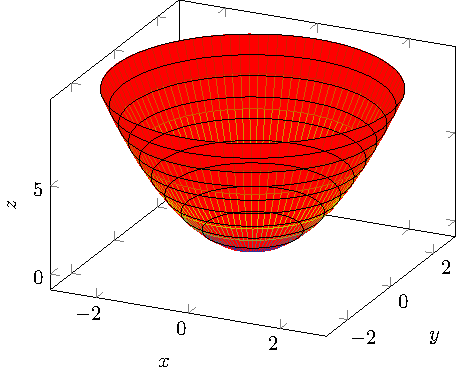
\includegraphics[scale=1]{tikz-pictures/section-9.1-again-pic3-level-curves-elliptic-paraboloid-3.pdf}\label{img:tikz-paraboloid}
\end{center}

\vspace{.5in}

\pagebreak

\begin{ex}\label{ex:cone}
    For $f(x,y)=\sqrt{x^2+y^2}$, write down the equations of the level curves for $c=0,1,2,3,4$. What are these graphs?
\end{ex}

\vfill 

{\centering 
    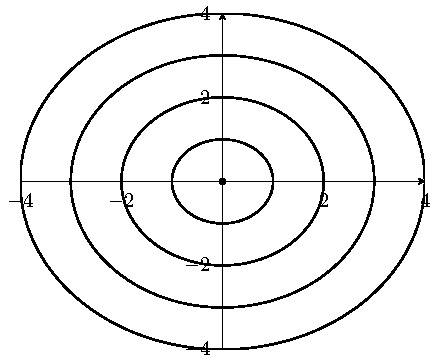
\includegraphics[scale=1]{tikz-pictures/section-9.1-again-pic4-level-curves-cone-1.pdf}
\par} 

\begin{center}
    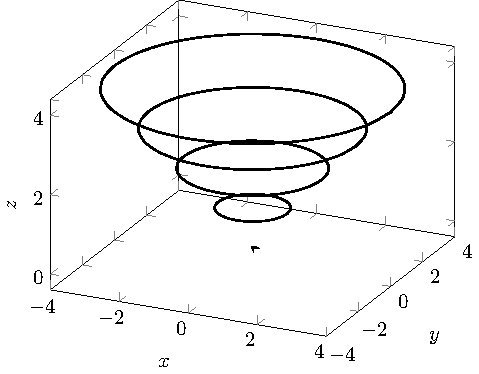
\includegraphics[scale=1]{tikz-pictures/section-9.1-again-pic4-level-curves-cone-2.pdf} 
    \hfill 
    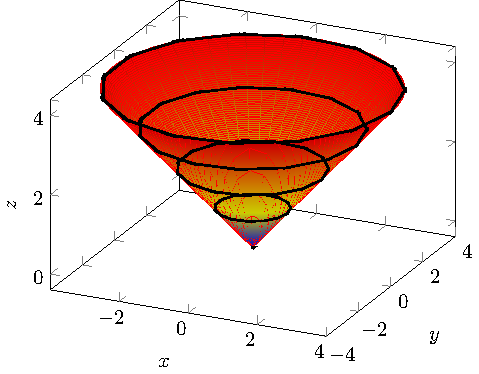
\includegraphics[scale=1]{tikz-pictures/section-9.1-again-pic4-level-curves-cone-3.pdf}\label{img:tikz-cone}
\end{center}

\vspace{.5in}

\pagebreak

\begin{ex}
    For $f(x,y)=-2x-y+6$, write the equations for the level curves for $c=-2,-1,0,1,2$. Sketch the level curves in the $xy$-plane. What does the surface $z=f(x,y)$ look like? Which level curve goes through the point $(x,y)=(4,5)$?
\end{ex}

\vfill\vfill 

\begin{ex}
    Can the level curves of a function cross? Why?    
\end{ex}

\vspace{.5in} 

\begin{ex}\label{ex:shift-bowl}
    We know what the graph of $z=x^2+y^2$ looks like. 
    \begin{enumerate} 
    \item 
    Sketch the graph of $z=(x-1)^2+(y-3)^2$. 
    \item 
    Sketch the graph of $z=4-(x^2+y^2)$.
    \end{enumerate}
\end{ex}

\vfill

\pagebreak

\subsection{A gallery of functions}
In high school geometry, you learned about graphs of low-degree polynomial equations in $x$ and $y$ in $\mathbb{R}^2$.
\begin{itemize} 
    \item Equations of the form $ax+by+c=0$, for constants $a,b,c$, are represented graphically by \emph{lines}. 
    \item Equations of the form $ax^2+bxy+cy^2+dx+ey+f=0$, for constants $a,b,c,d,e,f$, are represented graphically by \emph{conic sections}. These include parabolas, ellipses, and hyperbolas.
\end{itemize}

We now consider low-degree polynomial equations in $x$, $y$, and $z$, and their graphs in $\mathbb{R}^3$. Here are some examples.
\begin{itemize}
    \item The equation $ax+by+cz=d$ graphically is a \emph{plane} with normal vector $\vec{n}=\langle a,b,c\rangle$.
    \item An equation of the form $z=x^2+y^2$ graphically is an \emph{elliptic paraboloid}, or bowl, with vertex at the origin, opening up around the $z$-axis. (Graph given in Exercise \ref{ex:elliptic-paraboloid}.)
    \item An equation of the form $z^2=x^2+y^2$ is an \emph{elliptic cone}, which opens along the positive and negative parts of the $z$-axis. (Top half given in Exercise \ref{ex:cone}.)
    \item An equation of the form $\dfrac{x^2}{a^2}+\dfrac{y^2}{b^2}+\dfrac{z^2}{c^2}=1$ graphically is an \emph{ellipsoid} centered at the origin with radii $a$, $b$, $c$ in the $x-$, $y-$, $z$-directions. When $a=b=c$, we have a sphere.
    \item An equation of the form $z=x^2-y^2$ is a \emph{hyperbolic paraboloid}, or saddle, with flat part at the origin, opening up along the positive and negative parts of the $x$-axis, and opening down along the positive and negative parts of the $y$-axis.
\end{itemize}
As in Exercise \ref{ex:shift-bowl}, we can replace $x,y,z$ with $x-x_0,y-y_0,z-z_0$ to shift a graph. We can also scale variables, swap variables, etc., much in the same way we work with graphs in $\mathbb{R}^2$.

\vfill 

We have seen pictures of planes, elliptic paraboloids, and ellipsoids. Some level curves and a 3D picture of a \emph{hyperbolic paraboloid}, or saddle, which is given by the equation $z=x^2-y^2$, are given below.

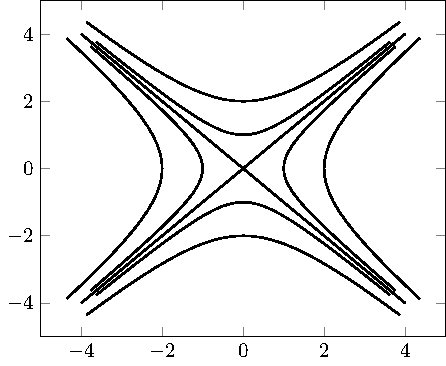
\includegraphics[scale=1]{tikz-pictures/section-9.1-again-pic5-hyperbolic-paraboloid-1.pdf}
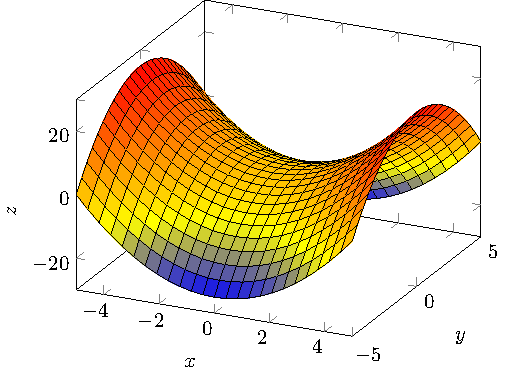
\includegraphics[scale=1]{tikz-pictures/section-9.1-again-pic5-hyperbolic-paraboloid-2.pdf}\label{img:tikz-saddle}


\newlecture
\setcounter{chapter}{10}
\setcounter{section}{0}

%\def\textbookchapter{Chapter 10: Derivatives of Multivariable Functions}
\def\coursetopicnumber{II}
\def\topic{Limits} % this is the printed title
\def\shorttopic{Limits} % short topic
\def\textbookname{Active Calculus} % this is the corresponding textbook
\def\shorttextbookname{AC} % this is the short name for the book
\def\textbooksection{10.1} % corresponding textbook section
\def\textbooksectionurl{https://activecalculus.org/vector/S-10-1-Limits.html} % URL for textbook section
\def\handoutday{} % this is the printed date

%%%%%%%%% DOCUMENT CONTENT STARTS BELOW


\thispagestyle{plain}
\topstuff
\section{\topic{} \booklink{}}
\label{sec:limits}
\subsection{Limits in Calculus I}
Calculus I is all about derivatives of single-variable functions. In order to talk about derivatives, we first need limits!

\begin{defn}[Limit]
    For a function $f(x)$, an $x$ value $a$, and a real number $L$, we say ``the limit of $f(x)$ as $x$ goes to $a$ is $L$,'' written 
    \[
        \phantom{\lim\limits_{x\to a}f(x)=L,}
    \] 
    if the function $f(x)$ gets arbitrarily close to $L$ for all $x$ values sufficiently close to $a$. If no such number $L$ exists, then we say ``the limit of $f(x)$ as $x$ goes to $a$ does not exist (DNE),'' written 
    \[
        \phantom{\lim\limits_{x\to a}f(x) \text{ DNE.}}
    \]
\end{defn}

The key in the definition above is the word ``all.'' The main idea is that $f(x)$ should approach $L$ no matter how one goes to $x=a$. This gives rise to the one-sided limits, $\lim\limits_{x\to a^-}f(x)$ and $\lim\limits_{x\to a^+}f(x)$.

\vspace{.6in}

\begin{ex}
    For $f(x)=\dfrac{|x|}{x}$, compute the following limits:
    %\begin{multicols}{2}
    \begin{enumerate}
        \item $\lim\limits_{x\to 3^-} f(x)$
        \item $\lim\limits_{x\to 3^+} f(x)$
        \item $\lim\limits_{x \to 3}  f(x)$
        \item $\lim\limits_{x\to 0^-} f(x)$
        \item $\lim\limits_{x\to 0^+} f(x)$
        \item $\lim\limits_{x \to 0}  f(x)$
    \end{enumerate}
    %\end{multicols}
\end{ex}

\vfill

\pagebreak 

\begin{defn}[Continuity at a point]
    A function $f(x)$ is \emph{continuous at $x=a$} if
    \begin{multicols}{3}
    \begin{itemize}
        \item \hide{$f(a)$ is defined, }
        \item \hide{$\lim\limits_{x\to a}f(x)$ exists, and}
        \item \hide{$\lim\limits_{x\to a}f(x)=f(a)$.}
    \end{itemize}
    \end{multicols}
\end{defn}

\begin{defn}[Continuity on an interval]
    A function $f(x)$ is \emph{continuous on an interval $I$} if $f(x)$ is continuous at all $x$ values in $I$. (An interval is a subset of $\mathbb{R}$.)
\end{defn}

Basically, this means that the behavior of $f(x)$ near $x=a$ matches with the behavior of $f(x)$ at $x=a$. Graphically, we see this as a connected graph -- one that we can draw without lifting a pen.

\subsection{Limits with multivariable functions}
\begin{defn}[Limit]
    For a function $f(x,y)$, a point $P=(a,b)$, and a real number $L$, we say ``the limit of $f(x,y)$ as $(x,y)$ goes to $(a,b)$ is $L$,'' written 
    \[
        \phantom{\lim\limits_{(x,y)\to(a,b)}f(x,y)=L,}
    \] 
    if the function $f(x,y)$ gets arbitrarily close to $L$ for all points $(x,y)$ sufficiently close to the point $(a,b)$. If no such number $L$ exists, then we say ``the limit of $f(x,y)$ as $(x,y)$ goes to $(a,b)$ does not exist (DNE),'' written
    \[
        \phantom{\lim\limits_{(x,y)\to(a,b)}f(x,y)\text{ DNE}.}
    \]
\end{defn}

As before, the key in the definition above is the word ``all.'' The main idea is that $f(x,y)$ should approach $L$ no matter how one goes to the point $(a,b)$. The difference between now and earlier is that there are so many more ways to approach a point in $\mathbb{R}^2$ than in $\mathbb{R}$!

\vfill

\begin{defn}[Continuity at a point, in a region]
    A function $f(x,y)$ is \emph{continuous at a point $P=(a,b)$} if
    \begin{multicols}{3}
    \begin{itemize}
        \item \hide{$f(a,b)$ is defined,}
        \item \hide{$\lim\limits_{(x,y)\to(a,b)} f(x,y)$ exists, and}
        \item \hide{$\lim\limits_{(x,y)\to(a,b)}f(x,y)=f(a,b)$.}
    \end{itemize}
    \end{multicols}
    A function $f(x,y)$ is \emph{continuous in a region $R$} if $f(x,y)$ is continuous at all points $(x,y)$ in $R$. (A \emph{region} is a subset of $\mathbb{R}^2$.) 
\end{defn}

Basically, this means that the behavior of $f(x,y)$ near $(x,y)=(a,b)$ matches with the behavior of $f(x,y)$ at $(x,y)=(a,b)$. Graphically, we see this as a connected surface, without any jumps or tears.

\pagebreak 

\begin{thm}
    All of our elementary functions (constants, polynomials, rational functions, root functions, trigonometric functions, exponentials, logarithms, inverse trigonometric functions) as well as combinations of them (including addition, subtraction, multiplication, division, exponentiation, and function composition) are continuous wherever they are defined.
\end{thm}

Note: Everything that we're saying here about functions of two variables applies in the same exact way to functions of three variables, of four variables, and so on.
\medskip 

To evaluate $\lim\limits_{(x,y)\to(a,b)}f(x,y)$, if $f(x,y)$ is defined and continuous at the point $(x,y)=(a,b)$, then we can just plug in $x=a$ and $y=b$ and take the result.

\begin{ex}
    Let $f(x,y)=\dfrac{x+y}{x^2+2y^2}$.
    \begin{enumerate}
        \item Evaluate $\lim\limits_{(x,y)\to(3,1)}f(x,y)$. \vfill
        \item Evaluate $\lim\limits_{(x,y)\to(-2,2)}f(x,y)$. \vfill
        \item Are there any points for which we couldn't evaluate the limit here by plugging in?\vfill
    \end{enumerate}
\end{ex}

\subsection{Tricky situations with limits}
There are two situations that make limit evaluation trickier:
\begin{enumerate}
    \item $f(x,y)$ isn't written only in terms of elementary functions. (Often $f(x,y)$ is piecewise-defined, and this includes absolute values.)
    \item $f(x,y)$ isn't defined at $(x,y)=(a,b)$. (This is usually due to division by 0.)
\end{enumerate}
We'll deal mostly with the second case. To handle the limit, we have two techniques.
\begin{itemize}
    \item If we approach the point $(x,y)=(a,b)$ with two different paths in the domain of $f(x,y)$ and get two different results, then the limit does not exist. Note that we can usually evaluate these limits as single-variable limits. We'll see this next, in Section \ref{subsec:different-approaches}.
    \item If we can manipulate $f(x,y)$ algebraically to perform some cancellation, we may be able to directly evaluate the limit. We'll see how to do this in Section \ref{subsec:algebraic-cancellation}.
\end{itemize}

\pagebreak 

\subsection{Different approaches may yield different results}\label{subsec:different-approaches}
If we approach the point $(x,y)=(a,b)$ from two different directions and get two different results, then the limit does not exist.

NOTE: This method will only tell us a limit does not exist. If we get the same result for two different directions, we can't conclude anything. Our primary tool to evaluate a limit is algebraic manipulation. (See the examples that appear after these two examples.)

\begin{ex}
    Let $f(x,y)=\dfrac{x^2+y^2}{x^2+2y^2}$. Compute $\lim\limits_{(x,y)\to(0,0)}f(x,y)$ by computing the limit as $(x,y)$ goes to $(0,0)$ in two different ways: along the $x$-axis; and along the $y$-axis. What can you conclude?
    
    Afterward, compute the limit as $(x,y)$ goes to $(0,0)$ along the line $y=mx$ for constant $m$.
\end{ex}

\vfill

\mbox{} \hfill 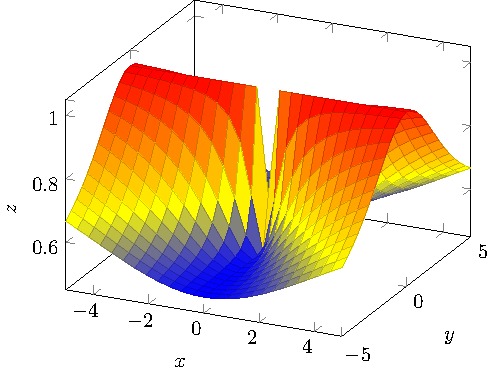
\includegraphics[scale=1]{tikz-pictures/section-10.1-pic1-hole-at-origin.pdf}\label{img:tikz-bad-limit}

\pagebreak 

\begin{ex}
    Let $g(x,y)=\dfrac{x^2y+x^4}{x^4+y^2}$. Compute $\lim\limits_{(x,y)\to(0,0)}g(x,y)$ as $(x,y)$ goes to $(0,0)$ along the line $y=mx$. If that doesn't give a conclusion, try $y=mx^2$.
\end{ex}

\vfill\vfill\vfill

\subsection{Algebra to the rescue}\label{subsec:algebraic-cancellation}
Sometimes, we can use algebraic methods involving factoring and/or conjugates to evaluate limits.
\begin{ex}
    Let $f(x,y)=\dfrac{x^2y-xy}{x-1}$.
    \begin{enumerate}
        \item Evaluate $\lim\limits_{(x,y)\to(0,0)} f(x,y)$.
        \vfill
        \item Evaluate $\lim\limits_{(x,y)\to(1,3)} f(x,y)$.
        \vfill
    \end{enumerate}
\end{ex}

\pagebreak 

\begin{ex}
    Let $g(x,y)=\dfrac{x^2-y^2}{x-y}$. Evaluate $\lim\limits_{(x,y)\to(5,5)}g(x,y)$.
\end{ex}

\vfill

\begin{ex}
    Let $h(x,y)=\dfrac{xy-4y^2}{\sqrt{x}-2\sqrt{y}}$. Evaluate $\lim\limits_{(x,y)\to(4,1)}h(x,y)$.
\end{ex}

\vfill

\pagebreak 

\newlecture
\setcounter{section}{1}

%\def\textbookchapter{Chapter 10: Derivatives of Multivariable Functions}
\def\coursetopicnumber{II}
\def\topic{First-Order Partial Derivatives \& Second-Order Partial Derivatives} % this is the printed title
\def\shorttopic{First-, second-order partials} % short topic
\def\textbookname{Active Calculus} % this is the corresponding textbook
\def\shorttextbookname{AC} % this is the short name for the book
\def\textbooksection{10.2 \& 10.3} % corresponding textbook section
\def\textbooksectionurl{https://activecalculus.org/vector/S-10-2-First-Order-Partial-Derivatives.html} % URL for textbook section
\def\handoutday{} % this is the printed date

%%%%%%%%% DOCUMENT CONTENT STARTS BELOW

\thispagestyle{plain}
\topstuff
\section{First-Order Partial Derivatives \href{\textbooksectionurl}{(book link)}}
\section{Second-Order Partial Derivatives \href{https://activecalculus.org/vector/S-10-3-Second-Order-Partial-Derivatives.html}{(book link)}}
\setcounter{section}{2}

\subsection{Derivatives, graphically}
For a function $f(x)$ and an $x$ value $a$, the \emph{derivative of $f(x)$ at $x=a$} is written as $f'(a)$. We see this graphically as the slope of the tangent line to the graph of $y=f(x)$ at the point $(a,f(a))$. The value of $f'(a)$ tells us how $f(x)$ changes if we're at $x=a$ and increase $x$ a little bit.

In particular, 
\begin{itemize} 
    \item 
    if $f'(a)>0$, then if we're at $x=a$ and we increase $x$, $f(x)$ will \phantom{increase.}
    \item 
    if $f'(a)<0$, then if we're at $x=a$ and we increase $x$, $f(x)$ will \phantom{decrease.}
\end{itemize} 

\pagebreak 

\subsection{Partial derivatives via level curves}
For a function $f(x,y)$ and a point $(a,b)$, the \emph{partial derivative of $f(x,y)$ with respect to $x$ at $(x,y)=(a,b)$} is written as $f_x(a,b)$. The value of $f_x(a,b)$ tells us the rate at which $f(x,y)$ will change if we're at $(x,y)=(a,b)$ and increase $x$ a little bit.

We can interpret the partial derivatives with respect to $x$ in a manner similar to the single variable situation:
\begin{itemize}
    \item if $f_x(a,b)>0$, then if we're at $(x,y)=(a,b)$ and we increase $x$, $f(x,y)$ will \phantom{increase.}
    \item if $f_x(a,b)<0$, then if we're at $(x,y)=(a,b)$ and we increase $x$, $f(x,y)$ will \phantom{decrease.}
\end{itemize}

\bigskip 

For a function $f(x,y)$ and a point $(a,b)$, the \emph{partial derivative of $f(x,y)$ with respect to $y$ at $(x,y)=(a,b)$} is written as $f_y(a,b)$. The value of $f_y(a,b)$ tells us the rate at which $f(x,y)$ will change if we're at $(x,y)=(a,b)$ and increase $y$ a little bit.

We can interpret the partial derivatives with respect to $y$ in a manner similar to the single variable situation:
\begin{itemize}
    \item if $f_y(a,b)>0$, then if we're at $(x,y)=(a,b)$ and we increase $y$, $f(x,y)$ will \phantom{increase.}
    \item if $f_y(a,b)<0$, then if we're at $(x,y)=(a,b)$ and we increase $y$, $f(x,y)$ will \phantom{decrease.}
\end{itemize}

%As we will see in Section \ref{sec:linearization}, just as $f'(a)$ tells us about the slope of a line tangent to the graph of the curve $y=f(x)$ at $x=a$, the partial derivatives $f_x(a,b)$ and $f_y(a,b)$ tell us about slopes on a plane tangent to the graph of the surface $z=f(x,y)$ at $(x,y)=(a,b)$. 
%\pagebreak 

\begin{ex}
    Here are some level curves for $f(x,y)=\dfrac{-x^2+y}{2}.$ The marked points are $P=(-3,12)$ and $Q=(1,10)$.\\
    \mbox{} \hfill 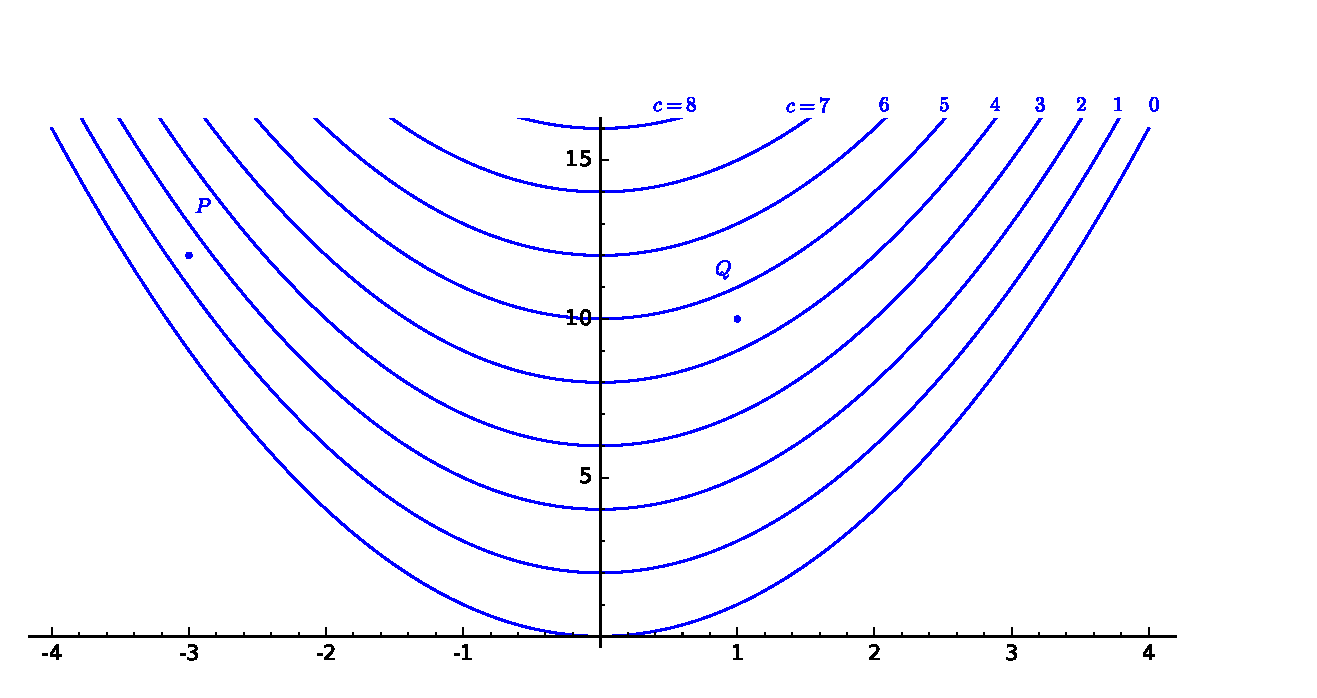
\includegraphics[width=.9\textwidth]{images/partial_deriv_intro.eps}\hfill \mbox{} \label{img:sage-level-curves}
    \\ Decide positive/negative for the following.
    \begin{multicols}{4}
    \begin{enumerate}
        \item $f_x(-3,12)$
        \item $f_y(-3,12)$
        \item $f_x(1,10)$ 
        \item $f_y(1,10)$
    \end{enumerate}
    \end{multicols}
\end{ex}

\pagebreak 



\subsection{Changes in the \texorpdfstring{$x$}{x} and \texorpdfstring{$y$}{y} directions}
\begin{ex}\label{ex:saddle-traces}
    Let $f(x,y)=x^2-y^2$. Below are two views of the graph of $z=x^2-y^2$, a hyperbolic paraboloid (saddle). Two traces are highlighted, corresponding to $y=1$ and $x=1.5$.
    \begin{center}
        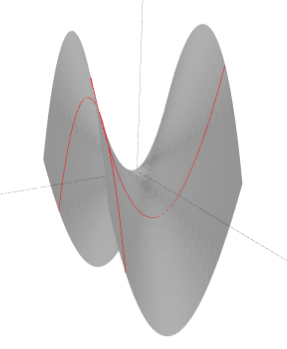
\includegraphics[width=.4\textwidth]{images/saddle1.png}
        \hfill 
        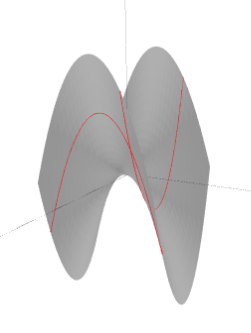
\includegraphics[width=.4\textwidth]{images/saddle2.png}\label{img:sage-saddle}
    \end{center}
    Find the intersection point of the two traces. Call it $P$. Plot the traces in the $xz$- and $yz$-planes and mark $P$ on each. If you're at $P$ and increase $x$, does $f(x,y)$ increase or decrease? If you're at $P$ and increase $y$, does $f(x,y)$ increase or decrease?
\end{ex}

\pagebreak 

\subsection{Derivative notation}
In Calculus I, we defined the \emph{derivative} of $f(x)$ as $f'(x)=$ 
%\[f'(x)=\hspace{1in}\]%\lim\limits_{\Delta x\to 0}\dfrac{f(x+\Delta x)-f(x)}{\Delta x}.\]
\bigskip 

This tells us how $f(x)$ changes as we increase $x$.  

We can then take the \emph{second derivative}, $f''(x)$, which is the derivative of $f'(x)$. Whereas $f'(x)$ tells us about increasing/decreasing, $f''(x)$ tells us about bending (concavity).

And, of course, we can continue to compute derivatives, getting $f'''(x)$, $f''''(x)$, etc.
\vspace{.3in}

In general, then $n$th derivative of $f$ w.r.t.\ $x$ is denoted 
\bigskip 

%\subsection{Notation}
In addition to the prime notation $f'(x)$, we have the \emph{differential operator} $\displaystyle\dd{x}$. It basically means \begin{center}``take the derivative of the following function with respect to the variable $x$.''\end{center}  In other words, 
\[
    \dd{x}f(x) = \hide{f'(x).}
\] 
\medskip 

\noindent Note that the variable in $\dd{x}$ matches the variable in the function. This way of writing derivatives is called \emph{Leibniz notation}.
\begin{ex}
    Write the following in prime notation.
    \begin{multicols}{2}
    \begin{enumerate}
        \item $\displaystyle\dd{t} g(t)$
        \item $\displaystyle\dd{x}\left(\dd{x}f(x)\right)$
        \item $\displaystyle\frac{\dif^2 h}{\dif x^2}$
        \item $\displaystyle\left(\frac{\dif}{\dif y}\right)^2M(y)$
    \end{enumerate}
    \end{multicols}
\end{ex}
If we want to evaluate these functions, we use a vertical bar.
For a function $f(x)$, 
\[
    \left.\dd{x}f(x)\right|_{x=a}=\hide{f'(a).}
\]
Similarly, $\left.\dfrac{\dif^n}{\dif x^n}f(x)\right|_{x=a}=\phantom{f^{(n)}(a)}$
\begin{ex}
    Given $f(x)=\sin(x)+x^2$. Compute $\left.\dfrac{\dif^2}{\dif x^2}f(x)\right|_{x=\pi/2}$
\end{ex}

\pagebreak 

\subsection{Partial derivative notation \& computation}
For a function $f(x,y)$, we can investigate how it changes with respect to $x$ and how it changes with respect to $y$. These rates of change are called \emph{partial derivatives}. Just like the differential operator, we have \emph{partial derivative operators} $\dfrac{\partial}{\partial x}$ and $\dfrac{\partial}{\partial y}$.

The \emph{partial derivative of $f(x,y)$ with respect to $x$}, denoted $f_x(x,y)$ or $\dfrac{\partial}{\partial x}f(x,y)$, is defined as 
\[
    \hspace{-1in}\dfrac{\partial}{\partial x}f(x,y)=\hspace{2in}
\]
%\lim\limits_{\Delta x\to 0}\dfrac{f(x+\Delta x,y)-f(x,y)}{\Delta x}.\]

The \emph{partial derivative of $f(x,y)$ with respect to $y$}, denoted $f_y(x,y)$ or $\dfrac{\partial}{\partial y}f(x,y)$, is defined as 
\[
    \hspace{-1in}\dfrac{\partial}{\partial y}f(x,y)=\hspace{2in}
\]
%\lim\limits_{\Delta y\to 0}\dfrac{f(x,y+\Delta y)-f(x,y)}{\Delta y}.\]

The symbol $\partial$ is generally called ``partial.'' It is also often called ``del.''  Partial derivatives tell us how $f(x,y)$ is changing as we vary $x$ or $y$. \\

{\centering 
    \framebox{
        In practice, we can compute partial derivatives by treating the other variables as constants.
    }
\par}
\begin{ex}
    Let $f(x,y)=x^3-4xy^2+5xy+6$. Compute $\dfrac{\partial}{\partial x}f(x,y)$ and $\dfrac{\partial}{\partial y}f(x,y)$.
\end{ex}

\vfill\vfill

\begin{ex}
    For $f$ above, compute $\dfrac{\partial}{\partial x}\left(\dfrac{\partial}{\partial x}f(x,y)\right)$, $\dfrac{\partial}{\partial y}\left(\dfrac{\partial}{\partial x}f(x,y)\right)$, and $\dfrac{\partial}{\partial x}\left(\dfrac{\partial}{\partial y}f(x,y)\right)$.
    %$\left.\dfrac{\partial}{\partial x}\left(\dfrac{\partial}{\partial y}f(x,y)\right)\right|_{(x,y)=(1,2)}$
\end{ex}

\vfill\vfill\vfill

\pagebreak
%\subsection{Shortcut notation}

We write $f_x(x,y)=\dfrac{\partial}{\partial x}f(x,y)$ and $f_y(x,y)=\dfrac{\partial}{\partial y}f(x,y)$.

We can mimic higher-order derivatives too. If we want to take a partial derivative of $f(x,y)$ with respect to $x$ and then take the partial derivative of that with respect to $y$, we can write that as $f_{xy}(x,y)$.

\vspace{1.5in}

\begin{ex}
    Let $g(x,y)=x(2x+3y)^4+5$. Compute $g_{xx}(x,y)$, $g_{xy}(x,y)$, and $g_{yx}(x,y)$. %, and $g_{yy}(x,y)$. 
    %Then evaluate $\left.\dfrac{\partial^2}{\partial x\partial y}g(x,y)\right|_{(x,y)=(1,\pi)}$
\end{ex}

\vfill 

\begin{thm}[Clairaut's Theorem]
    Let $f$ be a function of more than one variable for which the partial derivatives $f_{xy}$ and $f_{yx}$ are continuous near the point $(a,b)$. Then
    \[
        f_{xy}(a,b) = f_{yx}(a,b).
    \]
\end{thm}

\vspace{1in}

\pagebreak 

\subsection{Computation and interpretation}
\begin{ex}
    Let $f(x,y)=x^2-y^2$. Compute $f_x(1.5,1)$, $f_y(1.5,1)$, $f_{xx}(1.5,1)$, and $f_{yy}(1.5,1)$. How do these relate to Exercise~\ref{ex:saddle-traces}?
\end{ex}

\vfill

\begin{ex}
    Let $f(x,y)=x^3-x^2y+xy^4$. At $(x,y)=(1,-2)$,
    \begin{enumerate}
        \item is $f(x,y)$ increasing or decreasing if we increase $x$ a bit?
        \item is $f(x,y)$ increasing or decreasing if we increase $y$ a bit?
    \end{enumerate}
\end{ex}

\vfill


\newlecture
\setcounter{section}{3}

%\def\textbookchapter{Chapter 10: Derivatives of Multivariable Functions}
\def\coursetopicnumber{II}
\def\topic{Linearization: Tangent Planes and Differentials} % this is the printed title
\def\shorttopic{Linearization: tangent planes} % short topic
\def\textbookname{Active Calculus} % this is the corresponding textbook
\def\shorttextbookname{AC} % this is the short name for the book
\def\textbooksection{10.4} % corresponding textbook section
\def\textbooksectionurl{https://activecalculus.org/vector/S-10-4-Linearization.html} % URL for textbook section
\def\handoutday{} % this is the printed date

%%%%%%%%% DOCUMENT CONTENT STARTS BELOW

\thispagestyle{plain}
\topstuff
\section{\topic{} \booklink{}}
\label{sec:linearization}
\subsection{Single variable}
\subsubsection{Tangent lines}
Given a differentiable function $f(x)$, the equation of the line tangent to the curve $y=f(x)$ at $x=a$ is 
\bigskip 

\noindent $y=T(x)$, for  $T(x)=\phantom{f(a)+f'(a)\cdot (x-a).}$
\vfill

\noindent Reasoning: $T(x)$ is the unique degree-one polynomial such that $T(a)=f(a)$ and $T'(a)=f'(a)$.
\begin{ex}
    Let $f(x)=\sqrt{x}$. Find the equation of the tangent line $y=T(x)$ to the graph of $y=f(x)$ at $x=4$. 
\end{ex}

\vfill

\subsubsection{Linearization}
In particular, $T(x)\approx f(x)$ for $x$-values near $a$. No matter how complicated $f(x)$ is, note that $T(x)$ is a degree-one polynomial in $x$. Therefore, we can use $T(x)$ to approximate $f(x)$ for $x$-values near $a$. For this reason, we also call $T(x)$ a \emph{linearization} (or \emph{linear approximation}) of $f(x)$ at $x=a$.

\begin{ex}
    Continuing the previous exercise, use $T(x)$ to approximate $\sqrt{4.1}$. Based on the graph, is this approximation too big or too small?
\end{ex}

\vfill

\pagebreak 

\subsection{Multiple variables}
\subsubsection{Tangent planes}
Given a differentiable function $f(x,y)$ with continuous first order partial derivatives, the equation of the plane tangent to the surface $z=f(x,y)$ at $(x,y)=(a,b)$ is 
\bigskip 

\noindent $z=T(x,y)$, for  $T(x,y)=\phantom{f(a,b)+f_x(a,b)\cdot (x-a)+f_y(a,b)\cdot (y-b).}$
\vfill

\noindent Reasoning: $T(x,y)$ is the unique degree-one polynomial in $x$ and $y$ such that $T(a,b)=f(a,b)$, $T_x(a,b)=f_x(a,b)$, and $T_y(a,b)=f_y(a,b)$.
\begin{ex}
    Let $f(x,y)=\dfrac{5}{x^2+y^2}$. Find the equation of the tangent plane $z=T(x,y)$ to the graph of $z=f(x,y)$ at $(x,y)=(-1,2)$. Also find a normal vector for this plane.
\end{ex}

\vspace{2.5in}

\subsubsection{Linearization}
In particular, $T(x,y)\approx f(x,y)$ for points near $(a,b)$. No matter how complicated $f(x,y)$ is, note that $T(x,y)$ is a degree-one polynomial in $x$ and $y$. Therefore, we can use $T(x,y)$ to approximate $f(x,y)$ for points near $(a,b)$. For this reason, we also call $T(x,y)$ a \emph{linearization} (or \emph{linear approximation}) of $f(x,y)$ at $(x,y)=(a,b)$.
\begin{ex}
    Continuing the previous exercise, use $T(x,y)$ to approximate $f(-1.05,2.1)$.
\end{ex}

\vfill 

\pagebreak

\subsection{Differentials and change}
\subsubsection{Single variable (Calculus II)}
\begin{ex}
    Evaluate $\displaystyle\int x\sin(x^2)\dx$.
\end{ex}

\vspace{1.2in}

Quantities like $\dif x$ and $\dif u$ are called \emph{differentials}. We think of them as infinitesimally small versions of $\Delta x$ and $\Delta u$.
\medskip 

Differentials help us understand how a small change in the independent variable will affect the dependent variable. In general, if $y=f(x)$, then $\dy=f'(x)\dx$. Thus $\Delta y\approx f'(x)\Delta x$.
\medskip

This relationship actually follows from our linear approximation work. For some $x$-value $a$, we have $y\approx f(a)+f'(a)\cdot(x-a)$, so $y-f(a) \approx f'(a)\cdot(x-a)$.

\vspace{.5in}

\begin{ex}
    Suppose $y=\ln(x)$. Compute $\dy$. Estimate how much $y$ changes when we increase $x$ from $4$ to $4.1$.
\end{ex}

\pagebreak 

\subsubsection{Multivariable (Calculus III)}
Now suppose $z=f(x,y)$. We have two independent variables $x$ and $y$. We can solve for the differential $\dif z$ in terms of $\dx$ and $\dy$ using the linear approximation:
\[
    f(x,y)\approx f(a,b)+f_x(a,b)\cdot(x-a)+f_y(a,b)\cdot(y-b),
\] 
so
\[
    f(x,y)-f(a,b)\approx f_x(a,b)\cdot(x-a)+f_y(a,b)\cdot(y-b).
\]
\bigskip 

\begin{defn}[The differential of a function at a point]
Let $f$ be differentiable at the point $(a,b)$. The change in $z=f(x,y)$ as the independent variables change from $(a,b)$ to $(a+\Delta x, b+\Delta y)$ is denoted $\Delta z$ and is approximated by the \emph{differential} $\dif z$ at $(a,b)$:
\[
    \Delta z\approx \dif z \phantom{= f_x(a,b)\dx + f_y(a,b)\dy.}
\]
\vspace{.6in}
\end{defn}

\begin{ex}
Let $z=f(x,y)=\dfrac{5}{x^2+y^2}$. Compute $\dz$ at $(x,y)=(-1,2)$. Approximate the change in $z$ when $(x,y)$ changes from $(-1,2)$ to $(-0.93, 1.94)$.
\end{ex}

\vfill \vfill\vfill

\noindent Note: If $z=f(x,y)$, we can write $\dif z$ and $\dif f$ interchangeably. They mean the same thing.
\begin{defn}[The differential of a function]
    Given a function $f(x,y)$, the differential $\dif f$ is given by 
    \[
        \dif f = \phantom{f_x(x,y)\dx + f_y(x,y)\dy}
    \]
\end{defn}

\medskip 

\begin{ex}
    Find a function $f(x,y)$ for which $\dif f=(2x+3y)\dx+3x\dy$.
\end{ex}

\vfill

\pagebreak 

\subsection{Linearization, quadratic approximation, and beyond}
\subsubsection{Single-variable}
In Calculus II, you learned about the $n$th degree Taylor polynomial of a function $f(x)$ at $x=a$, which is given by
\[
    T_n(x)=f(a)+\dfrac{f'(a)}{1!}(x-a)+\dfrac{f''(a)}{2!}(x-a)^2+\dfrac{f'''(a)}{3!}(x-a)^3+\dots+\dfrac{f^{(n)}(a)}{n!}(x-a)^n.
\]
To write this, we assume that the first $n$ derivatives of $f(x)$ exist.

This formula comes from the desire to create a degree-$n$ polynomial $T_n(x)$ for which 
\[
    T_n(a)=f(a),\, T_n'(a)=f'(a),\, T_n''(a)=f''(a),\, \dots,\, T_n^{(n)}(a)=f^{(n)}(a).
\]
Geometrically, $T_n(x)$ resembles $f(x)$ for $x$-values near $x=a$. When $n=1$, we have a linear (tangent line) approximation, as seen earlier in this section. When $n=2$, we have a \emph{quadratic approximation}:
\[
    Q(x)=f(a)+f'(a)(x-a)+\dfrac{f''(a)}{2}(x-a)^2.
\]

\begin{ex}
    Find the quadratic approximation for $f(x)=\cos(x)$ at $x=0$.
\end{ex}

\vfill

As $n$ grows, the resemblance between $T_n(x)$ and $f(x)$ gets stronger! As $n$ goes to infinity, we get a Taylor series. For many functions, the function's Taylor series is equal to the function for some interval of $x$-values.

\subsubsection{Multivariable}
As you may expect, all of this translates to the multivariable case. There are Taylor polynomials (and Taylor series) for functions of more than one variable. Rather than writing the general form, we will focus on the \emph{quadratic approximation} $Q(x,y)$ of a function $f(x,y)$ at a point $(a,b)$:
\begin{align*}
    Q(x,y)
    &=f(a,b)+f_x(a,b)\cdot(x-a)+f_y(a,b)\cdot(y-b)\\
    &+\dfrac{f_{xx}(a,b)}{2}\cdot(x-a)^2+\dfrac{f_{xy}(a,b)}{2}\cdot(x-a)\cdot(y-b)+\dfrac{f_{yx}(a,b)}{2}\cdot(x-a)\cdot(y-b)+\dfrac{f_{yy}(a,b)}{2}\cdot(y-b)^2.
\end{align*}
To write this, we assume that the first- and second-order partials of $f$ exist. If the second-order partials are continuous, Clairaut's Theorem says $f_{xy}(a,b)=f_{yx}(a,b)$ and thus
\begin{align*}
    Q(x,y)
    &=f(a,b)+f_x(a,b)\cdot(x-a)+f_y(a,b)\cdot(y-b)\\
    &+\dfrac{f_{xx}(a,b)}{2}\cdot(x-a)^2+f_{xy}(a,b)\cdot(x-a)\cdot(y-b)+\dfrac{f_{yy}(a,b)}{2}\cdot(y-b)^2.
\end{align*}

\pagebreak 

\begin{ex}\label{ex:first-quadratic-approx}
    For $f(x,y)=xy(x-2)(y+6)$ compute the quadratic approximation $Q(x,y)$ of $f(x,y)$ at $(x,y)=(1,-3)$. 
    % This examples connects with an optimization example in 10.7. (1,-3) is a critical point of this function that is, in fact, a local maximum.
\end{ex}


\newlecture

\setcounter{section}{4}
%\def\textbookchapter{Chapter 10: Derivatives of Multivariable Functions}
\def\coursetopicnumber{II}
\def\topic{Chain Rule} % this is the printed title
\def\shorttopic{Chain rule} % short topic
\def\textbookname{Active Calculus} % this is the corresponding textbook
\def\shorttextbookname{AC} % this is the short name for the book
\def\textbooksection{10.5} % corresponding textbook section
\def\textbooksectionurl{https://activecalculus.org/vector/S-10-5-Chain-Rule.html} % URL for textbook section
\def\handoutday{} % this is the printed date

%%%%%%%%% DOCUMENT CONTENT STARTS BELOW

\thispagestyle{plain}
\topstuff
\section{\topic{} \booklink{}}
\label{sec:chain-rule}
\subsection{The chain rule in Calculus I}
Suppose $f$ is a function of $x$, and also suppose $x$ is a function of $t$. We have functions $f(x)$ and $x(t)$. We can compose them to get a new function of $t$: ``$f\circ x$,'' called ``$f$ composed with $x$,'' which is defined as 
\[
    (f\circ x) (t) = \phantom{f(x(t)).}
\] 
In Leibniz notation,
\[
    \dfd{f}{t}=\phantom{\dfd{f}{x}\dfd{x}{t}.}
\]
This gives us the function $f$ in terms of the variable $t$. 

\subsection{The chain rule in Calculus III, one independent variable}
Suppose $f$ is a function of variables $x$ and $y$, and suppose that $x$ and $y$ are each functions of a variable $t$. In other words, we have functions $f(x,y)$, $x(t)$, and $y(t)$.

From our work with differentials in Section~\ref{sec:linearization}, we know that 
\begin{align*}
    \dif f&=\phantom{f_x(x,y)\dx+f_y(x,y)\dy,}\\
    \dx&=\phantom{x'(t)\dt,}\\
    \dy&=\phantom{y'(t)\dt.}
\end{align*}

Subbing $\dx$ and $\dy$ into our expression for $\dif f$, we have
\[
    \dif f=\phantom{f_x(x,y)x'(t)\dt+f_y(x,y)y'(t)\dt.}
\]
This line, along with Leibniz notation, gives us a multivariable Chain Rule for the case of one independent variable ($t$ in this case).

\begin{thm}[Chain Rule with one independent variable]
    Let $f$ be a differentiable function of $x$ and $y$ on its domain (i.e., $f_x$ and $f_y$ exist), where $x$ and $y$ are differentiable functions of $t$ on some interval $I$ (i.e., $x'(t)$ and $y'(t)$ exist). Then 
    \[
        \dfd{f}{t}=\phantom{\pfp{f}{x}\cdot\dfd{x}{t}+\pfp{f}{y}\cdot\dfd{y}{t}.}
    \]
\end{thm}
\noindent \textbf{Note:} This theorem is written for a function $f$ of \emph{two} variables. If $f$ is a function of more than two variables, then the chain rule works exactly as you'd expect! For $f$ is a function of $x$, $y$, and $z$, and if $x$, $y$, and $z$ are functions of $t$, then 
\[
    \dfd{f}{t} = \hspace{4in}
\]

\pagebreak 

The product rule from Calculus I is a special case of the multivariable chain rule!
\begin{ex}
    For $f$ a function of $x$ and $y$, each of which is a function of $t$, suppose $f(x,y)=x\cdot y$. Compute $\displaystyle\dfd{f}{t}$.
\end{ex}

\vspace{1.5in}

\subsection{The chain rule in Calculus III, multiple independent variables}
Suppose $f$ is a function of variables $x$ and $y$, and suppose that $x$ and $y$ are each functions of variables $u$ and $v$. In other words, we have functions $f(x,y)$, $x(u,v)$ and $y(u,v)$.

From our work with differentials in Section~\ref{sec:linearization}, we know that 
\begin{align*}
    \dif f &= f_x(x,y)\dx+f_y(x,y)\dy,\\
    \dif x &= x_u(u,v)\dif u+x_v(u,v)\dif v,\\
    \dif y &= y_u(u,v)\dif u+y_v(u,v)\dif v.
\end{align*}
In other words, 
\[
    \dif f = \phantom{f_x(x,y)\big[x_u(u,v)\dif u+x_v(u,v)\dif v\big]+f_y(x,y)\big[y_u(u,v)\dif u+y_v(u,v)\dif v\big].}
\]
This line, with Leibniz and partial derivative notation, gives us a multivariable chain rule for the case of two independent variables ($u$ and $v$ in this case). Note that $\pfp{u}{v}=0$ and $\pfp{v}{u}=0$.

\begin{thm}[Chain Rule with two independent variables]
    Let $f$ be a differentiable function of $x$ and $y$, where $x$ and $y$ are differentiable functions of $u$ and $v$. Then
    \[
        \pfp{f}{u}= \hspace{2.6in} \text{ and } \hspace{.3in}
        \pfp{f}{v}=\hspace{2.6in}
    \]
\end{thm}

%We'll see how to deal with other scenario using \emph{tree diagrams}.

\begin{ex}
    Let $f(x,y)=3xy-5y^2+4$, \quad $x=2u+v$, \quad and $y=3u-v$. Compute $\displaystyle\pfp{f}{u}$.
\end{ex}

\pagebreak 

\iffalse
\begin{ex}\label{ex:chain-rule-one-var}
Let $f(x)=x^2+3x+4$ and let $x(t)=3t+1$. \\

Compute $(f\circ x)(t)$. Then compute its derivative.
\end{ex}
\vfill

The \emph{chain rule} allows us to calculate its derivative with respect to $t$:
\[
    \hspace{-1in}\dd{t}\Big(f(x(t))\Big) = \phantom{f'(x(t))\cdot x'(t).}
\]
In Leibniz notation, this is written as 
\[
    \hspace{-1in}\dfd{f}{t} = \phantom{\dfd{f}{x} \cdot \dfd{x}{t}.}
\]

This scales up if we have a longer chain of variables. If $f(x)$, $x(t)$, and $t(u)$ are functions, then we can think of $f$ as a function of $u$: $f(x(t(u)))$. Then 
\[
    \hspace{-1in}\dfd{f}{u} = \phantom{\dfd{f}{x}\cdot\dfd{x}{t}\cdot\dfd{t}{u}.}
\]
\begin{ex}
Let $f(x)=x^2+3x+4$ and let $x(t)=3t+1$.
\begin{enumerate}
\item Compute $\dfd{f}{x}$ and $\dfd{x}{t}$. 
\item Multiply them together and compare the result to the derivative in Exercise \ref{ex:chain-rule-one-var}.\end{enumerate}
\end{ex}
\vfill

\pagebreak 

\section{The chain rule in Calculus III}
\subsection{Version 1 -- One independent variable}
Say we have a function $f$ which depends on $x$ and $y$. It could be that $x$ and $y$ both depend on some variable $t$. As $t$ varies, $x$ and $y$ vary, so $f$ varies. Thus, $f$ is a function of $t$, so we can talk about its derivative. I.e., we can talk about $\dfd{f}{t}$.
\begin{ex}
Let $f(x,y)=3xy-5y^2+4$, \quad $x=t^2$, \quad and $y=3t$. \\

Write $f$ as a function of $t$ and compute $\dfd{f}{t}$.
\end{ex}
\vfill

\begin{thm}[Chain Rule with one independent variable]
Let $f$ be a differentiable function of $x$ and $y$ on its domain (i.e., $f_x$ and $f_y$ exist), where $x$ and $y$ are differentiable functions of $t$ on some interval $I$ (i.e., $x'(t)$ and $y'(t)$ exist). Then 
\[
    \dfd{f}{t}=\phantom{\pfp{f}{x}\cdot\dfd{x}{t}+\pfp{f}{y}\cdot\dfd{y}{t}.}
\]
\end{thm}
\noindent \textbf{Note:} This theorem is written for a function $f$ of \emph{two} variables. If $f$ is a function of more than two variables, then the chain rule works exactly as you'd expect! For $f$ is a function of $x$, $y$, and $z$, and if $x$, $y$, and $z$ are functions of $t$, then 
\[\dfd{f}{t} = \hspace{4in}\]
%\vspace{.5in}

\begin{ex}
Let $f(x,y)=3xy-5y^2+4$, \quad $x=t^2$, \quad and $y=3t$. \\

Compute $\pfp{f}{x}$, $\pfp{f}{y}$, $\dfd{x}{t}$, $\dfd{y}{t}$ and use the theorem above to compute $\dfd{f}{t}$.
\end{ex}
\vfill
\pagebreak 
\subsection{Version 2 -- More than one independent variable}
Say we have a function $f$ which depends on $x$ and $y$. It could be that $x$ and $y$ both depend on some variables $u$ and $v$. Thus, $f$ is a function of $u$ and $v$, so we can talk about its partial derivatives with respect to $u$ and $v$. I.e., we can talk about $\pfp{f}{u}$ and $\pfp{f}{v}$.
\begin{ex}
Let $f(x,y)=3xy-5y^2+4$, \quad $x=2u+v$, \quad and $y=3u-v$.\\

Write $f$ as a function of $u$ and $v$, and then compute $\pfp{f}{u}$ and $\pfp{f}{v}$.
\end{ex}
\vfill

\begin{thm}[Chain Rule with two independent variables]
Let $f$ be a differentiable function of $x$ and $y$, where $x$ and $y$ are differentiable functions of $u$ and $v$. Then 
\[\hspace{-1in}\pfp{f}{u}=\phantom{\pfp{f}{x}\cdot\pfp{x}{u}+\pfp{f}{y}\cdot\pfp{y}{u}} \quad \text{ and } \quad \pfp{f}{v}=\phantom{\pfp{f}{x}\cdot\pfp{x}{v} + \pfp{f}{y}\cdot\pfp{y}{v}.}\]
\end{thm}
\noindent \textbf{Note}: We have a similar result when there are more variables. Tree diagrams (next page) will help!
\begin{ex}
Let $f(x,y)=3xy-5y^2+4$, \quad $x=2u+v$, \quad and $y=3u-v$.\\

Compute $\pfp{f}{x}$, $\pfp{f}{y}$, $\pfp{x}{u}$, $\pfp{x}{v}$, $\pfp{y}{u}$, $\pfp{y}{v}$.  Then use the theorem above to compute $\pfp{f}{u}$ and $\pfp{f}{v}$.
\end{ex}
\vfill
\pagebreak
\fi 

\subsection{Tree diagrams}
We can use a \emph{tree diagram} to assist in remembering the chain rule, no matter how many variables we have.

If we have some function (say $a$) that is a function of some variables (say $b$ and $c$), then we write $a$ on one level and write $b$ and $c$ on the level below, connecting $a$ to both $b$ and $c$ with a straight line. We'll mark those lines with the corresponding derivative or partial derivative (in this case $\pfp{a}{b}$ and $\pfp{a}{c}$). Repeat this process with every variable that depends on another variable or variables.

Now, if we have a variable (say $f$) that is in some level above another variable (say $t$), then we can compute the derivative or partial derivative of $f$ with respect to $t$:
\begin{itemize}
    \item For each path from $f$ down to $t$, multiply the derivatives or partial derivatives together. 
    \item Add up the results for every path from $f$ down to $t$.
    \item The result is $\dfd{f}{t}$ (if $t$ is the only variable in its level) or $\pfp{f}{t}$ (if there are other variables in the level of $t$).
\end{itemize}

\begin{ex}
    Say $f$ is a function of $x$, $y$, and $z$. Say each of $x$, $y$, and $z$ is a function of $u$ and $v$.\\
    
    Draw the tree diagram and determine $\pfp{f}{v}$.
\end{ex}

\vfill

\begin{ex}
    Say $A$ is a function of $m$, $m$ is a function of $z$ and $r$, and $z$ and $r$ are functions of $s$ and $j$. Draw the tree diagram and determine $\pfp{A}{j}$.
\end{ex}

\vspace{2in}

\iffalse
\pagebreak 

\section{Implicit differentiation revisited}
Recall that if $x$ and $y$ are related by some implicit equation (like $x^2+y^2=1$), then we can compute $\dfd{y}{x}$ using implicit differentiation. The chain rule gives us a streamlined approach for this calculation.

\begin{ex}
    Suppose we have the equation $F(x,y)=0$ for some function $F$, where $y$ is implicitly defined as a function of $x$. Apply the chain rule to both sides of the equation and solve for $\dfd{y}{x}$.
\end{ex}\vspace{1in}

\begin{thm}
    Let $F$ be differentiable and suppose that $F(x,y)=0$ defines $y$ implicitly as a function of $x$. Then, assuming $F_y\ne0$,
    \[\dfd{y}{x} = \phantom{-\dfrac{F_x}{F_y}}\]
\end{thm}\vspace{1in}

\begin{ex}
    Use the above result to find $\dfd{y}{x}$ given that $x^2+y^2=1$.
\end{ex}
\fi 

\newlecture

\setcounter{section}{5}
%\def\textbookchapter{Chapter 10: Derivatives of Multivariable Functions}
\def\coursetopicnumber{II}
\def\topic{Directional Derivatives and the Gradient} % this is the printed title
\def\shorttopic{Directional derivatives, gradient} % short topic
\def\textbookname{Active Calculus} % this is the corresponding textbook
\def\shorttextbookname{AC} % this is the short name for the book
\def\textbooksection{10.6} % corresponding textbook section
\def\textbooksectionurl{https://activecalculus.org/vector/S-10-6-Directional-Derivative.html} % URL for textbook section
\def\handoutday{} % this is the printed date

%%%%%%%%% DOCUMENT CONTENT STARTS BELOW

\thispagestyle{plain}
\topstuff
\section{\topic{} \booklink{}}
\label{sec:directional-derivative-gradient}
\subsection{Directional derivatives}
For a function $f(x,y)$, thus far we have seen limit definitions for $f_x(x,y)$ and $f_y(x,y)$:
\[
    f_x(x,y)=\lim\limits_{\Delta x\to 0}\dfrac{f(x+\Delta x,y)-f(x,y)}{\Delta x}\quad \text{ and } \quad f_y(x,y)=\lim\limits_{\Delta y\to 0}\dfrac{f(x,y+\Delta y)-f(x,y)}{\Delta y}.
\] 
Our interpretation thus far is that if we are at a point $(a,b)$ in the $xy$-plane, and we move 
\begin{itemize}
    \item eastward (in the positive $x$-direction), then the rate of increase of $f(x,y)$ is 
    \item northward (in the positive $y$-direction), then the rate of increase of $f(x,y)$ is 
\end{itemize}
It turns out that if we know the rate of change of $f$ in these two directions, then we can compute the rate of change of $f$ in ANY direction!

\medskip 

Let $\vec{u}=\langle u_1,u_2\rangle$ be a unit vector that points in the direction we want to move. Suppose we are at the point $P=(a,b)$ and move a distance $h$ in the direction of $\vec{u}$. Our new point $Q$ has coordinates $Q=(a+hu_1,b+hu_2)$. The slope of the secant line connecting these points is 
\[
    \dfrac{\text{rise}}{\text{run}} =     \dfrac{f(Q)-f(P)}{|h\vec{u}|}\hspace{4in}\mbox{}
\]
%\dfrac{f(a+hu_1,b+hu_2)-f(a,b)}{|h\vec{u}|}.\] 
\vspace{1in}

If we let $h$ to go 0, this will give us the slope of the tangent line in the direction of $\vec{u}$ at the point $(a,b)$. In other words, we get the instantaneous rate of change of $f(x,y)$ at $(a,b)$ in the direction $\vec{u}$.
\begin{defn}[Directional Derivative]
    Let $f$ be differentiable at the point $(a,b)$, and let $\vec{u}=\langle u_1,u_2\rangle$ be a unit vector. The \emph{directional derivative of $f$ at $(a,b)$ in the direction of $\vec{u}$} is
    \[
        \D_{\vec{u}}f(a,b)=\lim\limits_{h\to 0}\dfrac{f(a+hu_1,b+hu_2)-f(a,b)}{h}.
    \]
\end{defn}\bigskip

\pagebreak 

\subsection{Computing the directional derivative}
Since the above limit is a single-variable $\frac{0}{0}$ form, we apply l'H\^opital's Rule (from Calculus I):

\begin{align*}
    \D_{\vec{u}}f(a,b)
    &\overset{H}{=}\lim\limits_{h\to0}\dfrac{\frac{\dif}{\dif h}f(a+hu_1,b+hu_2)-\frac{\dif}{\dif h}f(a,b)}{\frac{\dif}{\dif h}h} \\ \\ 
    &= \lim\limits_{h\to0}\dfrac{\frac{\dif}{\dif h} f(x,y)-0}{1} \phantom{\quad\text{ for } x=a+hu_1 \text{ and } y=b+hu_2}
    \\ \\ 
    %&=\lim\limits_{h\to0}\dfrac{f_x(a+hu_1,b+hu_2)\cdot u_1 + f_y(a+hu_1,b+hu_2)\cdot u_2}{1}\\ \\
    &= \\ &
\end{align*}
\vspace{.6in}

\begin{thm}
    Let $f$ be differentiable at the point $(a,b)$, and let $\vec{u}=\langle u_1,u_2\rangle$ be a unit vector. The \emph{directional derivative of $f$ at $(a,b)$ in the direction of $\vec{u}$} is \medskip 
    
    \[
        \D_{\vec{u}}f(a,b)=\phantom{\langle f_x(a,b),f_y(a,b)\rangle\dotp\langle u_1,u_2\rangle.}\hspace{2in}
    \]
\end{thm}
\vspace{1in}

\begin{ex}
    Let $f(x,y)=x^2-7y$. At what rate is $f(x,y)$ changing at the point $(1,2)$ if we move in the direction of the vector $\vec{v}=\left\langle 3,-4\right\rangle$?
\end{ex}

\vspace{2in}

\pagebreak

\subsection{The gradient}
\begin{defn}
    Let $f(x,y)$ be differentiable at the point $(x,y)$. The \emph{gradient} of $f$ at $(x,y)$ is the vector-valued function 
    \[
        \nabla f(x,y)=\phantom{\langle f_x(x,y),f_y(x,y)\rangle = f_x(x,y)\vec{i}+f_y(x,y)\vec{j}.}
    \]
\end{defn}

If $f(x,y,z)$ is differentiable at the point $(x,y,z)$, then
\[
    \nabla f(x,y,z)=\phantom{\langle f_x(x,y,z),f_y(x,y,z),f_z(x,y,z)\rangle = f_x(x,y,z)\vec{i}+f_y(x,y,z)\vec{j}+f_z(x,y,z).}
\]
\medskip 

\begin{ex}
    Let $f(x,y)=3xy+\dfrac{x-2y}{x+y}+5$. Compute $\nabla f(x,y)$.
\end{ex}

\vspace{2in}

\begin{ex}
    How are gradients and differentials related?
\end{ex}

\vspace{1in}

Note that we can use a gradient to compute a directional derivative! For $\vec{u}$ a unit vector, since $\nabla f(x,y)=\langle f_x(x,y),f_y(x,y)\rangle$, \[\D_{\vec{u}} f(a,b) = \hspace{2in}\]% \nabla f(a,b)\dotp \vec{u}.\]
\medskip 

More generally, if $\vec{v}$ is any nonzero vector, then the directional derivative of $f(x,y)$ at $(a,b)$ in the direction of $\vec{v}$ is \[\D_{\vec{v}} f(a,b) = \hspace{2in}\]
\pagebreak 
\begin{ex}
    Consider the surface defined by $z=f(x,y)=x^2+5y^2$. Here is a sketch of its level curves for $c = 0, 5, 10, 15, 20, 25, 30, 35$. The point $P=(5,-1)$ is also marked.
    \bigskip 
    
    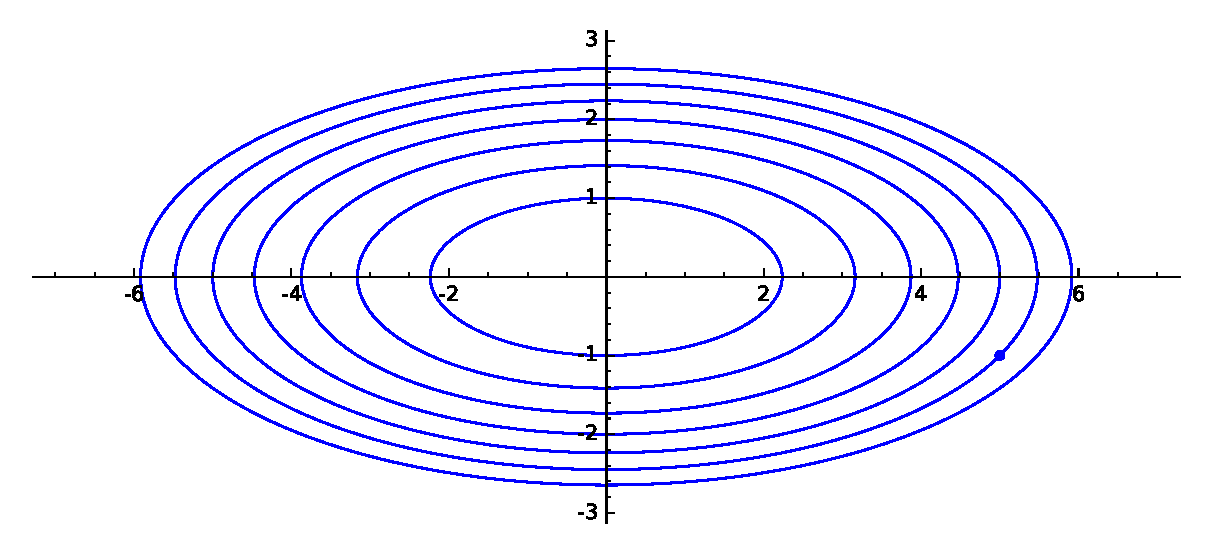
\includegraphics[width=.7\textwidth]{images/circles.eps}\label{img:sage-level-curves-again}
    \begin{enumerate}
        %\item Name the surface.
        \item Sketch the surface.
        \item Find the equation of the level curve through the point $P=(5,-1)$.
        \item Let $\vec{v}_1=\langle 2,-3\rangle$, $\vec{v}_2=\langle 1,1\rangle$, $\vec{v}_3=\langle -1,0\rangle$. 
        Decide if the directional derivatives of $f$ at $P$ in the directions $\vec{v}_1$, $\vec{v}_2$, $\vec{v}_3$ are positive, negative, or zero.
        \item Still with $f(x,y)=x^2+5y^2$, compute $\nabla f(x,y)$.
        \item Compute $\D_{\vec{v}_1}f(P)$, $\D_{\vec{v}_2}f(P)$, and $\D_{\vec{v}_3}f(P)$.
    \end{enumerate}
\end{ex}

\pagebreak 

\subsection{The direction and magnitude of the gradient}
We have seen that the directional derivative of $f$ at $(a,b)$ in the direction of a unit vector $\vec{u}$ is 
\[
    \D_{\vec{u}} f(a,b) = \nabla f(a,b)\dotp \vec{u}.
\] 
This tells us the rate at which $f$ changes if we are at the point $(a,b)$ and move in the direction $\vec{u}$.

Since this involves a dot product, we can think of this in terms of the angle $\theta$ between the vectors $\nabla f(a,b)$ and $\vec{u}$:
\begin{align*}
    \D_{\vec{u}}f(a,b) 
    &= \nabla f(a,b)\dotp\vec{u} \hspace{2in} \\ \\
    & = \\ %& = |\nabla f(a,b)|\, |\vec{u}| \cos\theta,\\
    %& = |\nabla f(a,b)| \cos\theta.
\end{align*}

\noindent Then, since $-1\le \cos\theta \le 1$, the directional derivative $\D_{\vec{u}}f(a,b)$
\begin{itemize}
    \item has its maximum value when $\cos\theta=1$, so when $\theta=$ \\  
    \medskip 
    
    \noindent Therefore the maximum value of $\D_{\vec{u}}f(a,b)$ is \\
    \item has its minimum value when $\cos\theta=-1$, so when $\theta=$ \\  
    \medskip 
    
    \noindent Therefore the minimum value of $\D_{\vec{u}}f(a,b)$ is \\
\end{itemize}

Another important value of $\cos\theta$ is 0. When $\cos\theta=0$, we have $\D_{\vec{u}}f(a,b)=$

\bigskip 

The theorem below summarizes these observations.
\vspace{.5in}

\begin{thm}[Directions of change]\label{thm:dirs-of-change}
    Let $f$ be differentiable at $(a,b)$ with $\nabla f(a,b)\ne \vec{0}$.
    \begin{enumerate}
        \item $f$ has its maximum rate of increase at $(a,b)$ in the direction of the gradient $\nabla f(a,b)$. The rate of change in this direction is $|\nabla f(a,b)|$.\\
        \item $f$ has its maximum rate of decrease at $(a,b)$ in the direction of $-\nabla f(a,b)$. The rate of change in this direction is $-|\nabla f(a,b)|$.\\
        \item The directional derivative is zero in any direction orthogonal to $\nabla f(a,b)$.
    \end{enumerate}
\end{thm}


\pagebreak 

\begin{ex}
    Consider the elliptic paraboloid $z=f(x,y)=x^2+y^2$.
    \begin{enumerate}
        \item In the contour diagram below, mark the point $P=(2,-1)$. Label its level curve as well as the two level curves closest to it. (The level curves are $c=0,1,2,\dots,9$.)
        \item If you are on the paraboloid at the point $(x,y,z)=(2,-1,5)$, in which direction in the $xy$-plane should you move in order to \emph{ascend} on the surface at the maximum rate? What is the rate of change? 
        \item If you are on the paraboloid at the point $(2,-1,5)$, in which direction in the $xy$-plane should you move in order to \emph{descend} on the surface at the maximum rate? What is the rate of change? 
        \item At the point $(2,-1,5)$, in what direction(s) in the $xy$-plane is there no change in the value of $f(x,y)$?
    \end{enumerate}
\end{ex}

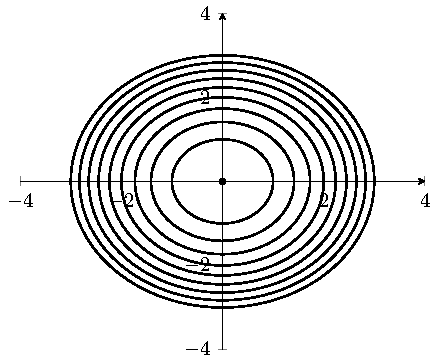
\includegraphics[scale=1]{tikz-pictures/section-9.1-again-pic3-level-curves-elliptic-paraboloid-1.pdf} 
\hfill  
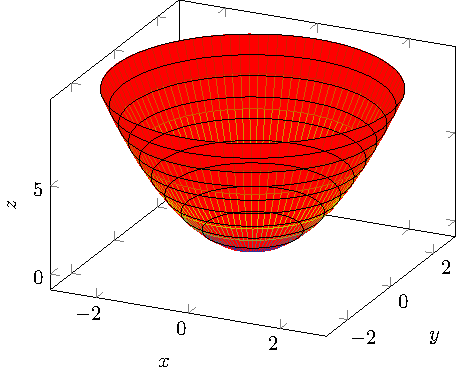
\includegraphics[scale=1]{tikz-pictures/section-9.1-again-pic3-level-curves-elliptic-paraboloid-3.pdf}\label{img:tikz-paraboloid-again}

\pagebreak 
\noindent The third part of Theorem \ref{thm:dirs-of-change} gives us an important relationship between level curves and the gradient.

\begin{thm}
    Given a function $f$ differentiable at $(a,b)$, the line tangent to the level curve of $f$ at $(a,b)$ is orthogonal to the gradient $\nabla f(a,b)$.
\end{thm}
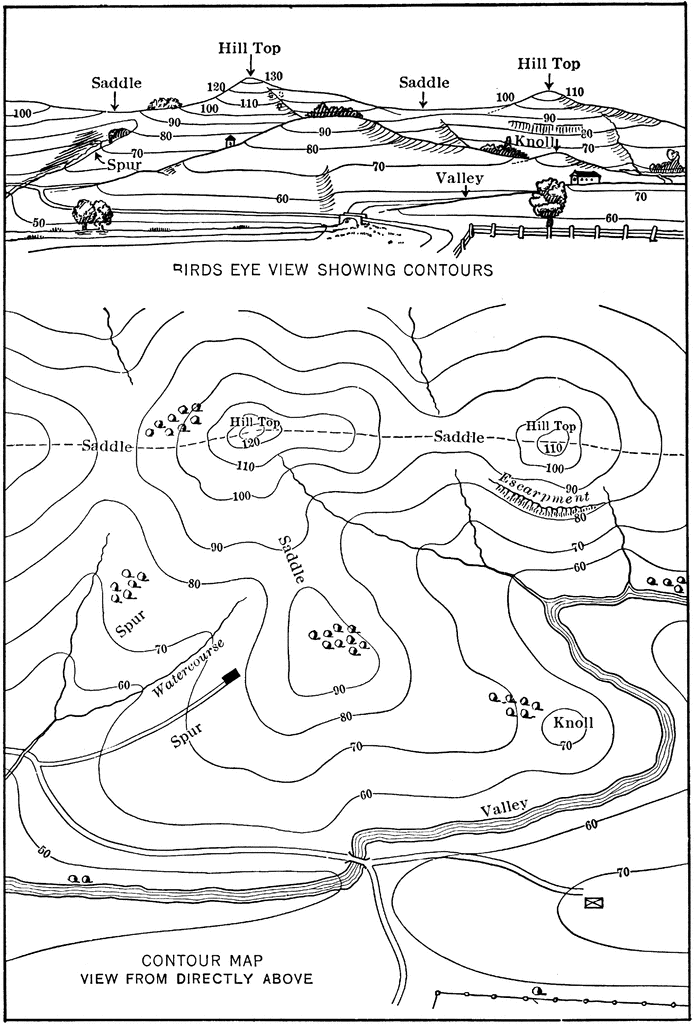
\includegraphics[width=.5\textwidth]{images/contour-map.png}\label{img:fcit-contour-diagram}
\hfill  
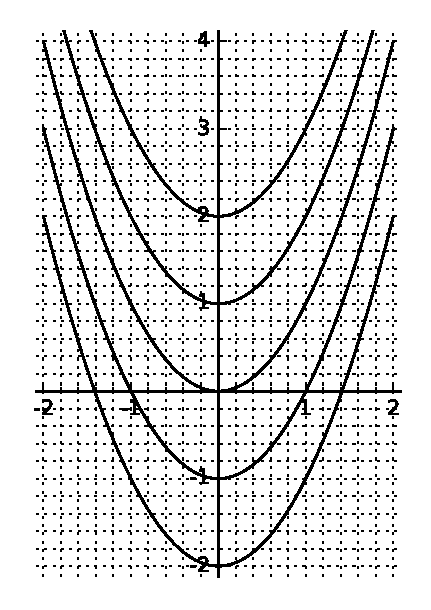
\includegraphics[width=.48\textwidth]{images/parabolas.eps}\label{img:sage-parabolas-gradient}

\begin{ex}
    Let $f(x,y)=y-x^2$. Level curves for $c=-2,-1,0,1,2$ are given above. Determine the direction of and sketch the gradient vector $\nabla f(a,b)$ at the following points: $(0,2)$, $(1,-1)$, $(-1,2)$.
    \vfill\mbox{}
    \let\thefootnote\relax\footnote{Clipart courtesy FCIT, \href{https://etc.usf.edu/clipart/}{\tt https://etc.usf.edu/clipart/}.}
    \addtocounter{footnote}{-1}\let\thefootnote\svthefootnote

\end{ex}

\pagebreak 



\newlecture

\setcounter{section}{6}
%\def\textbookchapter{Chapter 10: Derivatives of Multivariable Functions}
\def\coursetopicnumber{II}
\def\topic{Optimization} % this is the printed title
\def\shorttopic{Optimization} % short topic
\def\textbookname{Active Calculus} % this is the corresponding textbook
\def\shorttextbookname{AC} % this is the short name for the book
\def\textbooksection{10.7} % corresponding textbook section
\def\textbooksectionurl{https://activecalculus.org/vector/S-10-7-Optimization.html} % URL for textbook section
\def\handoutday{} % this is the printed date

\thispagestyle{plain}
\topstuff

%%%%%%%%% DOCUMENT CONTENT STARTS BELOW

\section{\topic{} \booklink{}}
\label{sec:optimization}
\subsection{Optimization with single-variable functions}

Our goal here is to compute local maxima/minima of functions. We begin with single-variable functions. We'll assume these functions are continuous on their domains.

\begin{defn}[Critical points]
    A function $f(x)$ has a \emph{critical point} at $x=a$ if $f'(a)=0$ or if $f'(a)$ does not exist.
\end{defn}%\vspace{.6in}

\begin{prop}
    If $f(x)$ has a local extremum (i.e., a minimum or a maximum) at $x=a$, then $x=a$ is a critical point of $f$.
\end{prop}

Therefore, to find local extrema of a function $f(x)$, we can find the critical points of $f$ and then classify them. Caution: some critical points are neither local minima nor maxima! We call them \emph{terrace points}.

In Calculus I, we saw two methods for classifying critical points: the number line method; and the second derivative test. We'll focus on the latter here.
\begin{prop}[Second Derivative Test for Single-Variable Functions]
    If $f(x)$ has a critical point at $x=a$, then
    \begin{itemize}
        \item if $f''(a)>0$, then %$f(x)$ has a local minimum at $x=a$;
        \bigskip
        \item if $f''(a)<0$, then %$f(x)$ has a local maximum at $x=a$;;
        \bigskip
        \item if $f''(a)=0$, then %this test is inconclusive. ($f(x)$ may have a local minimum, a local maximum, or a terrace point at $x=a$.)
        \bigskip
    \end{itemize}
\end{prop}
\bigskip 

Why?! One way to see why the second derivative test makes sense is to consider the degree-two Taylor polynomial of $f(x)$ at $x=a$ in the case where $f'(a)=0$. When this occurs, the Taylor polynomial is
\begin{align*} 
    T_2(x) 
    &= f(a) + f'(a)\cdot(x-a)+\frac{f''(a)}{2}\cdot(x-a)^2 \\
    & = f(a) + \frac{f''(a)}{2}\cdot(x-a)^2.
\end{align*}
Thus, for $x$-values near $x=a$, 
\[
    f(x)\approx T_2(x)=f(a)+\frac{f''(a)}{2}\cdot(x-a)^2.
\]
If $f''(a)>0$, this is an upward-opening parabola with vertex at $(a,f(a))$. \\ 
If $f''(a)<0$, this is a downward-opening parabola with vertex at $(a,f(a))$.
\pagebreak 

\subsection{Optimization with multivariable functions}
Now we work with multivariable functions. We'll use $f(x,y)$, though the methods generalize for any number of variables. To simplify things, we'll assume our functions are continuous and differentiable where defined.
\begin{defn}[Open interval]
    An \emph{open interval} of radius $r$ centered at a real number $a$ on the real number line is the set of $x$-values that are less than $r$ units away from $a$. 
\end{defn}

\begin{defn}[Open disc]
    An \emph{open disc} of radius $r$ around a point $P=(a,b)$ in the $xy$-plane is the set of points $Q$ that are less than $r$ units away from $P$. Equivalently, it is the set of points $Q=(x,y)$ such that $|\vec{PQ}|<r$.
\end{defn}

\begin{ex}
    Pictures!
\end{ex}

\vspace{1.5in}

\begin{defn}[Local maximum value]
    A function $f(x,y)$ has a \emph{local maximum} (or \emph{relative maximum}) at a point $(x,y)=(a,b)$ if there is some open disc with positive radius $r$ centered at $(a,b)$ such that $f(a,b)\ge f(x,y)$ for all points $(x,y)$ in the disc. The \emph{local maximum value of $f$ at $(a,b)$} is $f(a,b)$.
\end{defn}

\begin{defn}[Local minimum value]
    A function $f(x,y)$ has a \emph{local minimum} (or \emph{relative minimum}) at a point $(x,y)=(a,b)$ if there is some open disc with positive radius $r$ centered at $(a,b)$ such that $f(a,b)\le f(x,y)$ for all points $(x,y)$ in the disc. The \emph{local minimum value of $f$ at $(a,b)$} is $f(a,b)$.
\end{defn}

\noindent As before, local minimum and maximum values are collectively called \emph{local extreme values} or \emph{local extrema}. Standard examples are upward-opening and downward-opening elliptic paraboloids.

\vspace{1in}

For this course, we will focus primarily on finding and classifying local extrema. We'll see some examples where we can classify global extrema as well. As before, we start with critical points.

\begin{defn}[Critical points]
    A differentiable function $f(x,y)$ has a \emph{critical point} at $(x,y)=(a,b)$ if 
    \[
        \nabla f(a,b)=\vec{0}.
    \]
\end{defn}
\noindent In other words, we need both partial derivatives to equal 0.

\pagebreak 

\begin{ex}\label{ex:find-crit-pts-1}
    Find the critical points of $f(x,y)=x^2+2y^2-4x+4y+6$.
\end{ex} 

\vspace{2in}

\begin{ex}\label{ex:find-crit-pts-2}
    Find the critical points of $f(x,y)=xy(x-2)(y+6)$.
\end{ex}

\vfill

\pagebreak 

\begin{prop}
    If $f(x,y)$ has a local extremum at $(x,y)=(a,b)$, then $(a,b)$ is a critical point of $f(x,y)$.
\end{prop}

Therefore, to find local extrema of a function $f(x,y)$, we can find its critical points and then analyze them. Caution: some critical points are neither local minima nor maxima. We call them \emph{saddle points}.
\vspace{1in}

The second derivative test for multivariable functions helps! First, we need a discriminant.
\begin{defn}
    For a function $f(x,y)$, its \emph{discriminant} $D(x,y)$ is defined as \[D(x,y)=f_{xx}(x,y) f_{yy}(x,y) - f_{xy}(x,y)f_{yx}(x,y).\]
\end{defn}

As we have seen, if the second partials of $f$ are continuous, then Clairaut's Theorem says $f_{xy}(x,y)=f_{yx}(x,y)$, so we can write the discriminant as 
\[
    D(x,y)=f_{xx}(x,y)f_{yy}(x,y)-f_{xy}(x,y)^2.
\]
\medskip 

\begin{prop}[Second Derivative Test for Multivariable Functions]
    For a function $f(x,y)$ and its discriminant $D(x,y)$, if $(a,b)$ is a critical point of $f(x,y)$, then:
    \begin{itemize}
        \item If $D(a,b)>0$ and $f_{xx}(a,b)>0$, then $f$ has \\ %a local minimum at $(a,b)$.\\
        \item If $D(a,b)>0$ and $f_{xx}(a,b)<0$, then $f$ has \\ %a local maximum at $(a,b)$.\\
        \item If $D(a,b)<0$, then $f$ has \\ %a saddle point at $(a,b)$.\\
        \item If $D(a,b)=0$, then \\ %the test is inconclusive.
    \end{itemize}
\end{prop}

\vfill 

Why?! Suppose $(0,0)$ is a critical point of $f$. Then, for $a=f_{xx}(0,0)/2$, $b=f_{xy}(0,0)$, $c=f_{yy}(0,0)/2$, the quadratic approximation (from Section 10.4) of $f(x,y)$ at $(0,0)$ is \[Q(x,y)=f(0,0)+ax^2+bxy+cy^2.\] The quantity $ax^2+bxy+cy^2$ is called a \emph{binary quadratic form}. An analysis into what it looks like -- always $\ge0$, always $\le0$, or neither? -- leads to the conditions above.

\pagebreak 

\begin{defn}
    Given a function $f(x,y)$, the \emph{Hessian matrix} is the $2\times2$ matrix \[\begin{pmatrix}f_{xx}(x,y) & f_{xy}(x,y) \\ f_{yx}(x,y)&f_{yy}(x,y)\end{pmatrix}.\]
\end{defn}

Then $D(x,y)$, the discriminant of $f(x,y)$, is the determinant of the Hessian matrix of $f(x,y)$.

\begin{ex}
    For $f(x,y)=x^2+2y^2-4x+4y+6$, we found in Exercise~\ref{ex:find-crit-pts-1} that $f$ has one critical point at $(x,y)=(2,-1)$. Use the second derivative test to classify it.
\end{ex}

\vfill

\begin{ex}
    For $f(x,y)=xy(x-2)(y+6)$, we found in Exercise \ref{ex:find-crit-pts-2} that $f$ has five critical points. Two of them are $(1,-3)$ and $(2,0)$. Classify them.
\end{ex}

\vfill\vfill

Note: In Section \ref{sec:linearization}, Exercise \ref{ex:first-quadratic-approx}, we found the quadratic approximation of $f(x,y)=xy(x-2)(y+6)$ at $(x,y)=(1,-3)$ is $Q(x,y)=9-9(x-1)^2-(y+3)^2$. Can you see why $Q(x,y)$ has a maximum at $(x,y)=(1,-3)$?

\pagebreak 

\subsection{Applications}
For applications, typically we want to minimize or maximize some sort of quantity, and there may be certain constraints that we need to consider. The following exercises outline the general process.
\begin{ex}
    A shipping company handles rectangular boxes provided the sum of the length, width, and height of the box does not exceed 96 inches. Find the dimensions of the box that meets this condition with the largest volume.
\end{ex}
\pagebreak 
\begin{ex}
    Find the point(s) on the plane $x+2y+3z=6$ closest to the point $(x,y,z)=(1,0,0)$.
\end{ex}

\vfill 
For more examples, see \href{https://activecalculus.org/vector/S-10-7-Optimization.html}{Section 10.7 in our textbook} and/or \href{https://tutorial.math.lamar.edu/Classes/CalcIII/RelativeExtrema.aspx}{Paul's Notes}.


\newlecture
\setcounter{chapter}{11}
\setcounter{section}{0}

\def\textbookchapter{Course Topic III: Multiple Integration}

%\def\textbookchapter{Chapter 11: Multiple Integrals}
\def\coursetopicnumber{III}
\def\topic{Double Riemann Sums and Double Integrals over Rectangles} % this is the printed title
\def\shorttopic{Double Riemann sums, integrals} % short topic
\def\textbookname{Active Calculus} % this is the corresponding textbook
\def\shorttextbookname{AC} % this is the short name for the book
\def\textbooksection{11.1} % corresponding textbook section
\def\textbooksectionurl{https://activecalculus.org/vector/S-11-1-Double-Integrals-Rectangles.html} % URL for textbook section
\def\handoutday{} % this is the printed date

\addtocontents{toc}{\bigskip \large \textbookchapter \normalsize \medskip \par} %% for table of contents
%%%%%%%%% DOCUMENT CONTENT STARTS BELOW

\thispagestyle{plain}
\topstuff
\section{\topic{} \booklink{}}
\label{sec:double-integral-rectangle}

\subsection{Integration in Calculus II}
The main result we need in this section is that the area of an $l\times w$ rectangle is %$l\cdot w$.
\bigskip 

\noindent In Calculus II, we saw the definite integral of a single-variable continuous function $f(x)$ on the interval $[a,b]$:
\[
    \int\limits_a^b f(x)\dx\hspace{3in}\mbox{}
\] 
%\vspace{.2in}

\noindent
\begin{minipage}{.5\textwidth}
    This gives us the signed area under the graph of $y=f(x)$ from $x=a$ to $x=b$. Here's how we evaluate it:
    \begin{itemize}
        \item Chop the interval $[a,b]$ up into $n$ subintervals $I_1, I_2, \dots, I_n$, each of width $\Delta x$ where
        
        \medskip 
        {\centering 
            $\Delta x=\phantom{\frac{b-a}{n}}$
        \par}%\hide{\frac{b-a}{n}}$
        
        \medskip 
        \item Pick a sample point in each subinterval. Call the sample points $x_1^*,\, x_2^*,\, \dots,\, x_n^*$.
        \item Draw rectangles in each subinterval with heights $f(x_1^*),\, f(x_2^*),\, \dots,\, f(x_n^*)$.
    \end{itemize}
\end{minipage}
\begin{itemize}
    \item Add up the areas of the rectangles. 
    
    \noindent Rectangle area = %\hide{f(x_1)\Delta x + f(x_2)\Delta x + \dots + f(x_n)\Delta x}$
    \vspace{.3in}
    
    \item In summation notation, the rectangle area is 
    % $\sum\limits_{k=1}^n f(x_k)\Delta x$.
    \vspace{.2in}
    
    \item There will probably be some error. If we use more rectangles, which will be narrower, we expect less error.
    \item If we let $n\to\infty$, the error will go to 0. In this case, the signed area under the graph of $y=f(x)$ from $x=a$ to $x=b$ is 
    %\[\lim\limits_{n\to\infty}\left(\sum\limits_{i=1}^n f(x_i^*)\Delta x\right)=\int\limits_a^b f(x)\dx.\]
\end{itemize}
%\end{minipage}
\vfill 

\pagebreak 

\subsection{Integration in Calculus III}
The main result we need now is that the volume of an $l\times w\times h$ rectangular box is % $l\cdot w\cdot h$.
\bigskip 

Now we think about a continuous function $f(x,y)$ and its graph $z=f(x,y)$ over a domain $R$ that is a rectangle in the $xy$-plane. This is a surface in $\mathbb{R}^3$. We'll be interested in the signed volume of the solid region under the graph of $z=f(x,y)$.

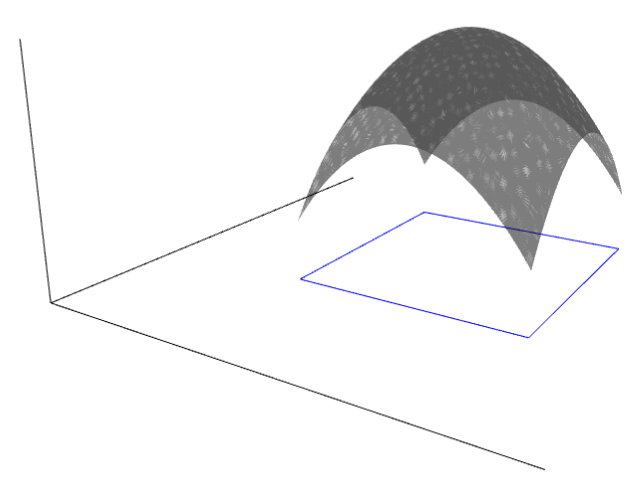
\includegraphics[width=.4\textwidth]{images/mesh1.png}\label{img:sage-double-int-1}

\begin{minipage}{.55\textwidth}
    For now, we'll focus on the rectangular region $[a,b]\times[c,d]$ in the $xy$-plane. In other words, points $(x,y)$ with $a\le x\le b$ and $c\le y\le d$ in the $xy$-plane. Just as we chopped up an interval into subintervals in Calculus I, we'll chop this rectangle up into subrectangles. Here's how we evaluate the signed volume.
    
    \begin{itemize}
        \item Chop the interval $[a,b]$ of $x$ values into $m$ intervals of width $\Delta x$. Thus 
        \[\Delta x = \hspace{1.5in} \] 
        %\frac{b-a}{m}$.
        %\medskip 
        
        \item Chop the interval $[c,d]$ of $y$ values into $n$ intervals of width $\Delta y$. Thus
        \[
            \Delta y = \hspace{1.5in} 
            \]
        %\frac{d-c}{n}$.
        %\medskip 
        
        \item Now we have $mn$ subrectangles which we list with double indices: 
        \[
            \left\{
                \begin{array}{cccc}
                    R_{1,1}, & R_{1,2}, & \dots, & R_{1,n}, \\
                    R_{2,1}, & R_{2,2}, & \dots, & R_{2,n}, \\
                    \vdots & \vdots & \ddots & \vdots \\
                    R_{m,1}, & R_{m,2}, & \dots, & R_{m,n}
                \end{array}
            \right.
        \]
        
        \item Each subrectangle has area $\Delta A = $%\Delta x \Delta y$.
        \item In each subrectangle $R_{i,j}$, pick a sample point $P_{i,j}=(x_{i,j}^*,y_{i,j}^*)$.
    \end{itemize}
\end{minipage}

\pagebreak 

\begin{itemize}
    \item Draw a rectangular box in each subrectangle $R_{i,j}$ with height $f(P_{i,j})$.
    \medskip 

    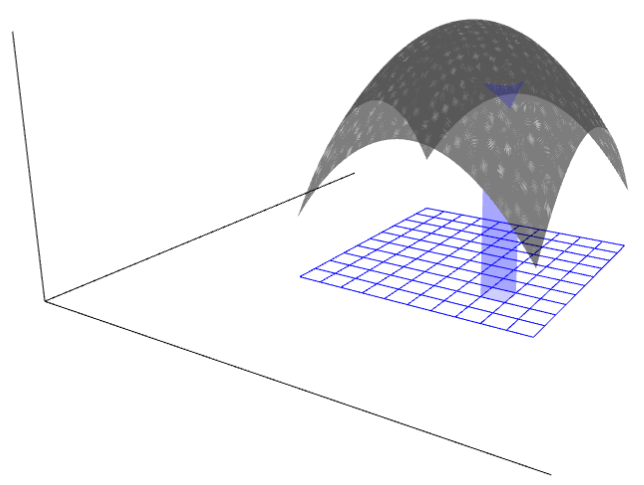
\includegraphics[width=.45\textwidth]{images/mesh2.png}\label{img:sage-double-int-2}
    \medskip 

    %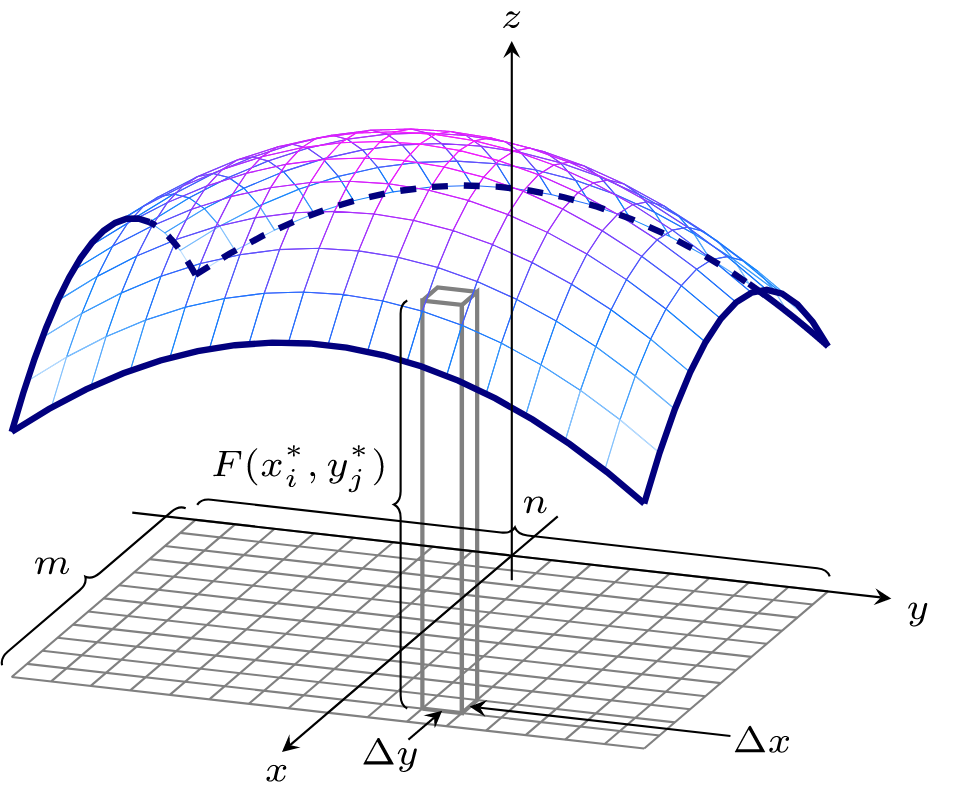
\includegraphics[width=.7\textwidth]{images/riemann2.png}\\
    \item The volume of the rectangular box above rectangle $R_{i,j}$ is % $f(P_{i,j})\delta A = f(x_i,y_j)\Delta A$.
    \item Add up the volumes of the rectangular boxes. \medskip 
    
    Rectangular box volume = $\left\{\begin{array}{cccc}
    f(P_{1,1})\Delta A &+ f(P_{1,2})\Delta A &+ \dots &+ f(P_{1,n})\Delta A \\ 
    +f(P_{2,1})\Delta A &+ f(P_{2,2})\Delta A &+ \dots &+ f(P_{2,n})\Delta A \\ 
    \vdots & \vdots & \ddots & \vdots \\ 
    +f(P_{m,1})\Delta A &+ f(P_{m,2})\Delta A &+ \dots &+f(P_{m,n})\Delta A.\end{array}\right.$
    \medskip 
    
    \item In summation notation, the rectangular box volume is
    %\[\sum\limits_{i=1}^m \sum\limits_{j=1}^n f(x_i^*,y_j^*)\Delta A.\]
    \vspace{1in}
    
    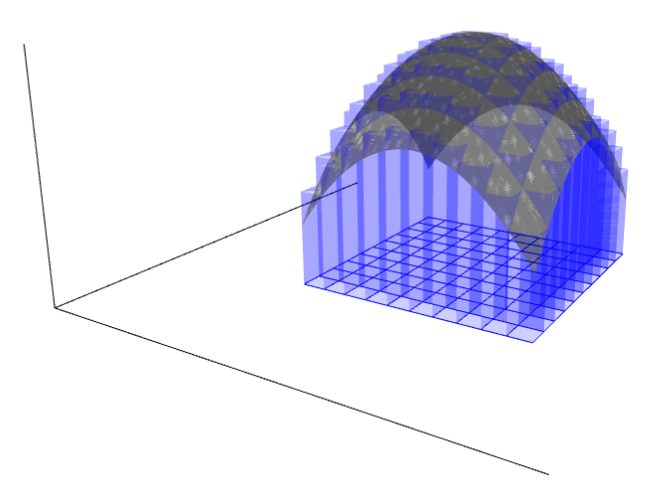
\includegraphics[width=.45\textwidth]{images/mesh3.png}
    \hfill 
    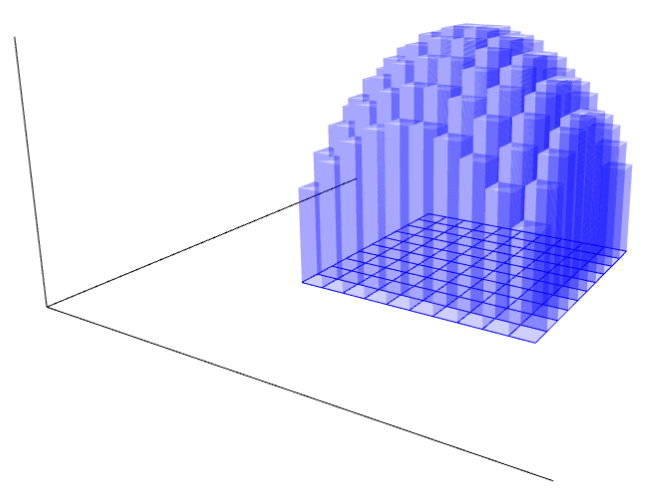
\includegraphics[width=.45\textwidth]{images/mesh4.png}
    
    \item There will probably be some error. If we use more rectangular boxes, which are then narrower in the $x$- and $y$-directions, we'll have less error.
    
    \pagebreak 
    
    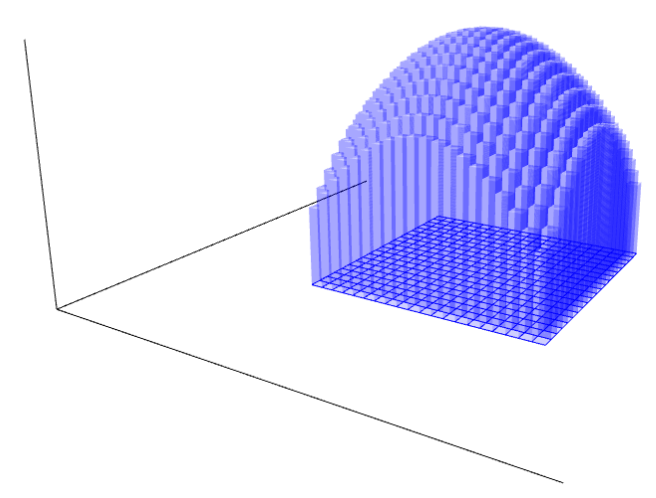
\includegraphics[width=.5\textwidth]{images/mesh5.png}\medskip \label{img:sage-double-int-3}
    
    \item If we let $m\to\infty$ and $n\to\infty$, the error will go to 0. In this case, the signed volume under the graph of $z=f(x,y)$ with $x$ from $a$ to $b$, and with $y$ from $c$ to $d$, is
    \[
        \phantom{\lim\limits_{m\to\infty}\lim\limits_{n\to\infty}\sum\limits_{i=1}^m\sum\limits_{j=1}^nf(x_{i,j}^*,y_{i,j}^*)\Delta A.}
    \]
\end{itemize}

\subsection{Double integral over a rectangle}
\begin{defn}[Double integral]
    In general, if we have a function $f(x,y)$ and want to find the (signed) volume under the graph of $z=f(x,y)$ over a rectangular region $R$ in the $xy$-plane, we write this as 
    \[
        \lim\limits_{m\to\infty}\lim\limits_{n\to\infty}\sum\limits_{i=1}^m\sum\limits_{j=1}^nf(x_{i,j}^*,y_{i,j}^*)\Delta A=\phantom{\iint\limits_R f(x,y)\dA.}
    \] 
    We call this the \emph{double integral of $f$ over $R$}.
\end{defn}

In Section \ref{sec:iterated-integration}, we will see how to evaluate a double integral over a rectangle $R$. In Sections \ref{sec:double-int-general-region} and \ref{sec:double-int-polar}, we will see how to evaluate double integrals over more general regions.
\bigskip 

\subsection{A first example}
We can occasionally use geometry to evaluate a double integral.

\begin{ex}\label{ex:double-integral-via-geometry}
    Let $f(x,y)=5$. For $R=[0,2]\times[1,4]$, evaluate $\iint\limits_R f\dA$.
\end{ex}

\vfill 

\pagebreak 

\subsection{Approximations}
In Calculus I/II, we primarily dealt with integrals in two ways: computing approximations via Riemann sums; and finding exact values via the Fundamental Theorem of Calculus.

In this course we will primarily focus on cases where we can obtain exact solutions for double integrals. Our primary tool is that of the \emph{iterated integral} which allows us to write a double integral as a combination of two single integrals, which we can then evaluate using methods from Calculus II. 

However, there may be times where we cannot get an exact value. When that occurs, approximation techniques like those from Calculus II can be used effectively. Here's an example.
\begin{ex}
    For the rectangle $R=[0,4]\times[-1,5]$, approximate the double integral $\iint\limits_R x^2y\dA$. Do so by subdividing $[0,4]$ up into $m=2$ subintervals, subdividing $[-1,5]$ into $n=3$ subintervals, and choosing sample points to be the midpoint of each rectangle.
\end{ex}


\newlecture
\setcounter{chapter}{11}
\setcounter{section}{1}

%\def\textbookchapter{Chapter 11: Multiple Integrals}
\def\coursetopicnumber{III}
\def\topic{Double Riemann Sums and Double Integrals over Rectangles} % this is the printed title
\def\shorttopic{Iterated integrals} % short topic
\def\textbookname{Active Calculus} % this is the corresponding textbook
\def\shorttextbookname{AC} % this is the short name for the book
\def\textbooksection{11.2} % corresponding textbook section
\def\textbooksectionurl{https://activecalculus.org/vector/S-11-2-Iterated-Integrals.html} % URL for textbook section
\def\handoutday{} % this is the printed date

%%%%%%%%% DOCUMENT CONTENT STARTS BELOW

\thispagestyle{plain}
\topstuff
\section{\topic{} \booklink{}}
\label{sec:iterated-integration}
We can use techniques from Calculus II to evaluate $\iint\limits_R f\dA$, the double integral of $f(x,y)$ over the rectangle $R=[a,b]\times[c,d]$. Earlier, we imagined chopping $R$ up into subrectangles, selecting a sample point in each subrectangle. To simplify things slightly, we can imagine choosing sample $x$-values $x_1^*, x_2^*, \dots, x_m^*$ in $[a,b]$ and sample $y$-values $y_1^*, y_2^*, \dots, y_n^*$ in $[c,d]$, combining them to choose the sample point $(x_i^*,y_j^*)$ in the rectangle $R_{i,j}$.

Since $\Delta A=\Delta x \Delta y$, we have 
\[
    \iint\limits_R f(x,y)\dA = \lim\limits_{m\to\infty}\lim\limits_{n\to\infty}\sum\limits_{i=1}^m\sum\limits_{j=1}^nf(x_i^*,y_j^*)\Delta x\Delta y\hspace{2in}\mbox{}
\]

\vfill
\begin{thm}[Fubini's Theorem]
    Let $f$ be continuous on the rectangular region $R=[a,b]\times[c,d]$. The double integral of $f$ over $R$ is equal to both of the following iterated integrals:
    \[
        \iint\limits_R f(x,y)\dA = \int\limits_{y=c}^{y=d}\, \int\limits_{x=a}^{x=b} f(x,y)\dx\dy = \int\limits_{x=a}^{x=b}\,\int\limits_{y=c}^{y=d} f(x,y)\dy\dx.
    \]
\end{thm}
\bigskip 

In Chapter 10, we learned about partial derivatives. To take a partial derivative of a function (like $f(x,y)$), we need to know which variable we are differentiating with respect to (which is determined by the partial derivative operator, like $\frac{\partial}{\partial x}$), and we treat any other variables as constants. 

The same process applies with integration. If we are integrating a function (like $f(x,y)$), we need to know which variable we are integrating with respect to (which is determined by the differential, like $\dx$), and we treat any other variables as constants.

\pagebreak 

\subsection{The iterated integral process}
To evaluate an iterated integral, we first evaluate the inner integral, then we plug the result of that into the outer integral, and then evaluate the outer integral.

\begin{ex}
    In Exercise~\ref{ex:double-integral-via-geometry} from Section 11.1, we used geometry to evaluate $\iint\limits_R f\dA$ for $f(x,y)=5$ and $R=[0,2]\times[1,4]$. Evaluate this integral as an iterated integral.
\end{ex}

\vfill 

\begin{ex}
    Draw the rectangle $R$ given by $[0,1]\times[2,4]$. Then evaluate the double integral of $f(x,y)=6-2x-y$ over $R$. Do so for both possible variable orders.
\end{ex}

\vfill \vfill 

\pagebreak 

\begin{ex}
    Let $f(x,y)=ye^{xy}$. Let $R$ be the rectangle given by $0\le x\le 1$ and $0\le y\le\ln2$. Find the volume of the solid that lies under the graph of $z=f(x,y)$ and above the rectangle $R$. %Evaluate $\displaystyle\iint\limits_R f(x,y)\dA$.
\end{ex}

\newlecture
\setcounter{chapter}{11}
\setcounter{section}{2}

%\def\textbookchapter{Chapter 11: Multiple Integrals}
\def\coursetopicnumber{III}
\def\topic{Double Integrals over General Regions} % this is the printed title
\def\shorttopic{Double integrals, general regions} % short topic
\def\textbookname{Active Calculus} % this is the corresponding textbook
\def\shorttextbookname{AC} % this is the short name for the book
\def\textbooksection{11.3} % corresponding textbook section
\def\textbooksectionurl{https://activecalculus.org/vector/S-11-3-Double-Integrals-General.html} % URL for textbook section
\def\handoutday{} % this is the printed date

%%%%%%%%% DOCUMENT CONTENT STARTS BELOW

\thispagestyle{plain}
\topstuff
\section{\topic{} \booklink{}}
\label{sec:double-int-general-region}

\subsection{Double integrals over rectangles}
The simplest kind of region $R$ in the $xy$-plane is a rectangle. Any rectangle can be described as the set of points $(x,y)$ where 
\[
    a\le x\le b \quad \text{ and } \quad c\le y\le d
\] 
for some constants $a,b,c,d$ with $a\le b$ and $c\le d$. 

In order to compute the double integral of some function $f(x,y)$ over such a rectangle $R$, we use \emph{iterated integrals} as described in Section~\ref{sec:double-integral-rectangle}:
\[
    \iint\limits_R f(x,y)\dA 
    = \int\limits_{y=c}^{y=d} \left(\,\int\limits_{x=a}^{x=b} f(x,y)\dx\right) \dy 
    = \int\limits_{x=a}^{x=b}\left(\,\int\limits_{y=c}^{y=d} f(x,y)\dy\right)\dx.
\] 
This gives us the (signed) volume under the graph of $z=f(x,y)$ over the region $R$.

Often we will get lazy and write this without parentheses and/or without equal signs in the endpoints of the integral:
\[
    \iint\limits_R f(x,y)\dA 
    = \int\limits_{c}^{d} \int\limits_{a}^{b} f(x,y)\dx \dy 
    = \int\limits_{a}^{b} \int\limits_{c}^{d} f(x,y)\dy \dx .
\] 
\textbf{Note that the order of the differentials matters. It lets us know which variables our endpoints represent.}

\subsection{Descriptions of general regions}
Before we can think about double integrals over general regions, we need to see how to describe general regions with inequalities.

\begin{center}
    \textbf{The key to doing this well is sketching graphs and labeling functions \\ and intersection points.}
\end{center} 
This process is similar to those of computing areas of regions between curves and computing volumes of solids of revolution in Calculus II.

Our typical approach to describe a region $R$ is to describe it as the set of points $(x,y)$ that satisfy inequalities in one of the following ways:
\[
    a\le x\le b\quad \text{ and } \quad g(x)\le y\le h(x)\hspace{2in}\mbox{}
\] 
\[
    \text{ or }\hspace{2in}\mbox{}
\] 
\[
    c\le y\le d \quad \text{ and } \quad g(y)\le x\le h(y)\hspace{2in}\mbox{}
\]
\pagebreak 

\begin{ex}
    Draw the region $R$ described by $-1\le x\le 2$ and $x^2\le y\le 5$.
\end{ex}

\vfill

\begin{ex}
    Draw the region $R$ described by $0\le y\le 6$ and $-y/2\le x\le y/2$.
\end{ex} 

\vfill 

\pagebreak 

\begin{ex}\label{ex:region-inequalities}
    In the $xy$-plane, consider the triangle $T$ that has vertices $(2,0)$, $(6,0)$, and $(6,8)$. Represent this triangle with inequalities in both ways.
\end{ex}

\vfill

\begin{ex}
    Using inequalities, describe the region $R$ in the $xy$-plane bounded by the graphs of $y=4x$ and $y=x^2$.  %Do this both ways (using bottom and top functions; and using left and right functions).
\end{ex}

\vfill



\pagebreak 
\begin{ex}
    Draw the region $R$ in the $xy$-plane bounded by the graphs of $y=2x$, $y=6-x$, and the $y$-axis. Label each curve and intersection points. Then describe it with inequalities.
\end{ex}

\vfill 

\begin{ex}
    Draw the region $R$ in the $xy$-plane bounded by the graphs of $y=2x$, $y=6-x$, and $y=1$. Label each curve and intersection points. Then describe it with inequalities.
\end{ex}

\vfill 

\pagebreak 

\subsection{Integrating over general regions via iterated integrals}
Once we have described a region $R$ with inequalities, we can compute a double integral of a function $f(x,y)$ over $R$ via iterated integrals. This allows us to compute the (signed) volume of 3D region below the surface $z=f(x,y)$ and above the region $R$.
\begin{itemize}
    \item If $R$ is described by $a\le x\le b$ and $g(x)\le y\le h(x)$, then \[\iint\limits_R f(x,y)\dA = \int\limits_{x=a}^{x=b} \left(\,\int\limits_{y=g(x)}^{y=h(x)}f(x,y)\dy\right)\dx.\]
    More simply, 
    \[
        \iint\limits_R f(x,y)\dA = \hspace{2in}
    \]
    %\int\limits_a^b\int\limits_{g(x)}^{h(x)}f(x,y)\dy \dx.\]
    \item If $R$ is described by $c\le y\le d$ and $g(y)\le x\le h(y)$, then 
    \[
        \iint\limits_R f(x,y)\dA = \int\limits_{y=c}^{y=d} \left(\,\int\limits_{x=g(y)}^{x=h(y)}f(x,y)\dx\right)\dy.
    \]
    More simply, 
    \[
        \iint\limits_R f(x,y)\dA = \hspace{2in}
    \]
    %\int\limits_c^d\int\limits_{g(y)}^{h(y)}f(x,y)\dx \dy.\]
\end{itemize}
We then proceed as we did before with iterated integrals, evaluating the inner integral first, and then evaluating that in the outer integral.

\begin{example}
    In Exercise~\ref{ex:region-inequalities}, we described the triangle $T$ with the inequalities in two ways.
    Our first description of $T$ was
    \begin{center}
        $2\le x\le 6$ \quad and \quad  $0\le y\le 2x-4$.
    \end{center}
    Thus, for any function $f(x,y)$, the double integral of $f$ over $T$ is
    \[\iint\limits_T f\dA = \phantom{\int\limits_2^6 \int\limits_0^{2x-4} f(x,y)\dy\dx.}\]
    Our second description of $T$ was
    \begin{center}
        $0\le y\le 8$ \quad and \quad $(y+4)/2\le x\le 6$.
    \end{center}
    Thus, for any function $f(x,y)$, the double integral of $f$ over $T$ is 
    \[\iint\limits_T f\dA = \phantom{\int\limits_0^8 \int\limits_{(y+4)/2}^6 f(x,y)\dx\dy.}\]
    
    This provides flexibility, as the inner integral may be easier to integrate in terms of one variable than it is in terms of the other.
\end{example}
\pagebreak 
\begin{ex}
    Evaluate the iterated integral $\displaystyle\int\limits_{-2}^0\int\limits_{0}^{\sqrt{4-x^2}} y\dy \dx$. Also, draw the region $R$ that this double integral is over.
\end{ex}
\vfill 

\begin{ex}
    Evaluate the following double integral (perhaps changing the limits of integration).
    \[
        \int\limits_0^2\int\limits_y^2 \ee^{x^2}\dx\dy
    \]
\end{ex}


\vfill

\newlecture
\setcounter{chapter}{11}
\setcounter{section}{4}

%\def\textbookchapter{Chapter 11: Multiple Integrals}
\def\coursetopicnumber{III}
\def\topic{Double Integrals in Polar Coordinates} % this is the printed title
\def\shorttopic{Double integrals, polar coordinates} % short topic
\def\textbookname{Active Calculus} % this is the corresponding textbook
\def\shorttextbookname{AC} % this is the short name for the book
\def\textbooksection{11.5} % corresponding textbook section
\def\textbooksectionurl{https://activecalculus.org/vector/S-11-5-Double-Integrals-Polar.html} % URL for textbook section
\def\handoutday{} % this is the printed date

%%%%%%%%% DOCUMENT CONTENT STARTS BELOW

\thispagestyle{plain}
\topstuff
(We are covering Section 11.5, which is on double integrals in polar coordinates, before we cover Section 11.4, which is on applications of double integrals.)
\section{\topic{} \booklink{}}
\label{sec:double-int-polar}
\subsection{Polar coordinates}
Our usual way of representing a point $P$ in the $xy$-plane is with \emph{Cartesian} (or \emph{rectangular}) coordinates $x$ and $y$. For instance, if $P=(5,2)$, then the origin and $P$ are opposite corners on a $5\times2$ rectangle with edges along the $x$- and $y$-axes.
\vspace{1.5in}

We can use circles in place of rectangles. This leads to \emph{polar} coordinates $r$ and $\theta$. Any point $P$ lies on a circle of radius $r\ge0$ centered at the origin at an angle $\theta$ above the positive $x$-axis.

\vfill

\begin{ex}
    Convert $(r,\theta)=(7,\pi/3)$ to rectangular coordinates $(x,y)$. Then convert $(x,y)=(-4,0)$ to polar coordinates $(r,\theta)$.
\end{ex}

\vspace{1in}

\pagebreak 

\subsection{Describing regions with polar coordinates}
\begin{ex}
    Draw the region $R$ of points $P$ that have $1\le r\le 2$ and $\pi/4\le\theta\le \pi$.
\end{ex}

\vspace{1.5in}

\begin{ex}
    Use polar coordinates to describe the region between circles of radii 3 and 5 centered at the origin.
\end{ex}

\vspace{2in}

%\subsection{Double integration over a polar region}
\subsection{Area of a subrectangle in rectangular coordinates}
Suppose you're at the point $P=(x,y)$. Draw a rectangle of width $\Delta x$ and height $\Delta y$ at $P$. The area of the rectangle is 
\[
    \Delta A = \hspace{7in} 
\]

\vfill 
Thus, with rectangular coordinates, the double integral of a function $f$ over a region $R$ is \bigskip 

\[
    \iint\limits_R f \dA = \hspace{3in} 
\]

\vspace{1in}

\pagebreak 

\subsection{Area of a ``subrectangle'' in polar coordinates}
Suppose you're at the point $P=(r,\theta)$. Draw a polar ``rectangle'' with angle $\Delta \theta$ and radius $\Delta r$. Its area is \[\Delta A = \hspace{7in}\]
\vspace{2in}

Thus, with polar coordinates, the double integral of a function $f$ over a region $R$ is \bigskip 

\[
    \iint \limits_R f \dA = \hspace{3in} 
\]

\medskip 

\subsection{Evaluating double integrals using polar coordinates}
\begin{framed}
    \noindent 
    To evaluate a double integral of a function $f$ over a region $R$, the choice of coordinates (rectangular or polar) depends entirely on the region $R$. It does not depend on the function $f$.
\end{framed}
\bigskip 

Essentially, if $R$ can be easily described using polar coordinates, which typically occurs when $R$ contains all of or a portion of a disc, we will do the following: 
\begin{itemize} 
    \item describe $R$ with inequalities for $r$ and $\theta$; 
    \item write $f$ using polar coordinates (using $x=r\cos\theta$, $y=r\sin\theta$); 
    \item write $\dA=r \dr \dtheta$ (or $\dA=r \dtheta \dr$); and 
    \item take the iterated integral approach, using the bounds from the inequalities for $r$ and $\theta$ as the iterated integral endpoints, matching the order of the inner and outer integrals with the order of $\dr$ and $\dtheta$.
\end{itemize} 
\pagebreak 

\begin{ex}
    Let $R$ be the top left quarter of a disc of radius 2 centered at the origin. Describe $R$ with rectangular coordinates and with polar coordinates. Then, for $f(x,y)=3x+1$, evaluate $\iint\limits_R f\dA$ using either rectangular or polar coordinates. 
\end{ex}
\vfill

\begin{ex}
    Find the volume of the solid bounded by the paraboloid $z=9-x^2-y^2$ and the $xy$-plane.
\end{ex}
\vfill 

\pagebreak

\begin{ex}
    Evaluate the following iterated integral by first converting it to polar coordinates:
    \medskip 
    
    \noindent $\displaystyle \int\limits_0^{\sqrt{2}/2} \int\limits_x^{\sqrt{1-x^2}} 4xy\dy\dx$
\end{ex}
\vfill 

\begin{ex}
    Evaluate $\displaystyle\int\limits_0^6 \int\limits_{-\sqrt{36-x^2}}^{\sqrt{36-x^2}} \ee^{-3x^2-3y^2}\dy\dx$.
\end{ex}
\vfill 

%\begin{ex}
%    Find the volume of the region beneath the surface $z=xy+10$ and above the annular region $R$ described with polar coordinate inequalities by $R=\{(r,\theta) : 2\le r\le 4,\, 0\le \theta\le 2\pi\}$.
%\end{ex}

\newlecture
\setcounter{chapter}{11}
\setcounter{section}{3}


%\def\textbookchapter{Chapter 11: Multiple Integrals}
\def\coursetopicnumber{III}
\def\topic{Applications of Double Integrals} % this is the printed title
\def\shorttopic{Applications of double integrals} % short topic
\def\textbookname{Active Calculus} % this is the corresponding textbook
\def\shorttextbookname{AC} % this is the short name for the book
\def\textbooksection{11.4} % corresponding textbook section
\def\textbooksectionurl{https://activecalculus.org/vector/S-11-4-Double-Integrals-Applications.html} % URL for textbook section
\def\handoutday{} % this is the printed date


%%%%%%%%% DOCUMENT CONTENT STARTS BELOW

\thispagestyle{plain}
\topstuff
\section{\topic{} \booklink{}}
\label{sec:double-integral-apps}
In single-variable calculus, we can use definite integrals to compute the average value of a function on an interval, the area of a region between two curves, and the mass of a one-dimensional object given a density function. We'll push these ideas to multivariable functions.

\subsection{Computing the size of the domain}
\subsubsection{Single-variable}
\begin{ex}
    For an interval $[a,b]$, draw and interpret $\displaystyle\int\limits_a^b \dx$.
\end{ex}

\vspace{1in}

\subsubsection{Multivariable}
\begin{ex}
    For a general region $R$, draw and interpret $\displaystyle\iint\limits_R \dA$.
\end{ex}

\vfill 

\begin{ex}
    Set up an iterated integral to compute the area of the region in the plane enclosed by circles of radius 3 and 4 centered at the origin.
\end{ex}

\vfill

\pagebreak 

\subsection{Average value of a function}
\subsubsection{Single-variable}
The \emph{average value} of a function $f(x)$ on an interval $I=[a,b]$ is
$f_{avg}=\phantom{\displaystyle\dfrac{1}{b-a}\int\limits_a^b f(x)\dx.}$

\vspace{1.5in}

\subsubsection{Multivariable}
The \emph{average value} of a function $f(x,y)$ on a region $R$ is 
$f_{avg}=\phantom{\displaystyle\dfrac{1}{\text{area}(R)}\iint\limits_R f\dA.}$

\vspace{1.5in}

\noindent Note: Since $\text{area}(R)=\displaystyle\iint\limits_R \dA$, we can rewrite the average value of $f$ on $R$ as 
\vspace{.5in}

\begin{ex}
    Set up an iterated integral to compute the average value of the function $f(x,y)=e^{-x^2-y^2}$ over the portion of the disc of radius 3 centered at the origin with $x\ge0$.
\end{ex}

\pagebreak 

\subsection{Domain splitting}
\subsubsection{Single-variable}
Suppose $a<b<c$ and that $f$ is continuous on $[a,c]$. Then $\displaystyle\int\limits_a^c f(x)\dx = \phantom{\int\limits_a^b f(x)\dx + \int\limits_b^c f(x)\dx.}$

\vspace{1in}

\subsubsection{Multivariable}
Suppose $R$ is the union of non-overlapping regions $R_1$ and $R_2$. Then for any function $f$ continuous on $R$, \\ \smallskip 

$\displaystyle\iint\limits_R f\dA = \phantom{\iint\limits_{R_1}f\dA + \iint\limits_{R_2}f\dA.}$

\vspace{1in}

\begin{ex}
    Consider the region $T$ consisting of all points in the triangle formed by the points $(0,0)$, $(6,2)$, and $(3,12)$.  For $f(x,y)=e^{xy}$, write $\displaystyle\iint\limits_T f\dA$ in terms of iterated integrals.
\end{ex}

\pagebreak 

\subsection{Volume of a region between surfaces}
\subsubsection{Single-variable}
If $g(x)\le h(x)$ for all $x$ values in an interval $[a,b]$, then the area of the region enclosed by the graphs of $y=g(x)$ and $y=h(x)$ over $[a,b]$ is \\ 
\smallskip 

\noindent Area = $\phantom{\displaystyle\int\limits_a^b \left(h(x)-g(x)\right)\dx.}$
\vspace{.5in}

\subsubsection{Multivariable}
If $g(x,y)\le h(x,y)$ for all points $(x,y)$ in a region $R$, then the volume of the region enclosed by the graphs of $z=g(x,y)$ and $z=h(x,y)$ over $R$ is \\
\smallskip 

\noindent Volume = $\phantom{\displaystyle\iint\limits_R\left(h(x,y)-g(x,y)\right)\dA}$
\vspace{1in}

Note: If the surfaces $z=g(x,y)$ and $z=h(x,y)$ enclose a region, we will typically need to find the intersection of the surfaces to determine the region $R$. We do this just as we did in the single variable case, equating the two functions and solving, thereby determining the boundary of $R$.
\begin{ex}
    Set up an iterated integral to compute the volume of the region enclosed by the graphs of $z=x^2+y^2$ and $z=2-x^2-y^2$.
\end{ex}

\vfill 

\pagebreak 

\subsection{Mass of an object}
\subsubsection{Single-variable}
Suppose we have an object that lies along the $x$-axis from $x=a$ to $x=b$. Suppose the density of the object is $\delta(x)$ (units of mass / units of $x$) at position $x$. Then the object has\\
\smallskip 

\noindent mass $= \displaystyle\int\limits_a^b \delta(x)\dx$
\vspace{.3in}

\subsubsection{Multivariable}
Suppose we have an object that fills a region $R$ in the $xy$-plane. Suppose the density of the object is $\delta(x,y)$ (units of mass / units of area) at position $(x,y)$. Then the object has \\
\smallskip 

\noindent mass $ = \displaystyle\iint\limits_R \delta(x,y)\dA$

\vspace{.3in}
Units are our guide! We can multiply together the units of the terms in the integral to get the units of the result.
\begin{ex}
    Suppose a flat disc of radius 3 cm has a density of $\frac{1}{1+r}$ grams per cm$^2$ for all points a distance of $r$ cm from the center. Set up an iterated integral to compute the mass of the disc.
\end{ex}
\vfill

\begin{ex}
    Same disc, but suppose the density at the point $(x,y)$ is $(3+x)$ g/cm$^2$. (The disc is centered at the origin.) Set up an iterated integral to compute the mass of the disc. Units?
\end{ex}
\vfill 

\newlecture
\setcounter{chapter}{11}
\setcounter{section}{6}

%\def\textbookchapter{Chapter 11: Multiple Integrals}
\def\coursetopicnumber{III}
\def\topic{Triple Integrals} % this is the printed title
\def\shorttopic{Triple integrals} % short topic
\def\textbookname{Active Calculus} % this is the corresponding textbook
\def\shorttextbookname{AC} % this is the short name for the book
\def\textbooksection{11.7} % corresponding textbook section
\def\textbooksectionurl{https://activecalculus.org/vector/S-11-7-Triple-Integrals.html} % URL for textbook section
\def\handoutday{} % this is the printed date

%%%%%%%%% DOCUMENT CONTENT STARTS BELOW

\thispagestyle{plain}
\topstuff
\section{\topic{} \booklink{}}
\label{sec:triple-integrals}
\subsection{Single, double, triple}
\begin{itemize}
    \item For $f$ a function of one variable and $I$ an interval in the number line, a \emph{single integral} is an integral of the form 
    \[
        \phantom{\int\limits_I f\dx.}
    \]
    $\dx$ is a differential that represents an infinitesimally small unit of length.
    %\vfill 

    \item For $f$ a function of two variables and $R$ a region in the $xy$-plane, a \emph{double integral} is an integral of the form 
    \[
        \phantom{\iint\limits_R f\dA.}
    \]
    $\dA$ is a differential that represents an infinitesimally small unit of area.
    %\vfill\vfill
    
    \item For $f$ a function of three variables and $D$ a region in 3-dimensional space, a \emph{triple integral} is an integral of the form 
    \[
        \phantom{\iiint\limits_D f\dV.}
    \]
    $\dV$ is a differential that represents an infinitesimally small unit of volume.
    %\vfill\vfill
\end{itemize}

In Section \ref{sec:double-integral-apps}, we saw some double integral applications. They also apply to triple integrals.

\begin{itemize}
    \item 
    If $f$ is a function of 3 variables and $D$ is a region in 3-space, then the (signed) volume (?!) of the 4D region below (?!) the graph of $w=f(x,y,z)$ above the region $D$ is
    %\vfill %
    \[
        \phantom{\iiint\limits_D f\dV.}
    \]
    
    \item If an object fills a region $D$ in 3-space, and the density of the object at the point $(x,y,z)$ is $\delta(x,y,z)$ (units of mass per unit of volume), then the total mass of the object is %\vfill
    \[
        \phantom{\iiint\limits_D \delta \dV.}
    \]
    
    \item If $D$ is a region in 3-space, then its volume is 
    %\vfill %
    $\phantom{\displaystyle\iiint \limits_D \dV.}$
    
    \item If $D$ is a region in 3-space, then the average value of a function $f$ on $D$ is 
    %\vfill %
    $\phantom{\displaystyle\dfrac{1}{\text{vol}(D)}\iiint\limits_D f\dV.}$
\end{itemize}

\pagebreak 



\pagebreak 

\subsection{Triple integral, general 3D region, Cartesian coordinates}
Let $D$ be a region in 3-dimensions, and suppose we can describe $D$ by 
\[ 
    a\le x\le b, \quad\quad
    g(x)\le y\le h(x), \quad\quad
    p(x,y) \le z \le q(x,y) 
\]
for constants $a, b$, and functions $g(x)$, $h(x)$, $p(x,y)$, $q(x,y)$.

Then for any function $f$ of $x$, $y$, $z$, we have $\dV=\dz\dy\dx$, so 
\[
    \iiint\limits_D f\dV = 
    \phantom{\int\limits_a^b \int\limits_{g(x)}^{h(x)} \int\limits_{p(x,y)}^{q(x,y)} f(x,y,z)\dz\dy\dx.}
\]

If, instead, we had inequalities with a different order of variables, such as
\[ 
    c\le y\le d, \quad\quad
    g(y)\le z\le h(y), \quad\quad
    p(y,z) \le x \le q(y,z), 
\]
then we would have 
\[
    \iiint\limits_D f\dV = 
    \phantom{\int\limits_c^d \int\limits_{g(y)}^{h(y)} \int\limits_{p(y,z)}^{q(y,z)} f(x,y,z)\dx\dz\dy.}
\]
Of course, there are other possibilities for the inequalities. The differentials must match up with the integral symbols. (Inner, Middle, Outer.) 
\begin{itemize} 
    \item In general, the bounds for Inner can involve variables from %Middle and/or Outer. 
    \\ 
    \item The bounds for Middle can involve the variable from %Outer. 
    \\ 
    \item The bounds for Outer are %constants.
    \\
\end{itemize} 

\noindent 
There are generally two main stages in computing a triple integral:
\begin{enumerate}
    \item \mbox{} \\ 
    \item \mbox{} \\ 
\end{enumerate}

\subsection{Describing 3D regions}
It can be difficult to describe a 3D region! However, we have some tricks. The main idea is to determine bounds for one of the variables (say $z$) in terms of the others (say $x$ and $y$). Then we can project the 3D region into a region in the $xy$-plane. Then we need to describe the region in the $xy$-plane, which we can using either rectangular coordinates (Section \ref{sec:double-integral-rectangle}) or polar coordinates (Section \ref{sec:double-int-polar}).

\pagebreak 

\subsection{Examples}
\begin{ex}
    Set up and evaluate $\displaystyle\iiint\limits_D 6x\dV$ for $D$ the region given by
    \[0\le y\le 1,\quad y\le z\le x,\quad y\le x\le 2y.\]
\end{ex}
\vfill 

\begin{ex}
    Let $W$ be the top half of the unit ball centered at the origin. Describe $W$ with inequalities for $x$, $y$, and $z$. (A \emph{ball} is a filled-in sphere, just as a \emph{disc} is a filled-in circle.) Then, for any function $f$, write down $\iiint\limits_W f\dV$ as an iterated integral.
\end{ex}

\vfill\vspace{1in}

\pagebreak 
\begin{ex}
    How would you determine the average height ($z$-value) of a point in the top half of a ball of radius 3?
\end{ex}

\vspace{1.5in}

\begin{ex}
    A building $B$ has a rectangular base that is 8m wide and 16m long. It has a flat roof that is slanted so that one corner is 12m high and its adjacent corners are 10m high.
    \begin{enumerate}
        \item Describe the building with inequalities for $x$, $y$, $z$.
        \item Set up an iterated integral to compute the building volume.% (which is $\displaystyle\iiint\limits_B \dV$).
        \item Suppose the building is filled with a gas that has density $\delta(x,y,z)=(xy+z)$ kg/m$^3$. Set up an iterated integral to compute the total mass of the gas in the building.
    \end{enumerate}
\end{ex}

\vfill

%\pagebreak 

\pagebreak 

\begin{ex}
    Consider the region $D$ in the first octant under the plane $x+2y+3z=6$. For some function $f(x,y,z)$, write $\displaystyle\iiint\limits_D f\,\dV$ as an iterated integral with differentials in order $\dy \dx \dz$. %Then write it as an iteraged integral with differentials in order $\dy \dx \dz$.
\end{ex}
\vfill


\newlecture
\setcounter{chapter}{11}
\setcounter{section}{7}

%\def\textbookchapter{Chapter 11: Multiple Integrals}
\def\coursetopicnumber{III}
\def\topic{Triple Integrals in Cylindrical and Spherical Coordinates} % this is the printed title
\def\shorttopic{Cylindrical, spherical integration} % short topic
\def\textbookname{Active Calculus} % this is the corresponding textbook
\def\shorttextbookname{AC} % this is the short name for the book
\def\textbooksection{11.8} % corresponding textbook section
\def\textbooksectionurl{https://activecalculus.org/vector/S-11-8-Triple-Integrals-Cylindrical-Spherical.html} % URL for textbook section
\def\handoutday{} % this is the printed date

%%%%%%%%% DOCUMENT CONTENT STARTS BELOW

\thispagestyle{plain}
\topstuff
\section{\topic{} \booklink{}}
\label{sec:triple-spherical-cylindrical}
In Section \ref{sec:double-int-polar}, we saw how to evaluate double integrals using polar coordinates. This choice of coordinates is useful when integrating over a region that has circular symmetry.

When working with triple integrals, we will see two new coordinate systems. Cylindrical coordinates are useful when a region has circular symmetry. Spherical coordinates are useful when a region has spherical symmetry.

\subsection{Cylindrical coordinates}
Cylindrical coordinates are useful for describing a region in $\mathbb{R}^3$ that has some sort of circular symmetry. To describe a point $P$ in $\mathbb{R}^3$, we visualize it as if it is on the rim of a circular cylinder with its base centered at the origin in the $xy$-plane. We describe $P$ with a radius $r$, a height $z$, and an angle $\theta$ on the rim of the face of the cylinder.
\bigskip 

\noindent A point $P=(x,y,z)$ (rectangular coordinates) can be written with \emph{cylindrical coordinates} $(r,\theta,z)$: % as:
\begin{itemize}
    \item $x=\phantom{r\cos(\theta)}$
    \item $y=\phantom{r\sin(\theta)}$
    \item $z=\phantom{z}$
\end{itemize}

\vfill

%We generally take $r\ge0$,\, $0\le \theta<2\pi$,\, and $z\in\mathbb{R}$.
%\subsection{Fundamental surfaces}
%\vspace{2in}


\begin{ex}
    Use cylindrical coordinates to describe a wedge of a cheese wheel of radius 6 cm that is 4 cm tall and has an angle of $30^\circ$.
\end{ex}

\vspace{1.5in}

\pagebreak 

\subsubsection{Differentials for cylindrical coordinates}
To compute  $\iiint\limits_D f\dV$ with cylindrical coordinates, we need $\dV$ in terms of $\dr$, $\dtheta$, $\dz$. \medskip 

\noindent Since cylindrical coordinates are just polar coordinates with $z$, and since $\dV=\dx\dy\dz$, we have \bigskip 

\[
    \dV=\phantom{ \dx\dy\dz=r\dr\dtheta\dz.}\hspace{2in}
\] 

\bigskip 

\begin{framed}
    {\centering 
        \textbf{Method to compute a triple integral using cylindrical coordinates}  
    \par}
    \bigskip 
    
    Given a function $f$ and a region $D$, to compute $\iiint\limits_D f\dV$ using cylindrical coordinates,
    \begin{itemize}
        \item Describe $D$ using inequalities with cylindrical coordinates $r$, $\theta$, $z$.
        \item Put those bounds in as the endpoints of each integral symbol, recalling the order rules.
        \item Write $f$ in terms of cylindrical coordinates (using $x=r\cos\theta$, $y=r\sin\theta$, $z=z$). Keep in mind that $x^2+y^2=r^2$.
        \item Write $\dV = r\dr\dtheta\dz$, with the order of differentials corresponding to the order of the integrals.
        \item Evaluate Inner, then Middle, then Outer. If any integral is difficult, think about putting the differentials in another valid order (if possible).
    \end{itemize} 
\end{framed}

\begin{ex}
    Let $f(x,y,z)=x-2y+z$. Let $D$ be the solid cylinder of radius 3 and height 4 sitting on the $xy$-plane centered on the positive $z$-axis. Write $\displaystyle\iiint\limits_D f\dV$ using cylindrical coordinates.
\end{ex}

\vfill

\pagebreak 
\subsection{Spherical coordinates}
Spherical coordinates are useful for describing a region in $\mathbb{R}^3$ that has some sort of spherical symmetry. To describe a point $P$ in $\mathbb{R}^3$, we think about it as being on a sphere of radius $\rho$ along with two angles: $\theta$ and $\phi$, which are like longitude and latitude.

\subsection{Coordinates}
A point $P=(x,y,z)$ (rectangular coordinates) can be written with \emph{spherical coordinates} $(\rho,\theta,\phi)$:
\begin{itemize}
    \item $x=\phantom{\rho\cos(\theta)\sin(\phi)}$
    \item $y=\phantom{\rho\sin(\theta)\sin(\phi)}$
    \item $z=\phantom{\rho\cos(\phi)}$
\end{itemize}

\vfill 

%We generally take $\rho\ge0$,\, $0\le \theta<2\pi$, and $0 \le \phi \le \pi$.
%\vfill 

%\subsection{Fundamental surfaces}
%\vspace{2in}

\begin{ex}
    Use spherical coordinates to describe the portion of a ball of radius 5 centered at the origin with $y\le0$ and $z\ge0$. %(A \emph{ball} is a filled-in sphere, just as a \emph{disk} is a filled-in circle.)
\end{ex}

\vspace{1.5in}

\pagebreak 

\subsubsection{Differentials for spherical coordinates}
To compute $\displaystyle\iiint\limits_D f\dV$ with spherical coordinates, we need $\dV$ in terms of $\drho$, $\dtheta$, $\dphi$.

If you're at the point $(\rho,\theta,\phi)$ and increase each variable (by $\Delta \rho$, $\Delta \theta$, $\Delta \phi$), the resulting volume is 
\[
    \Delta V \approx \rho^2 \sin\phi \, \Delta \rho\, \Delta \theta \, \Delta \phi.
\]
To understand where this comes from, see \href{https://activecalculus.org/vector/S-11-8-Triple-Integrals-Cylindrical-Spherical.html#A_11_8_8}{Activity 11.8.6 in the textbook}. Thus, for integration purposes, 
\[
    \dV = \phantom{\rho^2\sin\phi \, \drho \dtheta \dphi.}
\]
\bigskip 

(More generally, to understand how differentials work with a change of coordinates for any number of variables, see \href{https://activecalculus.org/vector/S-11-9-Change-of-Variable.html}{Section 11.9 of the textbook, which is titled ``Change of Variables.''})
\begin{framed}
    {\centering 
        \textbf{Method to compute a triple integral using spherical coordinates}  
    \par}
    \bigskip 
    
    Given a function $f$ and a region $D$, to compute $\iiint\limits_D f\dV$ using spherical coordinates,
    \begin{itemize}
        \item Describe $D$ using inequalities with spherical coordinates $\rho$, $\theta$, $\phi$.
        \item Put those bounds in as the endpoints of each integral symbol, recalling the order rules.
        \item Write $f$ in terms of spherical coordinates (using $x=\rho\cos\theta\sin\phi$, $y=\rho\sin\theta\sin\phi$, $z=\rho\cos\phi$). Keep in mind that $x^2+y^2+z^2=\rho^2$.
        \item Write $\dV = \rho^2\sin\phi\drho\dtheta\dphi$, with the order of differentials corresponding to the order of the integrals.
        \item Evaluate Inner, then Middle, then Outer. If any integral is difficult, think about putting the differentials in another valid order (if possible).
    \end{itemize} 
\end{framed}

\begin{ex}
    Let $f(x,y,z)=3+x^2+y^2+z^2$, and let $W$ be the portion of a ball of radius 5 centered at the origin where $y\le0$ and $z\ge0$. Write $\displaystyle\iiint\limits_W f\dV$ as using spherical coordinates.
\end{ex}

\pagebreak 

\subsection{Examples}
Remember, the choice of coordinates depends on the region!
\begin{ex}
    A circular cone $D$ is given by the equation $z=\sqrt{x^2+y^2}$. Suppose a circular cone of height 10 cm is filled with ice cream. The density of the ice cream $z$ cm above the bottom is $(30-z)$g/cm$^3$. Set up a triple integral to compute the mass of the ice cream in the cone using cylindrical coordinates.
\end{ex}

\vfill 

\pagebreak 

\begin{ex}
    Let $D$ be the top half of a ball of radius 7 centered at the origin. Compute the volume of $D$ using a triple integral.
    %Using geometry, determine $\displaystyle\iiint_D\dV$. Write this triple integral as an iterated integral using Cartesian coordinates. Write this triple integral as an iterated integral using spherical coordinates.%Rewrite $\displaystyle\int\limits_{0}^7\int\limits_{-\sqrt{49-z^2}}^{\sqrt{49-z^2}}\int\limits_{-\sqrt{49-y^2-z^2}}^{\sqrt{49-y^2-z^2}}\dx\dy\dz$ as an integral with spherical coordinates. Then evaluate it.%Compute the volume of a sphere of radius 7.
\end{ex}

\vfill

\vspace{.5in}

\pagebreak 

\begin{ex}
    Set up an iterated integral to find the volume of the solid region $D$ which is enclosed by the top half of a unit sphere centered at the origin and a circular cone given by the equation $z=\sqrt{x^2+y^2}$. (If time permits, evaluate it.)
\end{ex}



\newlecture

\setcounter{chapter}{12}
\setcounter{section}{0}

\def\textbookchapter{Course Topic IV: Vector Calculus}
\def\coursetopicnumber{IV}
\def\topic{Vector Fields} % this is the printed title
\def\shorttopic{Vector fields} % short topic
\def\textbookname{Active Calculus} % this is the corresponding textbook
\def\shorttextbookname{AC} % this is the short name for the book
\def\textbooksection{12.1} % corresponding textbook section
\def\textbooksectionurl{https://activecalculus.org/vector/S_Vector_VectorFields.html} % URL for textbook section
\def\handoutday{} % this is the printed date

\addtocontents{toc}{\bigskip \large \textbookchapter \normalsize \medskip \par} %% for table of contents
%%%%%%%%% DOCUMENT CONTENT STARTS BELOW

\thispagestyle{plain}
\topstuff
\section{\topic{} \booklink{}}
\label{sec:vector-fields}
\subsection{Definition and visualization}
Vector fields are ubiquitous in everyday life. We experience them as gravitational fields, electric fields, force fields, fluid flow, wind flow, and so on.

\begin{defn}[Vector Field]
    A \emph{vector field} is a function that takes points as input and gives vectors as output. If the input point is in $\mathbb{R}^n$, then the vector also has $n$ components.
\end{defn}

\begin{example}
    Here are a few examples in 2 and 3 dimensions.
    \begin{multicols}{2}
        \begin{itemize}
            \item $\vec{F}(x,y)=\langle x,\, y\rangle$
            \item $\vec{F}(x,y)=\langle x^2-y^2,\, 0\rangle$
            \item $\vec{F}(x,y,z)=\langle xy,\,  yz,\,  4+x+y\rangle$
            \item $\vec{F}(x,y,z)=\langle 1,\,  2,\,  e^z\rangle$
        \end{itemize}
    \end{multicols}
\end{example}

To visualize a vector field $\vec{F}(x,y)$, do the following:
\begin{itemize}
    \item create a grid of sample points;
    \item at each sample point $P=(x,y)$ (or $P=(x,y,z)$), draw the vector $\vec{F}(P)$ with its tail at $P$.
\end{itemize}

\begin{example}
    Here are a few graphical representations of 2D vector fields.
    \\
    \begin{minipage}{.4\textwidth}
        \begin{center}
            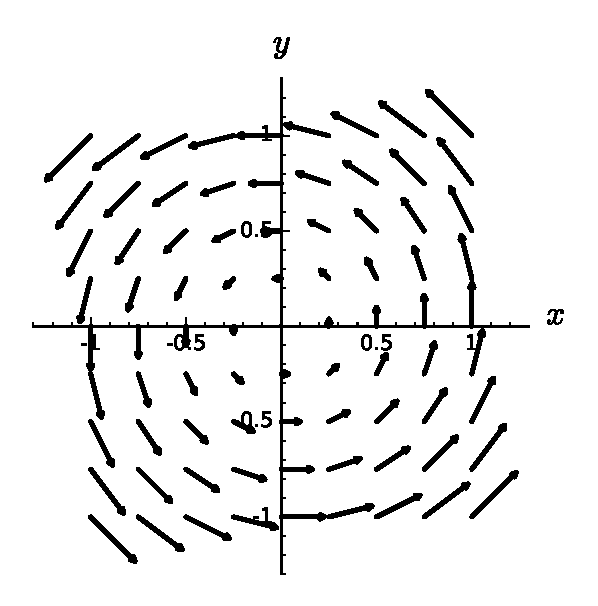
\includegraphics[width=.9\textwidth]{images/vf1.eps}\label{img:sage-vector-field-1} \medskip 
            
            $\vec{F}(x,y) = \left\langle -\dfrac{y}{4}, \, \dfrac{x}{4}\right\rangle$ 
        \end{center}
    \end{minipage}
    \hfill 
    \begin{minipage}{.4\textwidth}
        \begin{center}
            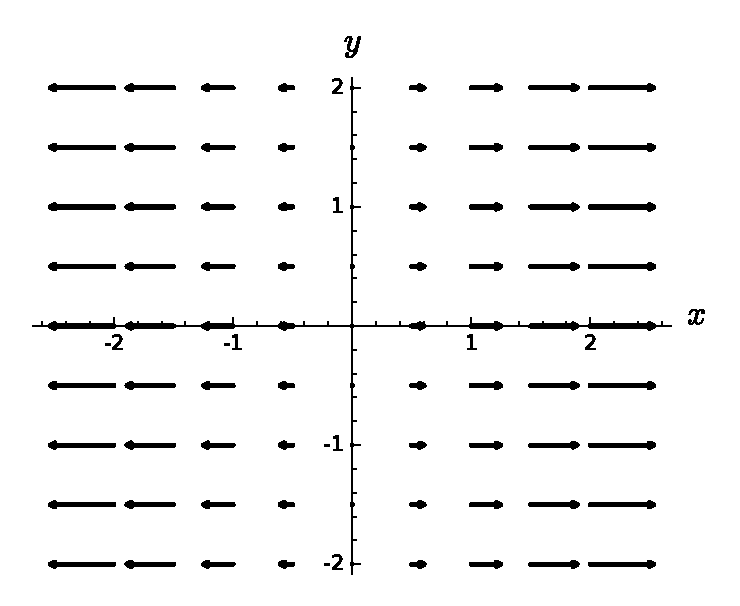
\includegraphics[width=.9\textwidth]{images/vf2.eps} \medskip
            
            $\vec{F}(x,y) = \left\langle \dfrac{x}{3}, \, 0\right\rangle$ 
        \end{center}
    \end{minipage}
\end{example}

We can view a vector field as a velocity field, where each arrow represents a velocity vector (with a direction and a magnitude).

\begin{defn}[Flow curve, stream line]
    A path that follows the directions of a vector field is called a \emph{flow curve} or \emph{stream line}.
\end{defn}
%\pagebreak 

\begin{ex}
    On the axes below, sketch the vector field  $\vec{F}(x,y)=\langle y,\,  -x \rangle$.
    
    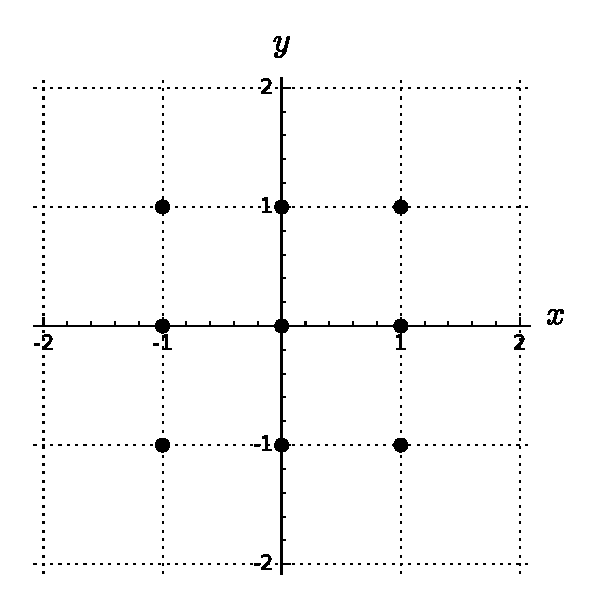
\includegraphics[width=.5\textwidth]{images/dots_fewer}
\end{ex}

\vfill 

\begin{ex}
    On the axes below, sketch the vector field   $\vec{F}(x,y)=\dfrac{1}{2}\vec{i}+\dfrac{x}{2}\vec{j}$.

    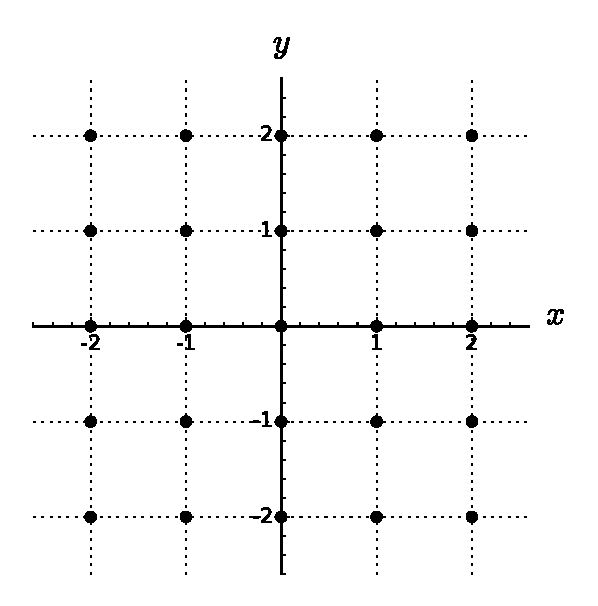
\includegraphics[width=.5\textwidth]{images/dots_more}
\end{ex}

\pagebreak 

\begin{ex}
    Identify the following vector fields with the sketches below. (Some are scaled a bit to avoid overlapping arrows.)
    \begin{multicols}{4}
    \begin{enumerate}
        \item $\vec{F}=\langle 0,\, x^2\rangle$
        \item $\vec{F}=\langle y,\, x\rangle$
        \item $\vec{F}=\langle 2x,\, -y\rangle$
        \item $\vec{F}=\langle x-y,\, x\rangle$
    \end{enumerate}
    \end{multicols}
    
    \begin{minipage}{.4\textwidth}
        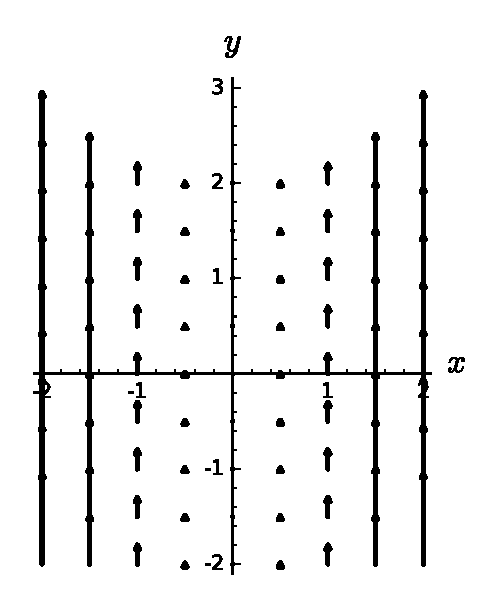
\includegraphics[width=\textwidth]{images/mult1} \label{img:sage-vector-field-2}
    \end{minipage}
    \hfill
    \begin{minipage}{.4\textwidth}
        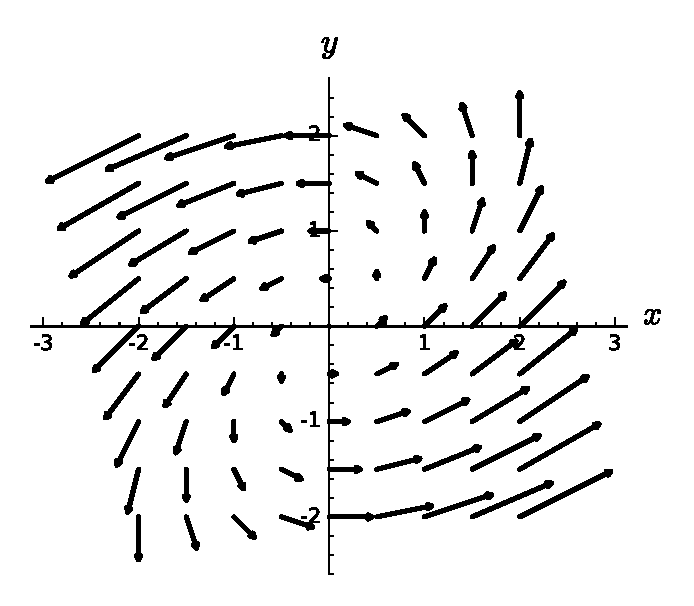
\includegraphics[width=\textwidth]{images/mult2}
    \end{minipage}
    
    \begin{minipage}{.4\textwidth}
        \includegraphics[width=\textwidth]{images/mult3}
    \end{minipage}
    \hfill
    \begin{minipage}{.4\textwidth}
        \includegraphics[width=\textwidth]{images/mult4}
    \end{minipage}
\end{ex}

\subsection{Gradient vector fields}
We learned about the gradient of a multivariable function in Chapter 10. Recall the following.
\begin{defn}[Gradient]
    The \emph{gradient} of a scalar-valued function is a vector-valued function:
    \[
        \nabla f(x,y)=\phantom{\langle f_x(x,y),\, f_y(x,y)\rangle}
    \] 
    and 
    \[
        \nabla f(x,y,z)=\phantom{\langle f_x(x,y,z),\, f_y(x,y,z),\, f_z(x,y,z)\rangle.}
    \]
\end{defn}
\vfill 

\noindent Thus, for any multivariable function $f$ we have a corresponding vector field $\nabla f$.

\pagebreak 

\begin{ex}
    For $f(x,y,z)=xyz$, compute the vector field $\nabla f(x,y,z)$.
\end{ex}\vspace{1in}

\begin{ex}
    For $f(x,y)=x^2+y^2$, sketch the vector field $\nabla f(x,y)$ on a $3\times3$ grid of points around the origin.
\end{ex}

\vspace{1.6in}

\subsection{Potential functions}
\begin{defn}[Gradient field, potential function]
    Given a vector field $\vec{F}$, if $\vec{F}$ is the gradient of some scalar function $f$, then we call $\vec{F}$ a \emph{gradient field} and we say $f$ is a \emph{potential function} for $\vec{F}$.
    
    In other words, if $\vec{F}=\nabla f$, then $\vec{F}$ is a gradient vector field with potential function $f$.
\end{defn}

\bigskip

\vspace{.6in}

\begin{ex}\label{ex:first-search-for-potential-fns}
    Find a potential function, if one exists, for each vector field.
    \begin{multicols}{4}
    \begin{enumerate}
        \item \mbox{$\vec{F}(x,y)=\langle 2x,\,2y\rangle$}
        \item \mbox{$\vec{F}(x,y)=\langle 2y,\,2x\rangle$}
        \item \mbox{$\vec{F}(x,y)=\langle x,\,3\rangle$}
        \item \mbox{$\vec{F}(x,y)=\langle y,\,3\rangle$}
    \end{enumerate}
    \end{multicols}
     %$\vec{F}(x,y,z)=\langle x+y, x+z, y+z\rangle$.
\end{ex}

\vfill



\newlecture

\setcounter{chapter}{12}
\setcounter{section}{1}
%\def\textbookchapter{Chapter 12: Vector Calculus}
\def\coursetopicnumber{IV}
\def\topic{The Idea of a Line Integral} % this is the printed title
\def\shorttopic{Line integrals} % short topic
\def\textbookname{Active Calculus} % this is the corresponding textbook
\def\shorttextbookname{AC} % this is the short name for the book
\def\textbooksection{12.2} % corresponding textbook section
\def\textbooksectionurl{https://activecalculus.org/vector/S_Vector_IdeaLineIntegral.html} % URL for textbook section
\def\handoutday{} % this is the printed date

%%%%%%%%% DOCUMENT CONTENT STARTS BELOW

\thispagestyle{plain}
\topstuff
\section{\topic{} \booklink{}}
\label{sec:idea-line-integral}
\subsection{Motivation: Work}
From physics, we know that work = force $\cdot$ distance.

In Section \ref{sec:dot-product}, we saw that if $\vec{F}$ represents a constant force acting on an object moving in a straight line from point $P$ to point $Q$, then we have the displacement vector $\vec{d}=\vec{PQ}$ and the work done in moving the object from $P$ to $Q$ 
\[
    W=\phantom{\vec{F}\dotp\vec{d}.}
\] 
%\vspace{.3in}

This formula works as long as 
%\begin{multicols}{2}
\begin{itemize}
    \item $\vec{F}$ doesn't change; and 
    \item movement is in a straight line.
\end{itemize}
%\end{multicols}

\bigskip 

\subsubsection{Positive/negative/zero work}
Let $\theta$ be the angle between $\vec{F}$ and $\vec{d}$.

\begin{enumerate}
    \item Work is positive if $\theta<90^\circ$.\\
    \item Work is zero if $\theta=90^\circ$.\\
    \item Work is negative if $90^\circ<\theta\le 180^\circ$.\\
\end{enumerate}

\begin{framed}
    In other words, work is positive if the force applied is at least somewhat in the direction of movement; work is negative if the force applied is at least somewhat against the direction of movement; and work is zero if the force applied is perpendicular to the direction of motion.
\end{framed}

With vector fields, we can compute work for a changing force and any sort of movement. We will do so with a \emph{line integral}. Before we learn about line integrals, we'll recall some things about parametrizations.

\pagebreak 

\subsection{Parametrizations: descriptions of movement}
In Chapter 9, we saw how to parametrize motion using vector-valued functions.
\begin{itemize} 
    \item In Section \ref{sec:lines-and-planes}, we saw how to parametrize motion along a line. 
    \item In Section \ref{sec:vector-valued-functions}, we saw how to parametrize motion along a circle as well as along the graph of a function $y=f(x)$. We also saw how to reverse the direction and shift time with a parametrization.
\end{itemize}

Each parametrization is represented by a vector-valued function $\vec{r}(t)=\langle x(t),y(t)\rangle$ along with an interval of $t$ values. We view $\vec{r}(t)$ as a position vector, meaning an object is at the point $(x(t),y(t))$ at time $t$. As $t$ changes, the position changes and we have motion. In this way, we can graph $\vec{r}(t)$ and obtain a \emph{path}.

Typically, we write $\vec{r}(t)=\langle x(t),\, y(t)\rangle$ for a path in $\mathbb{R}^2$. Written with parametric equations, we have $x=x(t)$ and $y=y(t)$.

Similarly, we write $\vec{r}(t)=\langle x(t),\, y(t),\, z(t)\rangle$ for a path in $\mathbb{R}^3$. Written with parametric equations, we have $x=x(t)$, $y=y(t)$, and $z=z(t)$.

\begin{defn}[Smooth path]
    Suppose $\vec{r}(t)$ is a parametrization with $t$ in $[a,b]$ that describes a path $C$. The path $C$ is \emph{smooth} if, for all $t$ in $[a,b]$, $\vec{r}\,'(t)$ is continuous and $|\vec{r}\,'(t)|\ne0$.
\end{defn} 

\begin{ex}
    Let $P=(2,0)$ and $Q=(0,2)$.
    \begin{enumerate}
        \item Find and draw a parametrization for the line segment from $P$ to $Q$. Is this path smooth?
        \vfill 
        
        \item Find and draw a parametrization for the circular arc from $P$ to $Q$. Is this path smooth?
        \vfill
    \end{enumerate}
\end{ex}

\pagebreak

\subsection{Computing work in a force field}
Suppose $\vec{F}(x,y)$ represents a force applied to an object at the point $(x,y)$. If we have an object that moves from a point $P$ to a point $Q$, then there is a parametrization $\vec{r}(t)$ of the object's motion, for time $t$ in an interval $[a,b]$. As the object moves, it may experience different forces in terms of direction and magnitude. Our goal is to compute the work done as an object moves along its path in $\mathbb{R}^2$, from $t=a$ to $t=b$.

Here's the process:

%\begin{minipage}{.65\textwidth}
\begin{itemize}
    %\item Let $\vec{F}(x,y)$ represent a force on an object at the point $(x,y)$.
    %\item Let $\vec{r}(t)=\langle x(t),\, y(t)\rangle$ for $a\le t\le b$ describe the path of an object in the $xy$-plane. (We call $\vec{r}(t)$ a \emph{parametrization}.)
    %	\begin{itemize}
    %    \item Note that $\vec{r}(t)$ is a position vector, so at time $t$, our object is at the point $(x(t),y(t))$.
    %    \end{itemize}
    \item Split the interval $[a,b]$ up into $n$ intervals, each of length $\Delta t$: $[t_0,t_1]$, $[t_1,t_2]$, \dots, $[t_{n-1},t_n]$.
    \item At time $t_i$, the position of the object is $\vec{r}_i=\vec{r}(t_i)$. The force applied to the object at that moment is $\vec{F}(\vec{r}_i)$. The force is likely changing, but if $\Delta t$ is small, then the force is practically constant from $t_i$ to $t_{i+1}$.
    \item On the interval $[t_i,t_{i+1}]$, the object moves from $\vec{r}_i$ to $\vec{r}_{i+1}$. The movement might not be in a straight line, but if $\Delta t$ is small, then the motion from $t_i$ to $t_{i+1}$ is approximately a straight line. Let $\Delta\vec{r}_i$ be that straight line, so $\Delta\vec{r}_i=\vec{r}_{i+1}-\vec{r}_i$.
    \item We illustrate this with a picture from the textbook. (\href{https://activecalculus.org/vector/S_Vector_IdeaLineIntegral.html\#SS_Vector_IdeaLineIntegral_LineIntegrals}{Click here to see it in context.}) 
    %\footnote{
%    This image is from the textbook. To see it in context, see \url{https://activecalculus.org/vector/S_Vector_IdeaLineIntegral.html\#SS_Vector_IdeaLineIntegral_LineIntegrals}.
    %}
    %{Click here to see it in context.}}
    %illustrates this. 
    % Can't figure out how to avoid an error with the URL in the footnote.
    The path from $P$ to $Q$ is in black; the position at time $i$ is $\vec{r}_i$; the approximate motion at time $i$, $\Delta\vec{r}_i,$ is in blue; and the force at time $i$, $\vec{F}(\vec{r}_i)$, is in green.
    
    {\centering 
        \includegraphics[scale=.2]{images/fig_12_2_curve_vec_field.png}\label{img:textbook-vector-field}
    \par} 
    
    \item The work from $t=t_i$ to $t=t_{i+1}$ is then approximately $W_i \approx $% \vec{F}(\vec{r}(t_i))\dotp\vec{d}_i.\]
    \item Adding up the work for every interval, we obtain:
    \bigskip 
    
    \noindent $W \approx $ % \displaystyle \sum\limits_{i=0}^{n-1} W_i = $% 
    \bigskip 
    
    \item Our line segments will fit the path better if $\Delta t$ gets smaller and smaller. We can take a limit as $n$ goes to infinity to get an exact result. When that happens, we get
    \bigskip 
    
    \noindent $W = \displaystyle \phantom{\int\limits_a^b \vec{F}(\vec{r}(t))\dotp\vec{r}'(t)\dt.}$
    %\hspace{3in}$%\sum\limits_{i=1}^n \vec{F}\left(\vec{r}(t_i)\right)\dotp\left(\vec{r}(t_{i+1})-\vec{r}(t_i)\right).\]
\end{itemize}
\vfill 
%\end{minipage}
%\begin{minipage}{.3\textwidth}
%\end{minipage}

\pagebreak 

\subsection{Line integral definition}
The work calculation motivates the definition of a line integral along with some consequences.

\begin{defn}[Line integral of a vector field over a smooth path]
    Let $\vec{F}$ be a vector field, and let $C$ be a smooth path given by the parametrization $\vec{r}(t)$ for $t$ in $[a,b]$. 
    The \emph{line integral} of the vector field $\vec{F}$ over $C$ is denoted
    \[
        \phantom{\int\limits_C \vec{F}(\vec{r})\dotp \dif\vec{r}.} 
    \]
\end{defn}

\vspace{.8in}

Suppose we have two paths: $C_1$ starts at a point $P$ and ends at a point $Q$; and $C_2$ starts at a point $Q$ and ends at a point $R$. Then we can combine these paths to get a path $C$ that starts at $P$, goes through $Q$, and ends at $R$. Then\\
\[\hspace{-3in}\int\limits_C\vec{F}\dotp\dvr = \phantom{\int\limits_{C_1}\vec{F}\dotp\dvr + \int\limits_{C_2}\vec{F}\dotp\dvr.}\]
%To calculate the line integral of a vector field $\vec{F}$ over $C$, we can calculate the line integrals of $\vec{F}$ over $C_1$ and $C_2$ and then add the results.

%\vspace{.2in}

Suppose $C$ is a path from a point $P$ to a point $Q$. Let $-C$ denote the same path, but in reverse direction. I.e., $-C$ starts at $Q$ and ends at $P$. Then\\ 
\[\hspace{-3.8in}\int\limits_{-C}\vec{F}\dotp\dvr = \phantom{-\int\limits_C \vec{F}\dotp\dvr.}\]
%\vspace{.2in}

\begin{defn}[Piecewise smooth path, closed path, circulation]
    Suppose a continuous path $C$ is formed by combining paths $C_1, C_2, \dots, C_n$ for smooth paths $C_1,C_2,\dots,C_n$. We say $C$ is a \emph{piecewise smooth path}.
    
    A path that starts and ends at the same point is called a \emph{closed path}. \emph{Circulation} is the line integral of a vector field over a closed path.
\end{defn}

\begin{ex}
    Draw the path $C$ consisting of straight line segments from $(1,0)$ to $(4,0)$ to $(4,5)$ to $(1,0)$. Draw $C$. Is $C$ piecewise smooth? Is $C$ a closed path? For some vector field $\vec{F}(x,y)$, write $\int\limits_C \vec{F}\cdot\dvr$ as a sum of line integrals.
\end{ex}

\pagebreak 

\subsection{Definite integral visualization}
Before we learn how to compute line integrals (which we'll do in Section~\ref{sec:compute-line-integral}), we need to understand how to visualize them. Let's go back to understand how to visualize definite integrals.

\begin{ex}
    For each of the following, draw the graph of a continuous non-constant function $f(x)$ on $[1,6]$ that cross the $x$-axis at least once and satisfies the given property.
    \begin{multicols}{3} 
        \begin{enumerate}
            \item $\int\limits_1^{6}f(x)\dx>0$;
            \item $\int\limits_1^{6}f(x)\dx<0$;
            \item $\int\limits_1^{6}f(x)\dx=0$;
        \end{enumerate}
    \end{multicols}
\end{ex}

\vfill

\subsection{Line integral visualization}
%Quite often, for a function $f(x)$ graphed on an interval $[a,b]$, we can look at the graph and determine whether the definite integral is positive, negative, or zero. Now we'll see how to understand whether a given line integral is positive, negative or zero.

Just as a definite integral is an infinite sum of areas of rectangles, a line integral is an infinite sum of dot products. Each dot product involves a vector from the vector field $\vec{F}$ and a direction vector from our parametrization $\vec{r}(t)$. As we know, $\vec{r}(t)$ describes motion through the vector field $\vec{F}$.
\begin{itemize}
    \item Whenever motion is in the direction of a vector field, the dot product is positive. This makes a positive contribution to the line integral.
    \item The smaller the angle between the direction of motion and the direction of the vector field, the greater the positive contribution. (Contribution is maximized when they're in exactly the same direction.)
    \item Whenever motion is against the direction of a vector field, the dot product is negative. This makes a negative contribution to the line integral.
    \item The smaller the angle between the direction of motion and the negative of the direction of the vector field, the greater the negative contribution. (Contribution is negatively maximized when they're in exactly opposite directions.)
    \item Whenever motion is in a direction orthogonal to a vector field, the dot product is zero.
\end{itemize}
Finally, larger vectors in a vector field amplify contributions -- they make positive contributions more positive, and they make negative contributions more negative.

\pagebreak 

\begin{framed}
    \noindent If a path $C$ is only ever in the direction of a vector field $\vec{F}$, the line integral is positive.
    
    \noindent If a path $C$ is only ever against the direction of a vector field $\vec{F}$, the line integral is negative.
    
    \noindent If a path $C$ is always orthogonal to a vector field, then the line integral  is zero.
\end{framed}

\begin{ex}
    \begin{enumerate} 
        \item In $\vec{F}$ below, draw paths $C_1$ and $C_2$ for which $\displaystyle\int\limits_{C_1}\vec{F}\dotp\dvr>0$ and $\displaystyle\int\limits_{C_2}\vec{F}\dotp\dvr<0$.
        \\
        \includegraphics[scale=.9]{images/vector-field-to-draw-on-2.eps}\label{img:sage-vector-field-3}
        
        \item In $\vec{G}$ below, draw paths $C_1, C_2, C_3$ for which $\displaystyle\int\limits_{C_1}\vec{G}\dotp\dvr>\displaystyle\int\limits_{C_2}\vec{G}\dotp\dvr>0$ and $\displaystyle\int\limits_{C_3}\vec{G}\dotp\dvr=0$. 
        \\
        \includegraphics[scale=.8]{images/vector-field-to-draw-on-1.eps}
    \end{enumerate}
\end{ex}



\newlecture

\setcounter{chapter}{12}
\setcounter{section}{2}

%\def\textbookchapter{Chapter 12: Vector Calculus}
\def\coursetopicnumber{IV}
\def\topic{Using Parametrizations to Calculate Line Integrals} % this is the printed title
\def\shorttopic{Line integral computation} % short topic
\def\textbookname{Active Calculus} % this is the corresponding textbook
\def\shorttextbookname{AC} % this is the short name for the book
\def\textbooksection{12.3} % corresponding textbook section
\def\textbooksectionurl{https://activecalculus.org/vector/S_Vector_ParamLineIntegrals.html} % URL for textbook section
\def\handoutday{} % this is the printed date

%%%%%%%%% DOCUMENT CONTENT STARTS BELOW

\thispagestyle{plain}
\topstuff
\section{\topic{} \booklink{}}
\label{sec:compute-line-integral}
\subsection{Formula to compute a line integral}
\begin{defn}[Line integral of a vector field over a path]
    Let $\vec{F}$ be a vector field, and let $C$ be a smooth path given by the parametrization $\vec{r}(t)$ for $t$ in $[a,b]$. 
    The \emph{line integral} of the vector field $\vec{F}$ over $C$ is denoted
    \[
        \int\limits_C \vec{F}\dotp \dvr.
    \]
\end{defn}

If $C$ is parametrized by $\vec{r}=\vec{r}(t)$ for $t$ in $[a,b]$, then we have $\dvr=\vec{r}\,'(t)\,\dt$. Thus, we evaluate the line integral by writing 
\medskip

\[
    \int\limits_C\vec{F}\dotp\dvr
    = \phantom{\int\limits_a^b \vec{F} \dotp \vec{r}'(t)\dt.}\hspace{1in}
\]

\medskip 

Finally, recall that if $\vec{r}(t)=\langle x(t),\, y(t)\rangle$, then $\vec{r}\,'(t)=\langle x'(t),\, y'(t)\rangle$. The resulting integral has just one variable ($t$). We can evaluate it using integration methods from Calculus II.

To evaluate the line integral of a 3D vector field over a path in space, we follow the same general method.

%The same result holds if $\vec{r}(t)=\langle x(t),\, y(t),\, z(t)\rangle$.

%The definition of a line integral of a 3D vector field over a path in space is identical, except in that case we have $\vec{r}(t)=\langle x(t),\, y(t),\, z(t)\rangle$, and therefore $\dvr=\langle \dx,\, \dy,\, \dz\rangle$.


\vfill 

\begin{framed}
    {\textbf{Process to evaluate the line integral of $\vec{F}(x,y)$ over a path $C$ in the plane}}
    \begin{enumerate}
        \item Determine a parametrization $\vec{r}(t)=\langle x(t),\, y(t)\rangle$ for the path $C$ along with an interval $[a,b]$ of $t$-values.
        \item Determine $\vec{F}(\vec{r}(t))$, replacing the $x$ and $y$ in the formula for $\vec{F}(x,y)$ with the $x(t)$ and $y(t)$ from the parametrization.
        \item Determine $\vec{r}\,'(t)=\langle x'(t),\, y'(t)\rangle$ by taking the derivative of each component.
        \item Compute the dot product $\vec{F}(\vec{r}(t))\dotp\vec{r}\,'(t)$. The result is a scalar-valued function of $t$.
        \item The line integral is then
        \[\int\limits_C \vec{F}\dotp\dvr = \int\limits_a^b \vec{F}(\vec{r}(t))\dotp\vec{r}\,'(t)\dt.\]
        \item Evaluate the integral using integration techniques from Calculus II.
    \end{enumerate}
    Note: To evaluate the line integral of $\vec{F}(x,y,z)$ over a path $C$ in space, the process is the same.
\end{framed}
\pagebreak 

\subsection{Some examples}
\begin{ex}
    Let $\vec{F}(x,y)=\langle y,-x\rangle$. Let $C_1$ be the curve given by $\vec{r}(t)=\langle \cos(t),\sin(t)\rangle$ for $0\le t\le \pi$. Let $C_2$ be the path along the $x$-axis from the point $(1,0)$ to the point $(-1,0)$. A sketch of $\vec{F}$ appears below.
    \begin{enumerate}
        \item Based on the picture, will the line integral of $\vec{F}$ over $C_1$ be positive, negative, or zero?
        \item Based on the picture, will the line integral of $\vec{F}$ over $C_2$ be positive, negative, or zero?
        \item Compute both line integrals.
    \end{enumerate}
    \mbox{}\hfill\includegraphics[scale=.8]{images/cw-circulating-vf.eps}\label{img:sage-vector-field-4}
\end{ex}
\pagebreak 
\begin{ex}
    Let $\vec{F}(x,y,z)=\langle xy,yz,xz\rangle$ and $C$ be parametrized by $\vec{r}(t)=\langle t,t^2,t^3\rangle$. 
    \\ 
    Compute the line integral of $\vec{F}$ over $C$ for $0\le t\le 1$.
\end{ex}

\vfill 

\pagebreak 

\begin{ex}
    Let $\vec{F}(x,y)=\langle 5-2x,\,\sin(y)\rangle$. Let $C$ be the path that starts at the origin, goes to the point $(2,4)$ along the graph of $y=x^2$, and then goes to the point $(2,0)$ along a straight line. Compute the line integral of $\vec{F}$ over $C$.
\end{ex}

\vfill

\pagebreak 

\subsection{Alternative line integral notation}
For a 2D vector field $\vec{F}(x,y)$ and a path $C$ parametrized by $\vec{r}(t)=\langle x(t),y(t)\rangle$ for $a\le t\le b$, we know from the start of this section that the line integral of $\vec{F}$ over $C$ is written 
\[
    \int\limits_C \vec{F}\dotp\dvr
    = \int\limits_a^b \vec{F}(\vec{r}(t))\dotp\vec{r}\,'(t)\dt.
\]

For the 2D vector field $\vec{F}$, we have 
\[
    \vec{F}(x,y)=\langle F_1(x,y),\, F_2(x,y)\rangle
\]
for some scalar-valued functions $F_1(x,y)$ and $F_2(x,y)$. Since $\vec{r}=\langle x,y\rangle$, we also have 
\[
    \dvr = \langle \dx,\, \dy\rangle.
\]

\begin{ex} 
    Compute $\vec{F}\dotp\dvr$.
    %\[
    %    \vec{F}\dotp\dvr = \langle F_1(x,y),\, F_2(x,y)\rangle \dotp \langle \dx,\, \dy\rangle = \phantom{F_1(x,y)\dx + F_2(x,y)\dy.}
    %\]
\end{ex}

\vfill

We may alternatively write the line integral as 
\[
    \int\limits_C \vec{F}\dotp\dvr
    = \phantom{\int\limits_C F_1(x,y)\dx + F_2(x,y)\dy.}
\]

\begin{defn}[Differential form]
    For scalar-valued functions $F_1(x,y)$ and $F_2(x,y)$, the quantity 
    \[F_1(x,y)\dx + F_2(x,y)\dy\]
    is called a \emph{differential form}.
\end{defn}

All of the above holds if $\vec{F}$ is a 3D vector field as well:

\vfill
\begin{ex}
    For some path $C$, suppose we have the line integral 
    \[
        \int\limits_C (3x+y)\dx + 2xy\dy.
    \]
    For what vector field $\vec{F}$ is this line integral equal to the line integral $\displaystyle\int\limits_C \vec{F}\dotp\dvr$?
\end{ex}

\vspace{.5in}

%\item Let $\vec{F}(\langle x,y,z\rangle)=\langle z,x,y\rangle$ and let $C$ be parametrized by $\vec{r}(t)=\langle \cos(t),\sin(t),t\rangle$ for $0\le t\le 2\pi$. Compute the line integral of $\vec{F}$ over $C$.


\newlecture

\setcounter{section}{3}

%\def\textbookchapter{Chapter 12: Vector Calculus}
\def\coursetopicnumber{IV}
\def\topic{Path-Independent Vector Fields and the Fundamental Theorem of Calculus for Line Integrals} % this is the printed title
\def\shorttopic{Path independence, FTCLI} % short topic
\def\textbookname{Active Calculus} % this is the corresponding textbook
\def\shorttextbookname{AC} % this is the short name for the book
\def\textbooksection{12.4} % corresponding textbook section
\def\textbooksectionurl{https://activecalculus.org/vector/S_Vector_FTCLI.html} % URL for textbook section
\def\handoutday{} % this is the printed date

%%%%%%%%% DOCUMENT CONTENT STARTS BELOW

\thispagestyle{plain}
\topstuff
\section{\topic{} \booklink{}}
\label{sec:ftcli}

\subsection{Line integrals via potential functions}
In Section~\ref{sec:compute-line-integral}, we computed the line integral of $\vec{F}(x,y)=\langle 5-2x,\,\sin(y)\rangle$ along a path $C$ that started at $(0,0)$ and ended at the point $(2,0)$. We broke the path up into two parts, parametrized each part, computed a line integral for each part, added the results, and concluded $\int\limits_C\vec{F}\dotp\dvr = 6$. Revisiting this problem will lead to a nice result.

\begin{ex}\label{ex:sec-12.4-motivating-ex}
    For $\vec{F}(x,y)=\langle 5-2x,\sin(y)\rangle$, suppose $\vec{r}(t)=\langle x(t),\,y(t)\rangle$, for $a\le t\le b$, is a smooth path from $P=(0,0)$ to $Q=(2,0)$. (In particular, $\vec{r}(a)=\langle x(a),y(a)\rangle = \langle 0,0\rangle$ and $\vec{r}(b)=\langle x(b),y(b)\rangle = \langle 2,0\rangle$.) Write out $\int\limits_C\vec{F}\dotp\dvr$ as an integral involving $t$.
\end{ex}

\vfill

\begin{ex}
    Suppose $f$ is a function of $x$ and $y$, and suppose that $x$ and $y$ are each functions of $t$. Thus, $f$ is a function of $t$. What does the chain rule say about $\dfd{f}{t}$?
\end{ex}

\vfill

\begin{ex}
    Let $f(x,y)=5x-x^2-\cos(y)$, $x=x(t)$, and $y=y(t)$. Compute $\dfd{f}{t}$.
\end{ex}

\vfill

\begin{ex}
    Evaluate the integral in Exercise~\ref{ex:sec-12.4-motivating-ex}.
\end{ex}

\vfill

\pagebreak 

\begin{ex}
    On the previous page, we began with the vector field $\vec{F}(x,y)=\langle 5-2x,\,\sin(y)\rangle$. Once we knew about the function $f(x,y)=5x-x^2-\cos(y)$, we could quickly evaluate the line integral. Where did this function come from?
\end{ex}

\vspace{1in}

We first saw the following definition in Section~\ref{sec:vector-fields} when we learned about vector fields.

\begin{defn}[Potential function]
    Given a vector field $\vec{F}(x,y)$ (or $\vec{F}(x,y,z)$), if $f(x,y)$ (or $f(x,y,z)$) is a scalar-valued function such that $\nabla f = \vec{F}$, then $f$ is a \emph{potential function} for $\vec{F}$. When this occurs, we say that $\vec{F}$ is a \emph{gradient vector field}.
\end{defn}

\bigskip 

If $f(x,y)$ is a potential function for $\vec{F}(x,y)$, then $\vec{F}(x,y)=\langle f_x(x,y),\, f_y(x,y)\rangle$. The line integral of $\vec{F}$ over a path $C$ parametrized by $\vec{r}(t)=\langle x(t),\,y(t)\rangle$ for $a\le t\le b$ is
\begin{align*} 
    \int\limits_C\vec{F}\dotp\dvr 
    &=\int\limits_a^b\vec{F}(\vec{r}(t))\dotp\vec{r}\,'(t)\dt\\
    &= \int\limits_a^b \left\langle f_x(x(t),y(t)),\, f_y(x(t),y(t))\right\rangle\dotp\left\langle x'(t),y'(t)\right\rangle\dt \\
    &= \int\limits_a^b \phantom{\left[ f_x(x(t),y(t))x'(t) + f_y(x(t),y(t))y'(t)\right]\dt}
\end{align*}
and 
\[
    \dfd{}{t}\left[f(x(t),y(t))\right]
    = \phantom{f_x(x(t),y(t))x'(t) + f_y(x(t),y(t))y'(t).}
\]
\medskip 

We have an antiderivative for our $\dt$ integral! By the Fundamental Theorem of Calculus from Calculus I/II, we can evaluate the $\dt$ integral by evaluating our antiderivative at the end point minus our antiderivative at the start point:
\[
    \int\limits_C\vec{F}\dotp\dvr 
    = f(x(t),y(t))\Bigg|_{t=a}^{t=b} 
    = \phantom{f(x(b),y(b))-f(x(a),y(a)).}
\]

This is the first fundamental theorem of vector calculus.

\begin{thm}[Fundamental Theorem of Calculus for Line Integrals (FTCLI)]
    For a vector field $\vec{F}$ and a scalar-valued function $f$, if $\vec{F}=\nabla f$ and $C$ is a piecewise-smooth curve from the point $P$ to the point $Q$ parametrized by $\vec{r}(t)$, then
    \[
        \int\limits_C \vec{F} \dotp \dvr = \phantom{f(B)-f(A).}
    \]
\end{thm}

\vspace{1in}

\begin{ex}
    Working with $\vec{F}(x,y)=\langle 5-2x,\,\sin(y)\rangle$ again, let $C$ be the path consisting of line segments from $(1,0)$ to $(4,3)$ to $(-7,1/2)$ to $(0,\pi)$. Evaluate $\int\limits_C\vec{F}\dotp\dvr$.
\end{ex}

\vfill

\subsection{Consequences of FTCLI}
Suppose $C_1$ and $C_2$ are two paths from a point $P$ to a point $Q$. If $\vec{F}$ is a gradient vector field, then the Fundamental Theorem of Calculus for Line Integrals says that, for a potential function $f$ of $\vec{F}$,
\[
    \int\limits_{C_1}\vec{F}\dotp\dvr = \phantom{f(Q)-f(P)}\quad \text{ and } \quad \int\limits_{C_2}\vec{F}\dotp\dvr = \phantom{f(Q)-f(P)}
\]
In other words, the result will be $f(Q)-f(P)$ for any path! To compute the line integral of a gradient vector field over a path, we just need to know the endpoints.
\bigskip 

\begin{defn}[Path-Independent Vector Field]
    Let $\vec{F}$ be a vector field. Suppose that for any points $P$ and $Q$, and any two piecewise-smooth paths $C_1$ and $C_2$ which both start at $P$ and end at $Q$, we always have
    \[
        \int\limits_{C_1}\vec{F}\dotp\dvr 
        = \phantom{\int\limits_{C_2}\vec{F}\dotp\dvr.}
    \]
    When this occurs, we say $\vec{F}$ is \emph{path-independent}.
\end{defn}

\bigskip 

\begin{defn}[Conservative Vector Field]
    Let $\vec{F}$ be a vector field. Suppose that for any piecewise-smooth, closed curve $C$, we always have
    \[
        \int\limits_C\vec{F}\dotp\dvr 
        = 0.
    \]
    When this occurs, we say $\vec{F}$ is \emph{conservative}.
\end{defn}

\bigskip 

\begin{thm}
    For a vector field $\vec{F}$, the following are equivalent statements:
    \begin{itemize}
        \item $\vec{F}$ is a gradient vector field;
        \item $\vec{F}$ is a path-independent vector field;
        \item $\vec{F}$ is a conservative vector field.
    \end{itemize}
\end{thm}


\pagebreak 

\subsection{Some notation}
Our definitions motivate some handy notation for line integrals.

First, if $\vec{F}$ is a path-independent vector field, then we can write 
\[
    \int\limits_P^Q\vec{F}\dotp\dvr
\]
to mean the line integral of $\vec{F}$ over a path $C$ that goes from $P$ to $Q$. (Note that this only makes sense if $\vec{F}$ is path-independent!)
\medskip 

Second, if $C$ is a closed curve (same start and end point), we can write the line integral of $\vec{F}$ over $C$ as
\[
    \oint\limits_C\vec{F}\dotp\dvr.
\]
A line integral over a closed curve is often referred to as \emph{circulation}.

\bigskip 

\begin{thm}[Circulation of a gradient vector field]
    Suppose $\vec{F}$ is a gradient vector field and $C$ a closed curve. Then the circulation of $\vec{F}$ over $C$ is 
    \[
        \oint\limits_C\vec{F}\dotp\dvr = \phantom{0.}
    \]
\end{thm}

\begin{ex}
    Here are the two vector fields $\vec{F}(x,y)=\left\langle -y/4,\, x/4\right\rangle$ and $\vec{G}(x,y)=\langle x/3,0\rangle$ from the start of Section~\ref{sec:vector-fields}. Is $\vec{F}$ a gradient vector field? If $\vec{G}$ a gradient vector field?
    
    \includegraphics[width=.35\textwidth]{images/vf1.eps} \hfill 
    \includegraphics[width=.4\textwidth]{images/vf2.eps}\label{img:sage-vector-field-5}
\end{ex}

\vfill 

\begin{ex}
    Does the vector field $\vec{F}(x,y)=\langle -y/4,\, x/4\rangle$ have a potential function?
\end{ex}

\vspace{.5in}

\pagebreak 

\subsection{How to tell if a potential function exists}
\begin{ex} 
    At the end of Section~\ref{sec:vector-fields}, we asked whether the vector field $\vec{F}(x,y)=\langle y,\, 3\rangle$ has a potential function. We were unable to find one. Use Clairaut's Theorem to explain why this vector field doesn't have a potential function.
\end{ex}

\vspace{3in}

\noindent This leads to the ``curl test.'' (The \emph{curl} of a vector field, which we won't see in this course, essentially measures how an object in a 3D vector field will rotate as it moves.)

\begin{thm}[The ``curl test,'' 2D version]
    For a vector field $\vec{F}(x,y)=\left\langle F_1(x,y), F_2(x,y)\right\rangle$,
    $\vec{F}$ is a gradient vector field if and only if 
    \[
        \phantom{\pd{F_2}{x}=\pd{F_1}{y}.}
    \]
\end{thm}

\vspace{.5in}

For a function of three variables, we have more mixed partials to think about! Clairaut's Theorem says $f_{xy}=f_{yx}$, $f_{xz}=f_{zx}$, and $f_{yz}=f_{zy}$. This leads to a ``curl test'' for a 3D vector field.

\begin{thm}[The ``curl test,'' 3D version]
    For a vector field 
    \[
        \vec{F}(x,y,z)
        =\left\langle F_1(x,y,z),\, F_2(x,y,z),\, F_3(x,y,z)\right\rangle,
    \]
    $\vec{F}$ is a gradient vector field if and only if all three of the following hold:
    \[
        \phantom{\pd{F_2}{x} = \pd{F_1}{y}, \quad \pd{F_3}{x} = \pd{F_1}{z}, \quad  \pd{F_2}{z} = \pd{F_3}{y}.}
    \]
\end{thm}

\pagebreak 

\begin{ex}
    Let $\vec{F}=\left\langle xyz,\,x^2e^z,\,x^2yz^2\right\rangle$, and let $\vec{G}=\left\langle ye^x+2xz,\,e^x,\,\cos{z}+x^2\right\rangle$.
    \begin{enumerate}
        \item Use the curl test to determine whether $\vec{F}$ and/or $\vec{G}$ is a gradient vector field.
        \item Let $C$ be parametrized by 
        $\vec{r}(t) = \left\langle \sin^3(t),\, \frac{2t}{\pi}\cos^4(t),\, t\right\rangle$
        for $0\le t\le \pi$. Evaluate one of the following (your choice): $\displaystyle\int\limits_C\vec{F}\dotp\dvr$ or $\displaystyle\int\limits_C\vec{G}\dotp\dvr$.
    \end{enumerate}
\end{ex}

\vfill 

If we know that a vector field has a potential function, we will typically be able to think about integrating each component of the vector field in the relevant variable and piece the results together to get a potential function. (And, of course, we can always check to see if we're right!) For a more concrete method to follow, see Example 2 in \href{https://tutorial.math.lamar.edu/Classes/CalcIII/ConservativeVectorField.aspx}{Paul's Notes, Section 5-6: Conservative Vector Fields}.
%\vspace{.2in}


\newlecture

\setcounter{section}{6}

%\def\textbookchapter{Chapter 12: Vector Calculus}
\def\coursetopicnumber{IV}
\def\topic{Green's Theorem} % this is the printed title
\def\shorttopic{Green's Theorem} % short topic
\def\textbookname{Active Calculus} % this is the corresponding textbook
\def\shorttextbookname{AC} % this is the short name for the book
\def\textbooksection{12.7} % corresponding textbook section
\def\textbooksectionurl{https://activecalculus.org/vector/S_Vector_GreensTheorem.html} % URL for textbook section
\def\handoutday{} % this is the printed date

%%%%%%%%% DOCUMENT CONTENT STARTS BELOW

\thispagestyle{plain}
\topstuff
\section{\topic{} \booklink{}}
\label{sec:greens-theorem}
%\subsection{Big picture -- The Fundamental Theorems of Vector Calculus}
In Section \ref{sec:ftcli}, we saw the Fundamental Theorem of Calculus for Line Integrals. There are three more fundamental theorems for vector calculus:
\begin{itemize}
    \item Green's Theorem, which relates a line integral of a 2D vector field along a closed curve to a double integral of a function of two variables;
    \item Gauss' Divergence Theorem, which relates a surface integral of a 3D vector field to a triple integral of a function of three variables; and
    \item Stokes' Theorem, which generalizes Green's Theorem to relate a line integral of a 3D vector field to the surface integral of a function of three variables.
\end{itemize}
A \emph{surface integral} (or \emph{flux integral}) measures the flow of a vector field through a surface. Gauss' Divergence Theorem uses an operation called the \emph{divergence} of a vector field, which essentially measures the change in strength of a vector field. Stokes' Theorem uses an operation called the \emph{curl} of a vector field, which essentially measures how an object in a 3D vector field will rotate as it moves. 

At this point, we are well equipped to study Green's Theorem. This will conclude our course. The other topics mentioned above appear in our textbook. If you are going on to Vector Calculus \& Fourier Series (Math 350), you will see all of this material at the start of the course.

\subsection{Closed curve orientation, notation}
Suppose $\vec{r}(t)$ parametrizes a closed curve $C$ in the $xy$-plane that doesn't intersect itself. Suppose $C$ encloses a region $R$. As $t$ increases, we can imagine traveling along $C$. Since $C$ doesn't cross itself, $R$ is either always on our left or always on our right. If $R$ is always on the left, we say $C$ goes around $R$ in a counterclockwise (CCW) direction. If $R$ is always on the right, we say $C$ goes around $R$ in a clockwise (CW) direction. We already have special notation for a line integral over a closed curve: $\oint\limits_C\vec{F}\dotp\dvr$. Now we can specify CCW or CW.



\pagebreak 


\subsection{Green's Theorem}
Green's Theorem allows us to transform a line integral over a closed curve into a double integral over the region enclosed by the curve (and vice versa).
\begin{thm}[Green's Theorem]
For $C$ a closed curve traversed counterclockwise around a region $R$, let $\vec{F}=\langle F_1,F_2\rangle$ be a 2-dimensional vector field with continuous partial derivatives on $R$ and $C$. Then
\[
    \ointctrclockwise\limits_C \vec{F}\dotp\dvr 
    = \phantom{\iint\limits_R \left(\pd{F_2}{x}-\pd{F_1}{y}\right)\dA.}
\]
\end{thm}

\bigskip 

\noindent Note: If $C$ goes clockwise around $R$, then we can can multiply by $-1$ to reverse direction and then apply Green's Theorem. (This is like $\int\limits_b^af(x)\dx=-\int\limits_a^bf(x)\dx$.) In this case, 
\[
    \ointclockwise\limits_C\vec{F}\dotp\dvr
    = \phantom{-\iint\limits_R\left(\pd{F_2}{x}-\pd{F_1}{y}\right)\dA.}
\]

\bigskip 

\begin{ex}
    Let $\vec{F}(x,y)=\langle 4x,3x \rangle$. Let $C$ be the path consisting of straight line segments from $(-1,0)$ to $(5,0)$ to $(5,4)$ to $(-1,4)$ to $(-1,0)$. Is this a CW or CCW path? Use Green's Theorem to compute the line integral of $\vec{F}$ over $C$. For comparison, how would we evaluate this line integral using prior methods?
%$\displaystyle\int\limits_C\vec{F}\dotp\dvr$. 
\end{ex}

\vfill \vfill 

\pagebreak 

\begin{ex}
    Let $\vec{F}(x,y)=\langle xy,\,2x\rangle$ and let $C$ be the clockwise path along a circle of radius 3 centered at the origin, starting and ending at the point $(3,0)$. Use Green's Theorem to evaluate $\displaystyle\oint\limits_C\vec{F}\dotp\dvr$. %What would we have as an integral in $t$ be if we didn't use Green's Theorem?
\end{ex}

%Let $R$ be a closed bounded region in the $xy$-plane whose boundary $C$ consists of finitely many smooth curves. Let $F_1$ and $F_2$ be continuous functions with continuous partial derivatives everywhere in $R$. Then
%\begin{ex}
%Let $\vec{F}=\langle xy,-xy\rangle$ and let $C$ be the unit circle. Evaluate $\ointctrclockwise\limits_C\vec{F}\dotp\dif\vec{r}$ using
%\begin{enumerate}
%\item a line integral.
%\item a double integral in Cartesian coordinates.
%\item a double integral in polar coordinates.
%\end{enumerate}
%\end{ex}
%\pagebreak
%\mbox{}\vspace{2.5in}
\vfill 
\begin{ex}
    Compute $\displaystyle\ointctrclockwise\limits_C \vec{F}\dotp\dif\vec{r}$ for $\vec{F}=\langle y^2,4xy+1\rangle$ with $C$ the boundary of the region $x^2\le y\le x$.
\end{ex}
%\vspace{2in}
%Green's Theorem is also a useful tool for computing the area of a region $R$ bounded by the curve $C$. Specifically, the area of $R$ is \[A=\frac{1}{2}\ointctrclockwise\limits_C(-y\dif x+x\dif y),\quad \text{ or to put it another way, }\quad A=\frac{1}{2}\ointctrclockwise\limits_C\vec{F}\dotp\dif\vec{r}, \] where $\vec{F}=\langle -y,x\rangle$ (and $\dif\vec{r}=\langle \dif x,\dif y\rangle$).
%\begin{ex}
%Compute the area of the triangle whose vertices are $(0,0)$, $(3,2)$, and $(1,5)$.
%\end{ex}
\vfill 
\pagebreak 

\subsection{General approach to computing line integrals}
Suppose we want to compute $\displaystyle\int\limits_C\vec{F}\dotp\dvr$ for a vector field $\vec{F}$ and a path $C$. \\ We have a general method along with two specialized shortcuts (FTCLI and Green's Theorem).

\begin{framed} 
    \noindent \textbf{General method to compute a line integral}
    
    \noindent If $\vec{r}(t)$, for $a\le t\le b$, is a parametrization of $C$, then we can evaluate the line integral by \[\int\limits_C\vec{F}\dotp\dvr=\phantom{\int\limits_a^b\vec{F}\dotp\dvr.}\] 
    If $C$ consists of multiple segments and we have a parametrization for each, then we can evaluate a line integral for each segment and add the results.
\end{framed} 

\subsection{Specialized shortcuts}
If $\vec{F}$ is a gradient field, we can use the Fundamental Theorem of Calculus for Line Integrals.

\begin{framed} 
    \noindent \textbf{Shortcut method to compute a line integral for a gradient vector field}
    
    \noindent If $\vec{F}$ is a gradient vector field, we need to find a potential function $f$ of $\vec{F}$. (In other words, $\vec{F}=\nabla f$.) If we have that, and if $C$ starts at $P$ and ends at $Q$, then the FTCLI says
    \[
        \int\limits_C \vec{F}\dotp\dvr=\phantom{f(Q)-f(P),}
    \] 
    In Section \ref{sec:ftcli}, we saw the ``curl test'' which determines if $\vec{F}$ has a potential function or not.
\end{framed} 

\noindent If $C$ is a closed path in the plane, then we can use Green's Theorem.
\begin{framed} 
    \textbf{Shortcut method to compute a line integral over a closed curve (i.e., circulation)}
    
    \noindent If $\vec{F}(x,y)=\langle F_1(x,y),F_2(x,y)\rangle$ is a 2D vector field and $C$ is a closed curve in the plane traversed CCW around a region $R$, then Green's Theorem says 
    \[
        \ointctrclockwise\limits_C\vec{F}\dotp\dvr=\phantom{\iint\limits_R\left(\pd{F_2}{x}-\pd{F_1}{y}\right).}
    \]
    This often simplifies the problem because any line integral involves a parametrization, which can be messy. Additionally, there may be multiple segments that we need to do line integrals for (like the sides of a rectangle), whereas double integrals are often straightforward to integrate directly (especially when over a rectangle).
%(For closed paths in 3-space, you'll see Stokes' Theorem in Math 350.) 
\end{framed} 

\pagebreak 

\subsection{A concrete application: Computing area}
A surprising application of Green's Theorem is a method to compute the area of a region $R$ in the $xy$-plane.

Suppose a region $R$ is bounded by a curve $C$. Recall that the area of a region $R$ is equal to $\displaystyle\iint\limits_R \dA$. Green's Theorem says 
\[
    \iint\limits_R \left(\pd{F_2}{x}-\pd{F_1}{y}\right)\dA = \ointctrclockwise\limits_C \vec{F}\dotp\dif\vec{r}.
\]
If we have a vector field $\vec{F}=\langle F_1, F_2\rangle$ such that $\displaystyle\pd{F_2}{x}-\pd{F_1}{y}=1$, then for that $\vec{F}$, we get
\[
    \ointctrclockwise\limits_C \vec{F}\dotp\dif\vec{r} = \iint\limits_R \left(\pd{F_2}{x}-\pd{F_1}{y}\right)\dA = %\text{area of $R$}
\]
where $C$ goes around $R$ in a counterclockwise direction.
\begin{ex}
    Find three vector fields $\vec{F}=\langle F_1(x,y),\,F_2(x,y)\rangle$ where $\displaystyle\pd{F_2}{x}-\pd{F_1}{y}=1$.
\end{ex}

\vspace{1in}

%In particular, the area of $R$ is 
%\begin{equation}
%A=\frac{1}{2}\ointctrclockwise\limits_C(-y\dif x+x\dif y),\quad \text{ or to put it another way, }\quad A=\frac{1}{2}\ointctrclockwise\limits_C\vec{F}\dotp\dif\vec{r}, \end{equation}
%where $\vec{F}=\langle -y,x\rangle$ (and $\dif\vec{r}=\langle \dif x,\dif y\rangle$).

\begin{ex}\label{ex:triangle-area}
    Use Green's Theorem to compute the area of the triangle $T$ whose vertices are $(0,0)$, $(3,2)$, and $(1,5)$.
\end{ex}

\pagebreak 

\subsection{A formula for the area of a simple polygon}
Note that we can find the area of a triangle by just knowing the lengths of the three sides. Fortunately, Green's Theorem can help us with polygons with any number of sides!

Suppose you have a simple polygon $P$ with $n$ sides in the plane. (``Simple'' means it doesn't intersect itself and has no holes.) $P$ has $n$ vertices. Label one vertex $(x_0,y_0)$, travel CCW to the next vertex, label if $(x_1,y_1)$, travel CCW again, etc., all the way around until you return to the starting vertex. The $n$ vertices are $(x_0,y_0), (x_1,y_1),\dots,(x_{n-1},y_{n-1})$. To make the formula notation easier, let $(x_n,y_n)$ be the starting point. (Thus, $(x_n,y_n)=(x_0,y_0)$). 

\vspace{2in} 

With Green's Theorem, we can compute the area of $P$ by computing the sum of $n$ line integrals of the vector field $\vec{F}(x,y)=\langle 0,x\rangle$ over the $n$ line segments. The line integral over the line segment from $(x_k,y_k)$ to $(x_{k+1},y_{k+1})$ evaluates to $(x_{k+1}+x_{k})(y_{k+1}-y_{k})/2$. Adding, we have our result.

\begin{thm}[Area of a polygon]
    For $P$ an $n$-sided simple polygon in the $xy$-plane described as above with vertices $(x_0,y_0)$, $(x_1,y_1)$, $\dots$, $(x_n,y_n)$ in CCW order, 
    \[
        \text{area}(P) = \phantom{\sum\limits_{k=0}^{n-1} \dfrac{(x_{k+1}+x_k)(y_{k+1}-y_k)}{2}.}
    \]
\end{thm}

\bigskip 

\begin{ex}
    Demonstrate this formula with the triangle $T$ from Exercise~\ref{ex:triangle-area} which has vertices $(0,0)$, $(3,2)$, and $(1,5)$. 
\end{ex} 
\vfill 



\end{document}
